% vim:ts=4:sw=4
%
% Copyright (c) 2008-2009 solvethis
% Copyright (c) 2010-2015 Casper Ti. Vector
% Public domain.
%
% 使用前请先仔细阅读 pkuthss 和 biblatex-caspervector 的文档,
% 特别是其中的 FAQ 部分和用红色强调的部分。
% 两者可在终端/命令提示符中用
%   texdoc pkuthss
%   texdoc biblatex-caspervector
% 调出。

% 采用了自定义的(包括大小写不同于原文件的)字体文件名,
% 并改动 ctex.cfg 等配置文件的用户请自行加入 nofonts 选项;
% 其它用户不用加入 nofonts 选项,加入之后反而会产生错误。
%
% 图书馆要求电子版论文的目录必须为黑色,
% 且某些教务要求打印版论文的文字部分为纯黑色而非灰度打印,
% 【因此最终打印和提交论文前,请将“colorlinks”改为“nocolorlinks”。】
\documentclass[UTF8, colorlinks, openany,oneside,table]{pkuthss}

%\usepackage{subfigure}
\let\Bbbk\relax         %%redefined in newtxmath.sty\emph{}
\usepackage{amssymb,mathrsfs}
\usepackage{multirow}
\usepackage{booktabs}
\hypersetup{colorlinks=false}
% 使用 biblatex 排版参考文献,并规定其格式。
% 默认按照引用顺序排序(“sorting = none”),详见 biblatex-caspervector 的文档
% (因为是默认设置所以其实不用写,不过出于完备性的考虑仍然在这里列出)。
% 若需要按照英文文献在前,中文文献在后排序,请设置“sorting = ecnty”;
% 若需要按照中文文献在前,英文文献在后排序,请设置“sorting = centy”。
\usepackage[backend=biber, style= caspervector, utf8, sorting = none]{biblatex}
% 提供近似于学校所要求的 Times New Roman / Arial 的字体。

\usepackage[defaultsups]{newtxtext}
\usepackage{newtxmath}
\usepackage{float}

% 产生 originauth.tex 里的 \square。
\usepackage{latexsym}
\usepackage{graphicx,tabularx}
\usepackage{algorithm,algorithmic,float}
% 按学校要求设定参考文献列表中的条目之内及之间的距离。
\setlength{\bibitemsep}{3bp}
% 对于 linespread 值的计算过程有兴趣的同学可以参考 pkuthss-extra.sty。
\renewcommand*{\bibfont}{\zihao{5}\linespread{1.27}\selectfont}
\usepackage{tikz}
\newcommand*{\circled}[1]{\lower.7ex\hbox{\tikz\draw (0pt, 0pt)%
    circle (.5em) node {\makebox[1em][c]{\small #1}};}}

% 设定文档的基本信息。
\pkuthssinfo{
cthesisname = {硕士研究生学位论文}, ethesisname = {Master Thesis},
	ctitle = {大规模场景地形编辑器的设计与实现}, etitle = {Design and Implementation of Large-Scale Terrain Scene Editor},
	cauthor = {柳茗千},
	eauthor = {Mingqian Liu},
	studentid = {1701210579},
	date = {二〇二〇年三月},
	school = {软件与微电子学院},
	cmajor = {计算机技术}, emajor = {Computer technology},
	direction = {增强与虚拟现实},
	cmentor = {汪国平教授}, ementor = {Prof.\ Guoping Wang},
	ckeywords = {大规模地形,地形编辑,过程式编辑,地形绘制,卫星影像调色}, ekeywords = {Large-scale Terrain,Terrain Editing, Procedual Editing,Terrain Rendering,Satellite Image Blending}
}
% 载入参考文献数据库(注意不要省略“.bib”)。
\addbibresource{thesis.bib}

% 普通用户可删除此段。
%\usepackage[table]{xcolor}
\usepackage{color}
\def\pkuthssffaq{%
	\emph{\textcolor{red}{pkuthss 文档模版最常见问题:}}

	在最终打印和提交论文之前,
	请将 pkuthss 文档类选项中的 %
	\texttt{colorlinks} 改为 \texttt{nocolorlinks},
	因为图书馆要求电子版论文的目录必须为黑色,
	且某些教务要求打印版论文的文字部分为纯黑色而非灰度打印。

	\texttt{\string\cite}、\texttt{\string\parencite} %
	和 \texttt{\string\supercite} 三个命令分别产生%
	未格式化的、带方括号的和上标且带方括号的引用标记:%
	\cite{test-en},\parencite{eric}、\supercite{test-en, test-zh}。

	若要避免章末空白页,请在调用 pkuthss 文档类时加入 \texttt{openany} 选项。

	如果编译时不出参考文献,
	请参考 \texttt{texdoc pkuthss}“问题及其解决”一章
	“其它可能存在的问题”一节中关于 biber 的说明。
}

\begin{document}
	% 以下为正文之前的部分,默认不进行章节编号。
	\frontmatter
	% 此后到下一 \pagestyle 命令之前不排版页眉或页脚。
	\pagestyle{empty}

	% 自动生成标题页。
	\maketitle
	% 版权声明;因封面要求单面打印,故新开右页。
	\cleardoublepage
	% vim:ts=4:sw=4
%
% Copyright (c) 2008-2009 solvethis
% Copyright (c) 2010-2015 Casper Ti. Vector
% All rights reserved.
%
% Redistribution and use in source and binary forms, with or without
% modification, are permitted provided that the following conditions are
% met:
%
% * Redistributions of source code must retain the above copyright notice,
%   this list of conditions and the following disclaimer.
% * Redistributions in binary form must reproduce the above copyright
%   notice, this list of conditions and the following disclaimer in the
%   documentation and/or other materials provided with the distribution.
% * Neither the name of Peking University nor the names of its contributors
%   may be used to endorse or promote products derived from this software
%   without specific prior written permission.
%
% THIS SOFTWARE IS PROVIDED BY THE COPYRIGHT HOLDERS AND CONTRIBUTORS "AS
% IS" AND ANY EXPRESS OR IMPLIED WARRANTIES, INCLUDING, BUT NOT LIMITED TO,
% THE IMPLIED WARRANTIES OF MERCHANTABILITY AND FITNESS FOR A PARTICULAR
% PURPOSE ARE DISCLAIMED. IN NO EVENT SHALL THE COPYRIGHT HOLDER OR
% CONTRIBUTORS BE LIABLE FOR ANY DIRECT, INDIRECT, INCIDENTAL, SPECIAL,
% EXEMPLARY, OR CONSEQUENTIAL DAMAGES (INCLUDING, BUT NOT LIMITED TO,
% PROCUREMENT OF SUBSTITUTE GOODS OR SERVICES; LOSS OF USE, DATA, OR
% PROFITS; OR BUSINESS INTERRUPTION) HOWEVER CAUSED AND ON ANY THEORY OF
% LIABILITY, WHETHER IN CONTRACT, STRICT LIABILITY, OR TORT (INCLUDING
% NEGLIGENCE OR OTHERWISE) ARISING IN ANY WAY OUT OF THE USE OF THIS
% SOFTWARE, EVEN IF ADVISED OF THE POSSIBILITY OF SUCH DAMAGE.

\chapter*{版权声明}
\thispagestyle{empty}

任何收存和保管本论文各种版本的单位和个人,
未经本论文作者同意,不得将本论文转借他人,
亦不得随意复制、抄录、拍照或以任何方式传播。
否则一旦引起有碍作者著作权之问题,将可能承担法律责任。

% 若需排版二维码,请将二维码图片重命名为“barcode”,
% 转为合适的图片格式,并放在当前目录下,然后去掉下面 3 行的注释。
%\vfill\noindent
%\includegraphics[height = 5em]{barcode}



	% 此后到下一 \pagestyle 命令之前正常排版页眉和页脚。
	\cleardoublepage
	\pagestyle{plain}
	% 重置页码计数器,用大写罗马数字排版此部分页码。
	\setcounter{page}{0}
	\pagenumbering{Roman}

	% 中英文摘要。
	% vim:ts=4:sw=4
% Copyright (c) 2014 Casper Ti. Vector
% Public domain.

\begin{cabstract}
	在大规模场景的虚拟现实系统中,由于数据规模的原因,地形往往以分层四叉树等形式组织和管理。而数据缓冲技术用于大规模地形场景的实时绘制。在基于四叉树的地形编辑时,需要将四叉树某个层级的编辑结果同步到整个四叉树上,这种数据同步和数据缓冲策略导致大规模地形实时编辑的实现复杂度很高。设计出一个大规模地形的编辑框架是一项很有意义的工作。\par
	此外,地表纹理数据通常来自卫星航拍影像,其分辨率有限,包含信息单一。而飞行模拟视景系统等应用,往往要求纹理精度满足近地飞行的需求,并且用户能快捷地修改纹理的内容,如增加植被、积雪等信息,根据季节大范围实时调整纹理外观。\par
	针对上述问题,本文工作围绕地形场景的编辑展开,主要工作如下:\par
	(1)设计并实现一个兼容地形高程、纹理和语义信息的实时编辑框架。提出一种编辑操作向地形四叉树各层的实时同步策略。在框架层面实现了撤销、重做等基础功能。并提供了笔刷和选区等编辑工具,实现了对地形高程的升降、平整、平滑、腐蚀等操作,以及对于纹理和语义的笔刷编辑。\par
	(2)提出一种基于地形高程规则的过程式纹理编辑策略。使用过程式纹理笔刷,用户可以通过简单涂抹,快速的对地表积雪、草地等分布规律较为显著的地物进行绘制。\par
	(3)实现了一种过程式地表纹理绘制技术,以修改可视化效果的方式来近似地表纹理的编辑。通过颜色分析算法和贴花技术,在绘制阶段实时为地表纹理添加细节。对给定季节的卫星影像进行色调的实时调整,实现其他季节的可视化效果。\par

\end{cabstract}
\cleardoublepage
\begin{eabstract}
Terrain is the basic element in many virtual reality scenes, which are usually composed of terrain elevation data and terrain surface texture data.Different scenes have different requirements on the terrain, so terrain editing is an important part of constructing virtual reality environment.\par
In virtual reality systems, terrain data is often organized in the form of terrain quadtree, and its terrain editor is also based on this realization.The functions of terrain editor include: Editing terrain elevation and texture data in different levels of terrain quadtree;The editing results are presented in real time;Provide convenient human-computer interaction mechanism, undo and redo the operation,and output the edit results.Compared with the terrain editor based on single level terrain, the terrain editor based on terrain quadtree needs to ensure the synchronization of editing effects at all levels of the quadtree, which make it difficult to implement.\par
During constructing terrain scene in virtual reality system, the realism of the scene is often restricted by the precision and content of terrain data.Terrain surface texture data is usually obtained from satellite remote sensing images, and its resolution cannot meet requirements of near-earth roaming.At the same time, remote sensing images are collected in a specific season, so it is difficult to construct credible scenes of other seasons.\par
Based on the above problems, the purpose of this article is to design and implement a large-scale terrain editor, and achieved works as follow:\par
(1)A real-time editing framework compatible with terrain elevation, texture and semantic information editing is designed and implemented, and a solution is proposed for the synchronization of editing operations to each layer of terrain quadtree, undo and redo editing operations, save and load editing project files, and export editing results.For elevation editing, the editor achieved two kinds of editing tools,brush and area select tool, and can implement  lifting, flatting, smoothing,and eroding on the terrain elevation.For texture and semantic editing, the editor achieved the brush editing tool,which can be use to smear on multiple layers of the terrain texture.\par
(2)A procedural texture editing brush based on terrain elevation rules is proposed. By customizing the editing rules that conform the real world ground-object distribution rules, the users can quickly paint the texture such as snow cover and grassland, by simply scrawling on terrain surface.\par
(3)A procedural terrain texture rendering technology is implemented. Through color extraction technology and decal technology, details are added to the terrain surface texture in real time at the rendering stage.It also realizes the color adjustment of satellite images due to user input, which makes up for the lack of satellite image data in other seasons.
\end{eabstract}


	% 自动生成目录。
	\tableofcontents

	% 以下为正文部分,默认要进行章节编号。
	\mainmatter
	% 序言。
	%% vim:ts=4:sw=4
% Copyright (c) 2014 Casper Ti. Vector
% Public domain.

\specialchap{序言}
% 中文测试文字。
\pkuthssffaq


	% 各章节。
	% Copyright (c) 2014,2016,2018 Casper Ti. Vector
% Public domain.

\chapter{引言}
\section{研究背景及意义}
在游戏、电影制作、虚拟战场,飞行模拟等虚拟场景中,地形是重要的组成部分,真实感地形可以提升虚拟场景的沉浸感和可信度。例如,开放式游戏通常构建大规模、高真实感的虚拟地形让玩家去探索;电影中有时需要合成现实中不存在或难以拍摄到的地形场景;虚拟战场、飞行模拟等应用也需要构建各种地形场景用于仿真或训练。在上述应用中,构建虚拟地形场景的第一步是生成带有纹理的地形,以构建表示地形起伏的几何外形。随后,场景设计者将岩石、树木、植物和建筑物等地物放置在地形表面,以增强场景的真实感。不同的虚拟场景对地形有不同的要求,因此虚拟场景构建需要专门的地形编辑器以满足需要。地形编辑器的设计与开发是构建虚拟现实引擎之外的重要工作。\par
在地形编辑器中构造真实感地形是非常有挑战性的工作,因为真实世界中的地形非常复杂多变。从平坦的平原、板块挤压形成的山脉,到被流水侵蚀形成的山谷等,各种类型的地形都可能在局部区域中共存。地形的形成是自然环境中的各种元素长期相互作用的结果,如逐渐侵蚀地形的风力和水力、山体滑坡、被闪电击中等。不同的地形特征可能在不同的尺度上呈现,如冰川和板块运动的影响范围可能跨越数十至数百公里,而某些水力和风力侵蚀效果仅在几米的尺度内显现。一般来说,地形编辑器内可供选择的工具通常包括不同形状的笔刷、直线和曲线样条工具、区域选择工具等等,用户通过选择合适的编辑工具、调整工具相关参数来实现符合不同创作意图的地形。\par

目前的地形编辑器主要有三种类型:游戏开发引擎(如Unreal\supercite{unreal}、CryEngine\supercite{cry-engine}、Unity3D\supercite{unity}等)的一部分;特效编辑引擎(如houdini\supercite{houdini}等)的一部分;独立的地形编辑软件(如Terragen\supercite{terragen}、World Machine\supercite{world-machine}等)。地形编辑器的编辑对象通常为地形高程和地面纹理。一些编辑器如 Unity、Unreal 等,还包括对植被等地理要素和建筑等地物的编辑。Eric等\supercite{eric-review}对地形生成领域的问题进行了分析和归类,指出地形生成的四个最主要的挑战:大规模精细地形的表示、地形材质的应用、地形形状的精细控制和地形的地理真实性。并指出地形高程生成目前有四类主流的解决方案:(1)基于分形噪声的过程式方法\supercite{Belhadj2007Terrain}可以快速生成地形,但缺乏对创作过程的直接控制,且结果缺乏地理学上的真实性。(2)基于样例的方法\supercite{TasseEnhanced}在与深度学习方法结合时可以生成非常逼真的效果,但对于每种特定的地形(山脉、丘陵、河流、高原等)都需要上游的训练阶段。(3)基于物理仿真的方法\supercite{Mei2007Fast}通常基于真实物理世界中的热力学、水力学、地质学等规则对地形进行腐蚀,其迭代过程模拟了真实世界的地形形成过程,因此可以产生非常真实的效果,但缺点是无法让艺术家或设计师直观有效的控制生成过程。(4)基于草图的方法\supercite{Zhou2007Terrain}提供了直观的工具来控制地形形状,但生成的地形往往真实感较差。此外,当编辑区域比较大的时候,手工编辑生成草图将带来非常大的时间开销。\par
近年来,虚拟战场、飞行模拟等应用越来越依赖逼真的地形,并在地形精细程度和规模等方面提出了越来越高的要求,推动了大规模地形引擎的发展。本文基于北京大学图形与交互技术实验室研发的ViWo(Virtual World)系统实现,ViWo系统包含了面向飞行模拟器的视景仿真系统和复杂场景绘制引擎,支持从全球尺度到近地面尺度的三维场景漫游。ViWo系统的地形模块提供了基于地形四叉树的地形数据管理框架,系统中曾实现一部分地形编辑功能。但在之前的实现中,地形编辑器与虚拟现实引擎分离,编辑器采用了与引擎不同的数据结构。编辑时需要固定编辑范围和编辑层级,只能在较小的范围内进行编辑,编辑结束后才能在引擎中进行浏览和漫游。作为之前工作的延续,本文的工作整合和扩展了编辑功能,在引擎中实现高程和纹理编辑,支持了在任意层级和视角进行编辑,方便用户编辑出不同的尺度的地形特征,并在编辑的同时进行漫游。在原有的实现中,进入编辑状态后就固定了地形块的层级,将待编辑地形作为单层地形看待。在基于地形四叉树实现编辑、保存等操作时,则需要考虑编辑结果向多个层级的同步,和编辑效果的实时呈现。这增加了地形编辑器正确、高效的实现的难度。同时,地形编辑往往难以同时兼顾大规模和丰富的细节,地形编辑器的实现目标应当是用更少的编辑代价编辑出更大范围的真实地形。针对上述问题,本文工作围绕大规模场景的地形编辑进行。
\section{本文主要内容}
本文设计并实现大规模场景的地形编辑器,着重解决在地形高程和纹理编辑中的效果和效率问题。本文的主要内容包括:\par
(一)基于地形四叉树数据结构,对地形高程和纹理的实时编辑框架进行设计和实现。该框架应能有效的对地形数据进行管理,使数据调度可以满足实时编辑需要,并对编辑操作在地形四叉树不同层上的同步、撤销和重做、编辑工程文件的保存和加载、编辑结果的导出等功能提出解决方案。对于地形高程,可以通过笔刷、选区等工具进行升降、平滑、腐蚀、平整等操作。对于地面纹理,可以使用笔刷工具,在多个图层上用不同纹理材质进行涂抹。\par
(二)提出一种基于地形高程规则的纹理笔刷,通过调整自定义规则中的高度区间、斜率区间、过渡带宽度等参数,定制符合真实世界地物分布规律的笔刷规则。用户可以在每一笔编辑之前灵活的选择是否应用规则,并用简单的涂抹快速构建出具有真实感的地表纹理。\par
(三)实现一种过程式地面纹理渲染技术,通过贴花技术和颜色提取技术在实时渲染中以较低的开销为地面纹理添加丰富细节,并通过对夏季卫星影像进行色调调整,实现了不同季节的效果。\par
(四)提出一种定义地形语义信息的方法,实现基于高程和纹理数据的语义数据生成,支持对语义的可视化和编辑。最后给出使用语义信息渲染海洋的实例。\par
\section{本文结构}
本文组织结构如下:\par 
第一章为引言,介绍大规模场景地形编辑器的研究背景、主要问题、研究意义及文章的主要内容。\par 
第二章为相关工作综述,对大规模地形场景生成相关领域的已有工作和技术进行了简要介绍。\par 
第三章介绍了本文所设计和实现的地形编辑器的架构,对编辑器中地形数据的管理调度、编辑流程、编辑操作撤销和重做、编辑结果保存及加载等方面的问题及解决方案进行了阐述。\par
第四章介绍了地形高程编辑的实现,包括基于笔刷、选区等交互形式实现的地形升降、平滑、平整等操作,及地形高程编辑的中间结果的保存和加载。\par
第五章介绍了地形纹理编辑的实现,包括基于笔刷在多个图层上进行纹理编辑,提出了基于高程规则的纹理画刷,使地表纹理编辑可以符合地形高程特征。使用贴花技术实现了基于粗糙卫星影像的纹理细节增强,提升了近地漫游时的真实感。提出了一种方法对卫星影像进行色调调整,以呈现不同季节的地表纹理效果。\par
第六章介绍了本文对地形语义信息的定义,提出了基于已有的高程和纹理数据生成语义数据的方法。基于纹理编辑框架支持了语义编辑,提供了语义信息的可视化,并给出了一个使用语义信息指导渲染的实例。\par
第七章对本文工作进行了总结,提出了进一步研究的方向。

%\pkuthssffaq % 中文测试文字。

% vim:ts=4:sw=4

	\clearpage
    % Copyright (c) 2014,2016 Casper Ti. Vector
% Public domain.

\chapter{相关研究综述}
\section{地形高程表达}
地形是指地表高低起伏的各种状态,一个自然地形在数学上可以表示为一个高程函数$h:\Omega\to\mathbb{R}$,$\Omega$表示XY平面上的一个连续的域,$\Omega \subset \mathbb{R}^2$。 $h$至少是$C^0$连续的函数,可以表示出$\Omega$中任意一点的高度。地形的表达有多种方法,分别在时间效率、空间开销等方面有所侧重。
\paragraph{函数表达}地形高程可以用一个闭式表达式作为函数$h$,并在实际应用时将函数采样为一个有限的点集,作为地形数据\supercite{CignoniRepresentation}。这种表达方式在内存上非常紧凑,且表达精度没有限制,但获取给定点$p$的高程$h(p)$时需要计算得出。理论上任何合适的函数$h$都可以用来表示高程,但构造一个能真实反映地形地貌特征的函数是一项复杂的任务。
\begin{figure}[htbp]
\centering
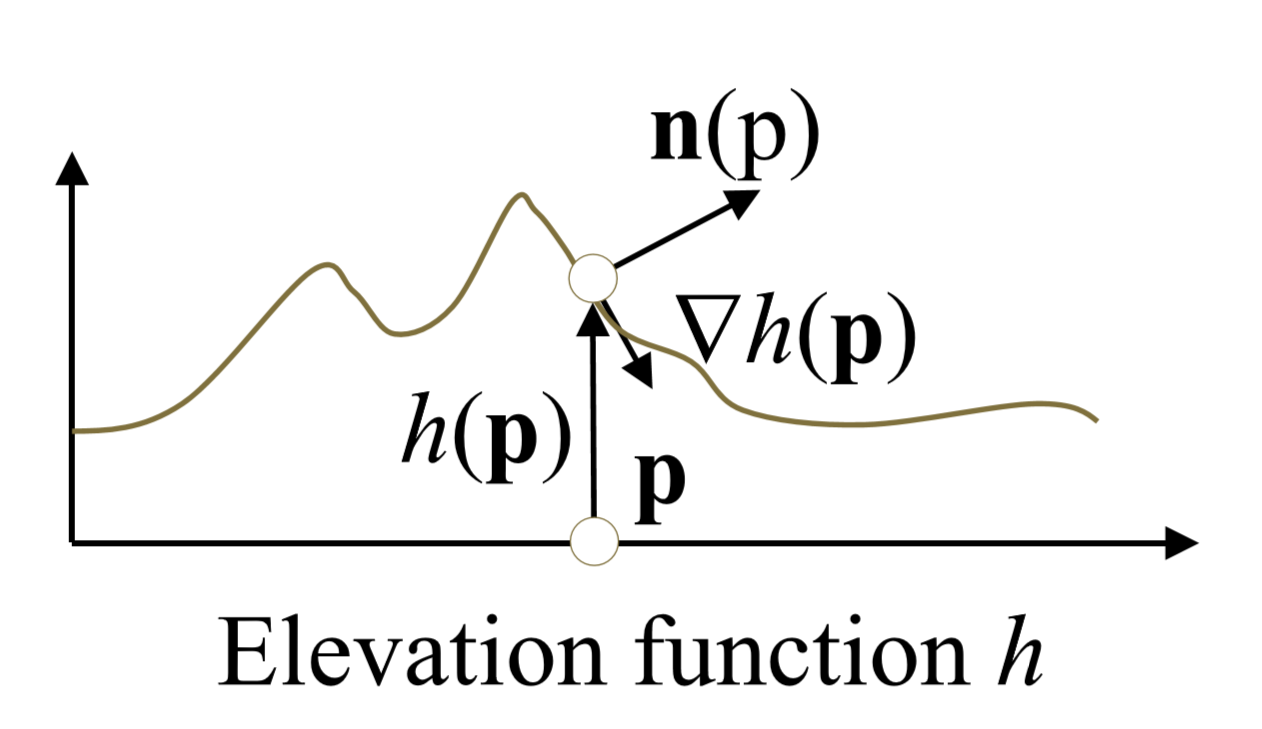
\includegraphics[height=4cm,width=6.9cm]{doc/example-utf8/figures/continue.PNG}
\caption{以函数形式表达高程\supercite{eric-review}}
\end{figure}
\paragraph{离散高度场表达}地形高程也可以由一组排列在规则2D网格上的离散高程值表达,并可以以灰度图的形式存储,称为高度图。这种表达方法不能模拟悬垂和洞穴等特征,但由于其能简单和有效利用存储空间,因此是工业界目前最常用的地形表达方式,被广泛应用于GIS应用、地形编辑工具、地形腐蚀模拟和游戏等领域。高度场数据通常由遥感卫星捕获得到,其精度受到网格大小和网格内部点个数的影响。要获得连续的表面数据需要在格点之间进行插值,通常的做法是对单元内的两个三角形进行两次线性插值。与函数表达不同,这种表达可以更好的支持不同形式的地形,但和过程式表达相比增加了内存开销。一种减小内存开销的方法是降低数据精度,用8位或16位表示一个数据。
\begin{figure}[htbp]
\centering
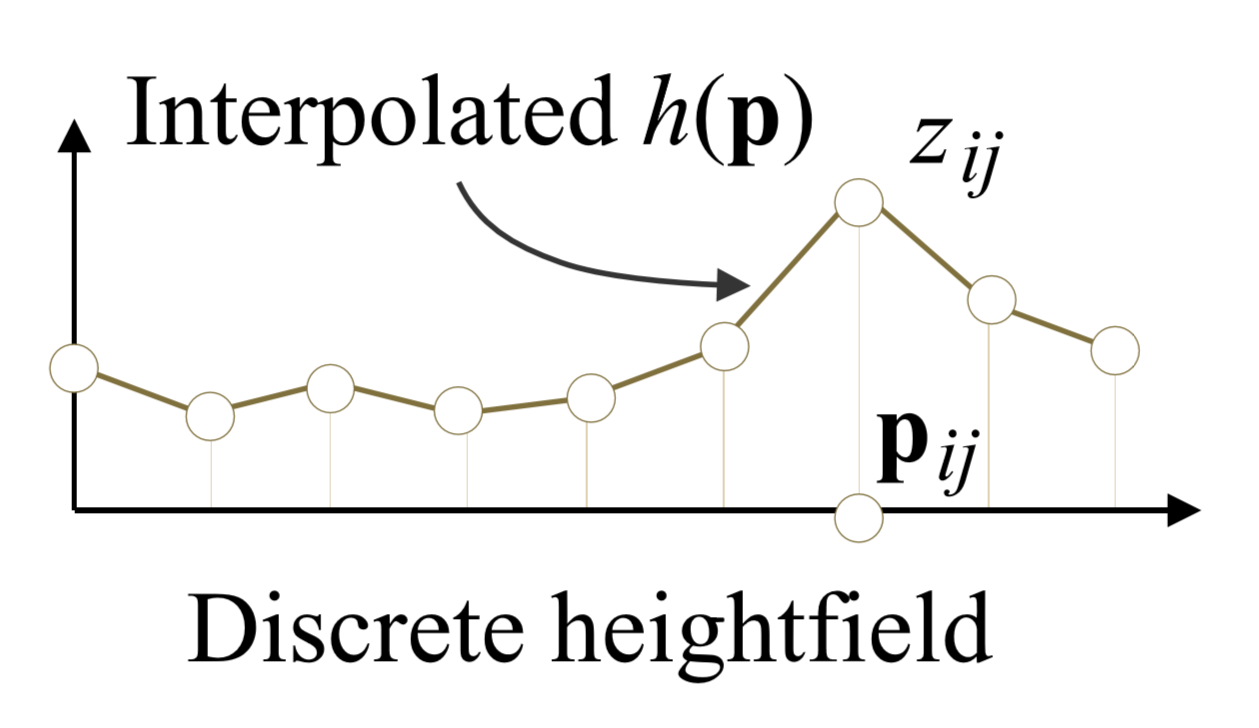
\includegraphics[height=4cm,width=6.8cm]{doc/example-utf8/figures/discrete.PNG}
\caption{以离散数据形式表达高程\supercite{eric-review}}
\end{figure}
大规模地形通常分块存储数据,以减少数据调度给内存带来的压力。网格数为$n$的块在每个网格格点上保存一个高程值,总共保存$(n+1)*(n+1)$个数据。为使地形块之间正确的拼接,对于索引为$(x,y)$的瓦块,其右边界与其右边块$(x+1,y)$的左边界相重叠,同理,其下边界与其下边块$(x,y-1)$的上边界重合。

\paragraph{体素表达}
体素表达可以捕获不同地质层的褶皱和断层,从而允许有悬崖、洞穴和拱桥的地形,解决了高度场表达不能反映地形的内部结构的问题。在这种方法中,空间被划分为3D规则网格,每个单元分配一个材质索引。由于进行了显式空间枚举,这种表达方法内存开销非常高,可以通过稀疏体素八叉树等技术进行压缩优化。此外,其离散特质使其不适合进行高精度的平滑地形建模,如非常平缓的斜坡等。\par
体素表达模型可以由一个函数定义$\mu:\mathbb{R}^3\to \digamma$,其中 $\digamma\subset\mathbb{N}$表示空间中任意体素所使用材质的索引。可以用单一材质的模型表示不具备语义信息的地形,即$\digamma=\left\{0,1\right\}$,其中0为空气,1为基岩。对于含有语义信息的地形,可以扩展索引集,使体素的材质索引表达语义信息,如图2.2。
\begin{figure}[htbp]
\centering
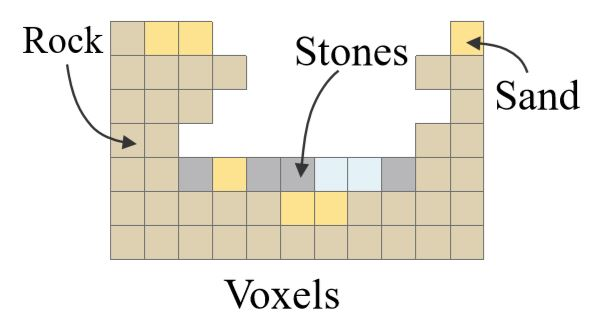
\includegraphics[height=3.8cm,width=7cm]{doc/example-utf8/figures/voxel.JPG}
\caption{体素表现允许拱桥、洞穴或悬崖的建模,但形状受其离散性的限制。\supercite{eric-review}}
\end{figure}

\paragraph{分层表达}
分层表达通过对地表不同沉积物的厚度进行建模来表达地形。Musgrave等\supercite{Musgrave1998The}提出了材质层的概念,并将不同材质层编码为一组有序的函数,这些函数在预先建立的层中描述厚度。其中底层表示基岩的高程,后续每一层表示其他物质的厚度,如岩石、沙砾、水等。这种数据结构是高度场表达法和体素表达法在空间效率上的折中,将体素表达法的数据压缩为了高度场的堆栈。此外分层表达法的垂直分辨率可以是无限的,而体素是离散数据,因此比起体素表达法,分层表达法可以更好的表达拱桥、悬崖等地形。以不同材质的复杂的动态堆栈管理为代价,分层表达法在地形腐蚀模拟中也得到了广泛的应用。
\begin{figure}[h]
\centering
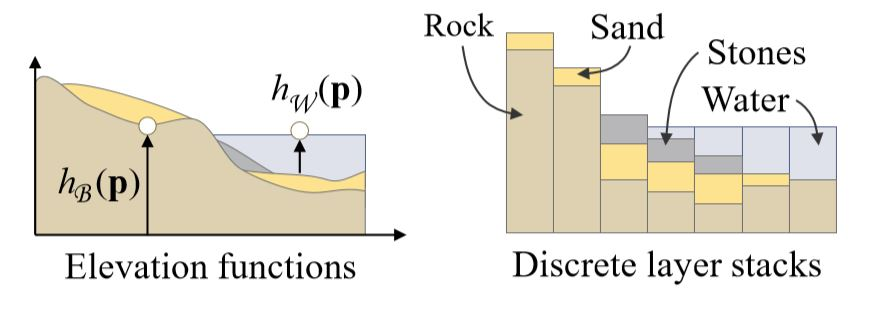
\includegraphics[height=4cm,width=11.5cm]{doc/example-utf8/figures/layer.JPG}
\caption{分层模型表达了按照预先设定的顺序组织的不同材质(从底向上依次是基岩、沙子、岩石和水)\supercite{eric-review}}
\end{figure}

\section{大规模地形实时渲染}
大规模地形数据的规模远远超过了标准图形硬件的能力,如果没有很好的地形表达和渲染算法的支持,就不可能以高细节层级交互式的进行可视化。在大规模地形实时绘制中,地形数据往往组织成四叉树形式。\supercite{Pajarola1998Large}
\subsection{地形四叉树}
地形四叉树是目前组织大规模地形的常用解决方案,它以分层的形式存储多分辨率地形数据,并将整个地形数据划分为若干个规则网格,每个网格被称为一个地形块。地形块在概念上被安排在不同的层次上,每个块上一层次的数据都被降采样到其一半的分辨率,类似于纹理数据的Mipmapping概念。如图2.5所示,每一层的网格被细分为许多大小相等的正方形块,每个块包含固定数量的高度值,块中的数据都是连续存储的。\par
\begin{figure}[H]
    \centering
    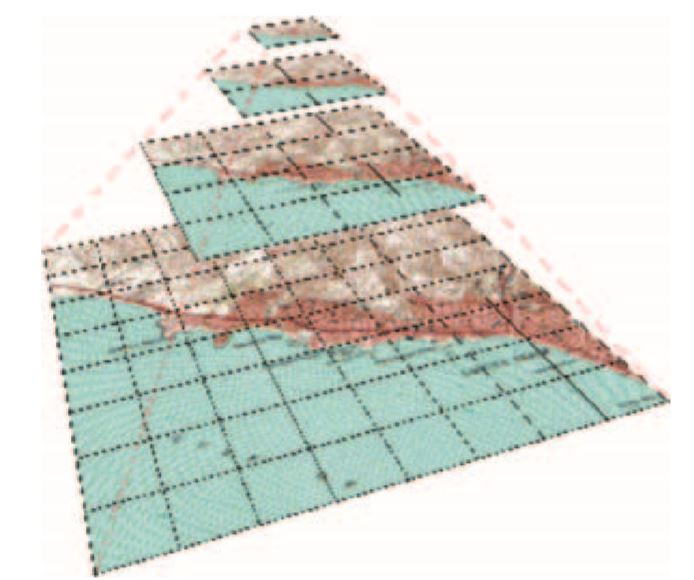
\includegraphics[height=4cm,width=4.8cm]{doc/example-utf8/figures/quadtree.jpg}
    \caption{存储为瓦块金字塔的地形\supercite{PlatingsCompression}}
\end{figure}
完整的四叉树存储意味着一个节点和它的子节点和邻居节点之间存在简单的位置关系,确定最顶层的经纬度范围和子块的大小后,各个级别之间的关系就被确定了,无需存储指针,可以直接从块索引中得到一个节点的位置关系。\par

地形四叉树根据视点位置来请求子节点,使CPU资源可以集中服务关键部分的数据。以不同层级渲染的地形块由于分辨率不同,可能会在地形块接缝处产生裂缝(图2.6),这种缝隙被称为T形连接(T-junction)。如图2.7所示,消除T形连接引起的裂缝有两种方法,第一种方法是将高分辨率网格中的边界点值与低分辨率点对齐。第二种是在低分辨率块中插入新点,并将值设置为高分辨率块中的对应点。第一种方法更加快速,但在网格边界高程变化剧烈的地形块上,减少三角形会降低画面质量,因此第二种方法视觉效果更好。
\begin{figure}[H]
    \centering
    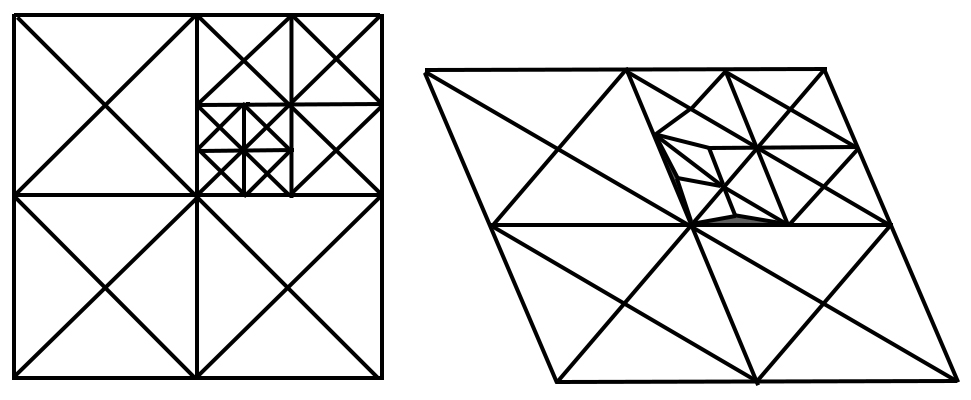
\includegraphics[height=3.5cm,width=9.2cm]{doc/example-utf8/figures/seam2.jpg}
    \caption{四叉树的三角剖分及产生的裂缝。左图中的黑点处可能产生裂缝,右图中的阴影部分显示了这些裂缝。\supercite{You2003Real}}
\end{figure}
\begin{figure}[H]
    \centering
    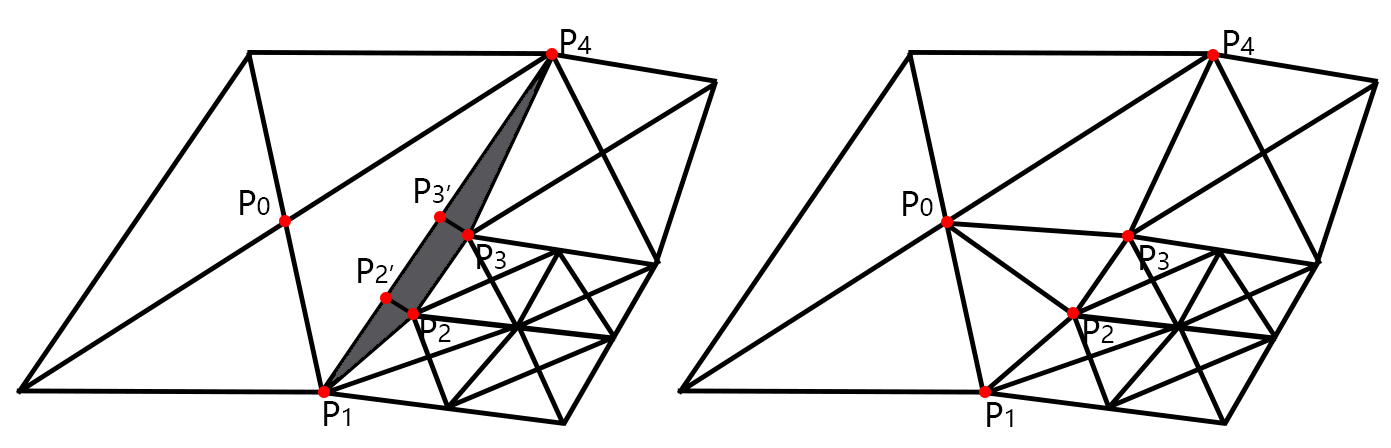
\includegraphics[height=3.7cm,width=10.2cm]{doc/example-utf8/figures/seamRepair.png}
    \caption{消除裂缝的两种方法。左图显示了第一种方法,将点$P_2$,$P_3$拉至点${P_2}^{'}$,${P_3}^{'}$处;右图显示了第二种方法,在低分辨率块中增加点,并与高分辨率块缝合\supercite{You2003Real}}
\end{figure}
\subsection{地形实时渲染技术}
大规模地形渲染的主要挑战是保证渲染效率的同时,兼顾地形的规模和精细程度。通过在CPU端对地形数据集的大小进行优化、在GPU端增添视觉增强策略等方法,可以提升地形的渲染效率和精细程度。下面介绍了实时渲染中一些实用的技术。
\paragraph{视锥剪裁}
为了最大限度地减少每帧渲染三角形的数量,需要对等待绘制的地形块进行视锥剪裁,将不在视锥中的块及其子块排除在外,使渲染性能显著提高。将地形块的包围盒与视锥体进行求交测试,与视锥相交的地形块被绘制,完全没有交集的地形块被直接抛弃,其数据不会被传输给GPU。在四叉树的数据结构中,如一个地形块的测试结果为不可见,则其子块也不可见。这个特性使剪裁算法可以非常快速的执行,减少了CPU的工作量。同时如果一个地形块完全位于视锥体内,则其子块也完全位于视锥体中,无需再进行测试。\par
视锥中的物体不一定都可见,也可能被其他物体遮挡而导致不可见。对于绘制地球的应用,地球自身遮挡其背面的地形,位于观察视角地平线下的地形块是无需绘制的,因此还可以进行遮挡剪裁来提升效率。

\paragraph{数据请求预测}
稳定的帧率对于仿真类应用有重要的意义。在对大规模地形场景进行渲染时,假设有三个连续的场景,渲染时以三个连续的视窗体现,分别是$w_1$、$w_2$和$w_3$。为了实现块数据缓冲,当发送$w_1$的块请求时,同时发送$w_2$和$w_3$的块请求。三个窗口的块请求的优先级不同,在$w_1$中的块请求应该被设置为优先,而$w_2$的块请求中,除去与$w_1$公有的部分,其他部分应该设置为次优先,在$w_3$的块请求中,除去其与$w_1$和$w_2$公共的部分,应该设置为低优先级,如图2.8所示。因此,当场景移动到$w_2$时,系统发送$w_2$窗口的块请求,数据预测线程将直接从地形渲染涉及的缓冲区中获取数据,而不需要从磁盘中读取数据。可以根据每秒画面刷新的次数和在场景中的移动速度决定预测请求的半径。使用类似的技术,在固定路线的场景漫游或飞行视景仿真中可以提高画面帧率的稳定性。\supercite{Chen2010Design}
\begin{figure}[htbp]
\centering
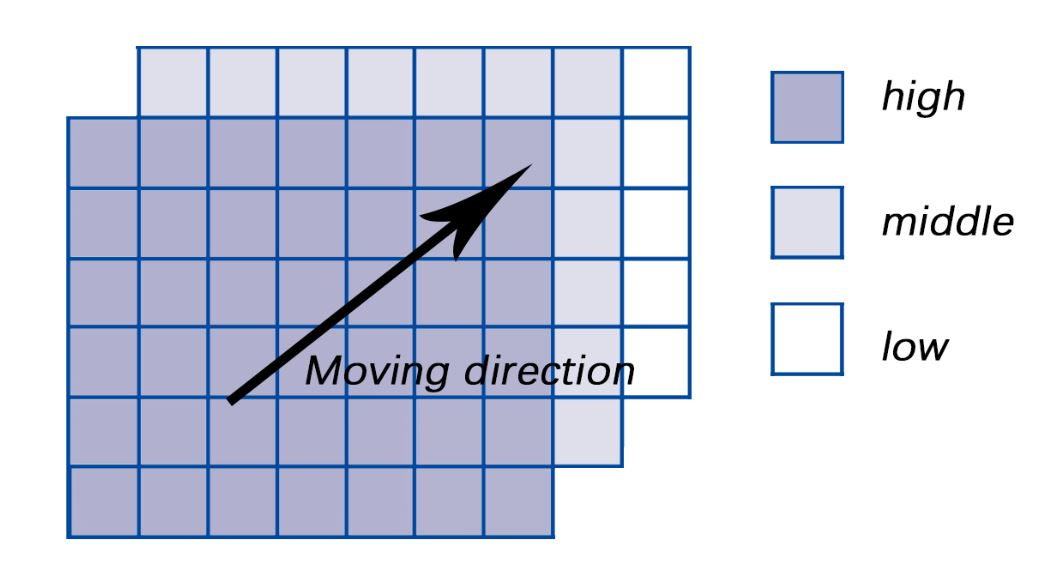
\includegraphics[height=4.3cm,width=7.8cm]{doc/example-utf8/figures/predic.JPG}
\caption{预测的数据块按高中低三个优先级进行顺序请求}
\end{figure}

\paragraph{过程式渲染}
过程式生成技术和硬件曲面细分技术允许在使用低分辨率的数据集情况下,仍然提供非常精细的地形可视化,而无需很高的存储开销。在游戏等许多应用中,地形数据高度值的准确性不是很重要,可以采用分形压缩算法将地形压缩成小而紧凑的数据集,并在运行时构建高精度的地形,从而大大减小地形数据的大小。为了动态的增强粗糙网格场景的细节,一个解决方案是在粗网格靠近相机的时候,通过程序过程式的细化粗网格或纹理。基于CPU的网格细化会被庞大的CPU-GPU几何数据流式传输所阻塞,为了避免这些数据传输,大量工作致力于通过利用曲面细分着色器直接在GPU上实现或模拟这些递归细分算法。Dachsbacher等\supercite{Dachsbacher2004Rendering}描述了一种动态向地形添加细节的方法,用数字高程图定义地形的大致形状,在渲染过程中,在图形硬件添加过程式的高程和纹理细节。Gu等\supercite{GuGeometry}将由草图生成的粗糙地形高度存储在几何图像中,并在绘制阶段加入详细的分形噪声。\par

\paragraph{贴花技术}
贴花是一种游戏开发中常用的贴图技术,其主要思想是在物体表面附加一张贴图,以实时的实现弹孔,血液喷溅痕迹,墙面涂鸦,脚印等等效果。此类技术有很多种表现形式,可以在物体表面附加半透明贴图、分层材质甚至模型。地形生成领域也可以将贴花技术用于为现有地表纹理添加高频率、高分辨率的细节,以极低的成本大大增加近地表漫游时的真实感。如在田野或机场的草地上添加草叶状图案、或在跑道和道路上添加砾石图案。贴花技术可以最小化顶点数,可以依据对渲染效果和效率的需求,轻松地调整低分辨率网格的LOD,且开销极低。因此,尽管在制作流程上需要一些额外的处理,但贴花技术有时可以作为地形曲面细分技术的替代方案。

\section{地形生成技术}
\paragraph{基于分形噪声的生成}
基于分形噪声的地形生成方法是一种过程式技术,此方法不模拟塑造地形的物理过程且不使用真实数据作为范例,而是通过对现实世界的观测直接重现现象。在观测中,真实地形常常表现出具有分形特征的分枝结构或树状图案,分形噪声可以很好的模拟出地形在多个尺度上的自相似性。分形噪声是早期的地形生成中最常用的过程模型之一,具有实现简单、效果良好、占用资源少等特性。\par
用分形噪声生成地形是在$\mathbb{R}^2$上定义一组经过缩放和变形的噪声函数\supercite{fbm},通过添加不同尺度和振幅的噪声,构建一个表示真实地形的函数。设$n$表示从$\mathbb{R}^2$到$[−1,1]$区间映射的平滑噪声函数,湍流函数$t$的定义是将不同频率和振幅的噪声贡献相加:
\begin{equation}
t(p)=\sum_{i=0}^{k-1}a_in(\Phi_ip)
\end{equation}
其中,$a_i$表示不同的振幅,$\Phi_i$表示不同频率,$k$表示噪声函数的个数。一般来说,振幅和频率被定义为一个几何级数:
\begin{equation}
\begin{aligned}
a_i=a_0p^i \\
\Phi_i=\Phi_0l^i
\end{aligned}
\end{equation}
其中$a_0$和$\Phi_0$是基础振幅和频率,$p$和$l$分别表示振幅的减益和频率的增益,在地形生成中通常将$p$设置为0.5可以得到有良好局部性和丰富细节的地形。噪声函数$n$的平滑性可以防止在山地地形中创建峰和脊线,如图2.9左图所示。因此为了产生诸如山峰或脊线之类的尖锐特征,可以引入脊线噪声。脊线噪声可以简单地定义为$r(p) = 1-|n(p)|$,其效果见图2.9右图。
\begin{figure}[htbp]
\centering
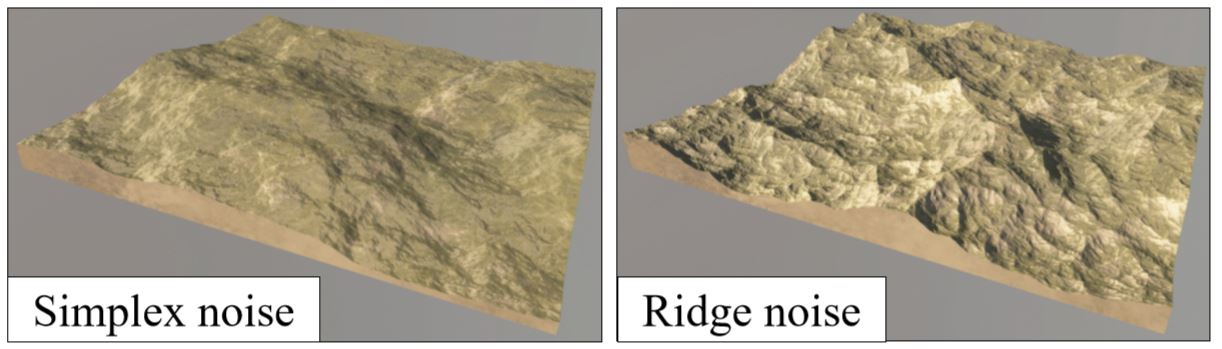
\includegraphics[height=3.5cm,width=11.4cm]{doc/example-utf8/figures/fractal.JPG}
\caption{分形噪声生成的过程式地形,左图为平滑噪声生成的地形,右图为八个不同频率的脊噪声叠加形成的多重分形地形\supercite{eric-review}}
\end{figure}
\paragraph{基于草图的生成}
基于草图的方法也称为基于特征的方法,该方法接受用户输入生成特征曲线,如山脊线,海岸线或河流等,并通过特征线将地形特征扩散至整个地形,从而生成匹配这些地形特征,且宏观上具有一致性的地形。Gain等\supercite{gain-sketching}的工作代表了最早的基于草图的方法之一,用于从控制曲线对地形进行交互建模。用户通过各种速写曲线来指定地形,可以输入的信息包括:基线(表示山脊在地面上的投影)、海拔(捕捉山脊的垂直形状)和边界(限制地形延伸到基线两边的距离)(图2.10)。\par
\begin{figure}[htbp]
\centering
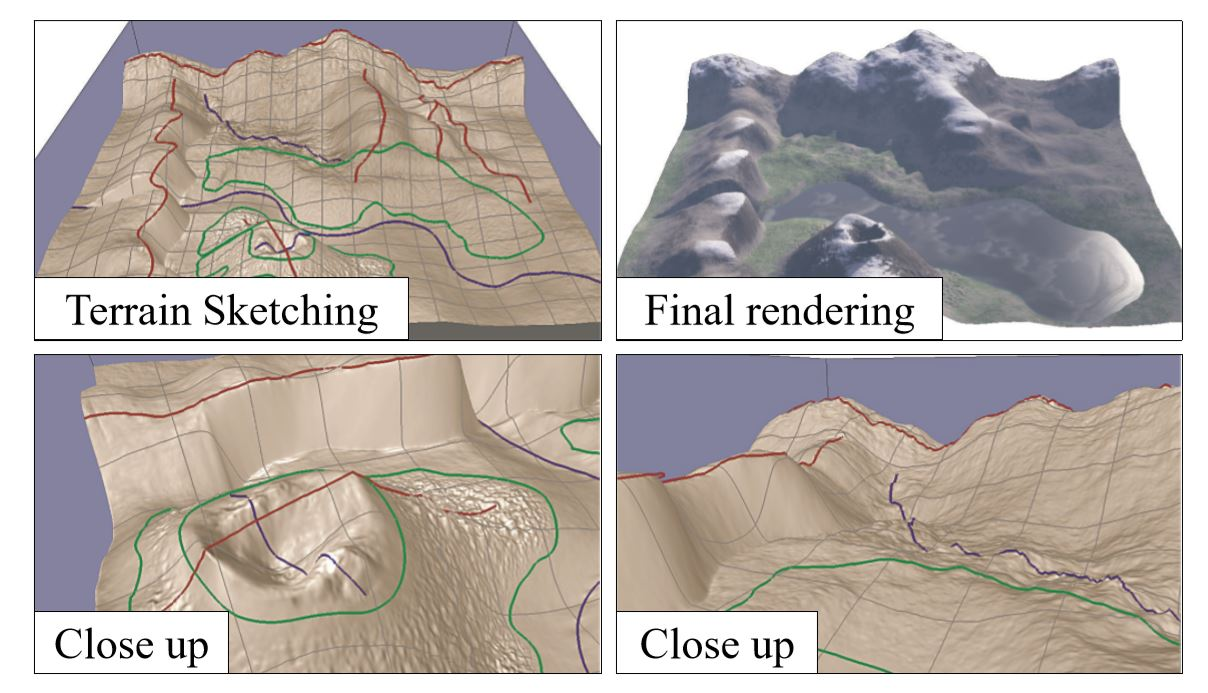
\includegraphics[height=5.6cm,width=9.9cm]{doc/example-utf8/figures/sketching.JPG}
\caption{草图可以将山峰、悬崖、火山锥、不同方向的小山和河流峡谷都在一个单一的地形中被描绘出来\supercite{gain-sketching}}
\end{figure}
Hnaidi等\supercite{HnaidiFeature}用特征曲线表示出山峰、河流和主要河流地貌的骨架,从而创建出地形。其使用带有附加信息的二维样条作为特征曲线,并描述了曲线每一侧的高程和坡度信息。由此产生的基于矢量的模型在内存中非常紧凑。噪声参数和梯度约束通过一个标准的扩散方程在离散网格中传播,对地形表面进行重构。通过使用扩散噪声参数合成的噪声图生成细节,向平滑的扩散地形添加细节来获得最终的地形。\par
基于特征的生成方法的提供了一种更直观的用户控制,但主要挑战来自于在整个地形上传播稀疏信息的困难,例如,在整个地形上传播山峰或河流等特定的地形信息。
\paragraph{基于仿真的生成}
过程式方法着重于一个特定现象的产生,而仿真技术注重模拟现象产生的原因和结果,因此能产生更真实的结果。地形仿真可以被看作是一个复杂的系统,在这个系统中,各种影响地形的元素相互作用产生了特殊的地貌。大部分的使用仿真技术的地形生成算法都是基于侵蚀的。侵蚀可以被抽象为一个三步过程,物质被侵蚀并从底层地形中分离出来,然后被介质运输,最终沉积在不同的位置(如图2.11)。侵蚀过程包括但不限于降雨和地表径流、河流和小溪侵蚀、海岸和海洋侵蚀、冰川侵蚀、风力侵蚀和大规模运动。\par
\begin{figure}[htbp]
\centering
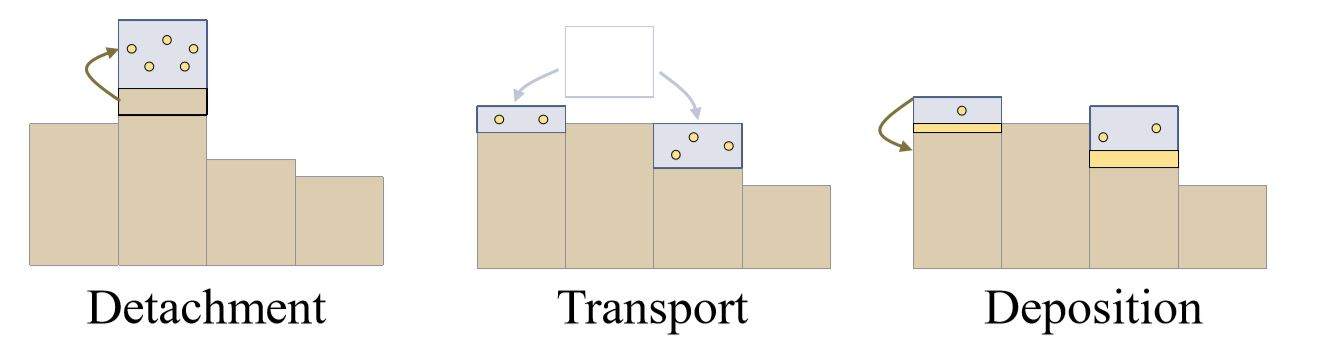
\includegraphics[height=3.6cm,width=12.5cm]{doc/example-utf8/figures/simulation.JPG}
\caption{侵蚀过程分离一些物质,由介质运输物质,最终沉积在不同的位置\supercite{eric-review}}
\end{figure}
Musgrave等\supercite{Musgrave1998T}在其工作中介绍了基于热力学的地形侵蚀方法。热侵蚀是热风化和物质运动相结合的产物,由于温度的变化,存在于物质缝隙中的水和物质本身产生了不同的热膨胀,引起物质的破裂,并在重力作用下向下运动。由此产生了宏观视角上,斜坡上的岩石和沉积物向下运动的现象。
\begin{figure}[htbp]
\centering
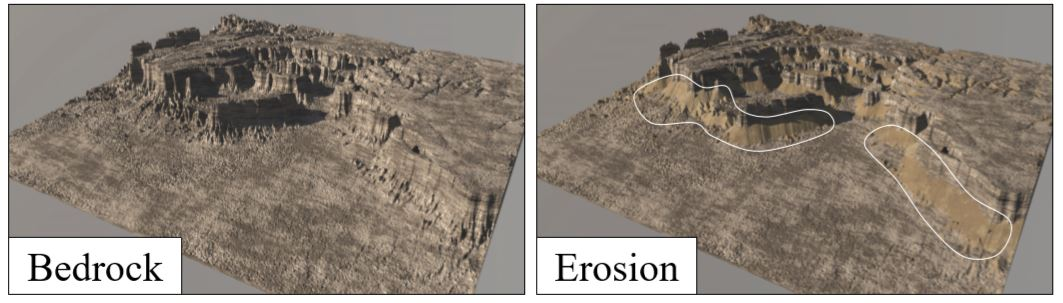
\includegraphics[height=3.5cm,width=11.4cm]{doc/example-utf8/figures/thermal.JPG}
\caption{热力侵蚀:左图是裸露的基岩,右图是热侵蚀形成的山岩和悬崖底部的岩屑和碎石\supercite{eric-review}}
\end{figure}
Benes等\supercite{Bene2002Visual}提出了一种水力侵蚀算法,算法通过一个离散的基于网格的模型来表示输入场景和流体,模拟水压力、水流速度和每个网格中的流体量。该水力模拟模型可以模拟水溶解土壤,转移土壤,并通过重力沉降将其沉积在不同的位置的过程。水力侵蚀可以在高峰之间形成深沟,而热力侵蚀可以正确地在岩石层创造岩石、沙子和颗粒物质,可以作为水力侵蚀的一个重要补充步骤。
\begin{figure}[htbp]
\centering
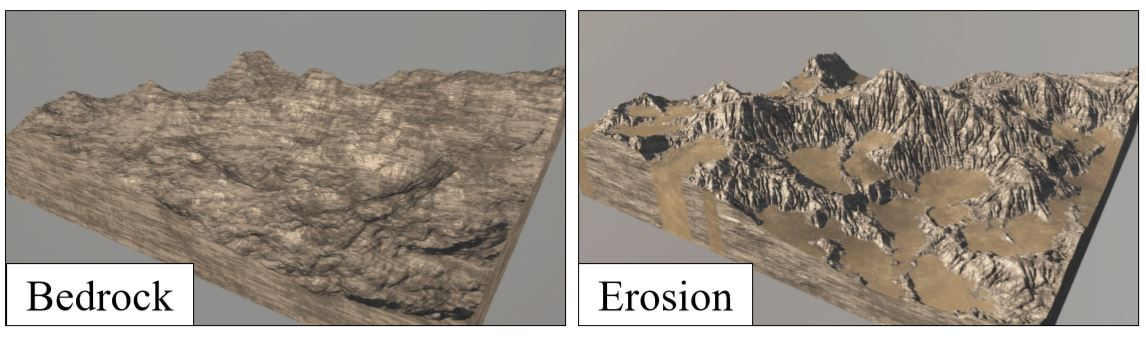
\includegraphics[height=3.5cm,width=11.4cm]{doc/example-utf8/figures/hydraulic.JPG}
\caption{水力侵蚀应用在过程式地形上的效果\supercite{eric-review}}
\end{figure}
\paragraph{基于样例的生成}
基于样例的方法借鉴并结合现有的地形,通过过程式方法或仿真方法逐步构建地形。样例地形的数据可以有多种来源,最常用的是来自于遥感卫星采样得到的真实数据,但也可以来自于过程式和仿真方法输出的地形。典型的基于样例的地形生成管线如下:(1)构建包含一个或多个地形样例的数据库;(2)执行分析步骤,从数据库中选择、扭曲和排列地形片段,并获取其高程函数;(3)将多个片段融合在一起,输出一个无缝的地形。基于样例的方法常常使用地形高程图作为算法的输入输出。Zhou等\supercite{Zhou2007Terrain}提出了一个基于纹理生成地形高度图的方法,该高度图受到用户输入的曲线特征的约束。给定一个用户绘制的草图和一个作为风格输入的真实地形,算法通过从真实地形复制像素块来创建一个新地形,这样用户草图中指定的曲线特征会呈现在输出中,且生成的真实地形具有与真实地形相同的小尺度特征。但是泊松接缝去除技术(一种去除重叠的块产生的人工痕迹的块合并技术)在3D光照下会产生明显的人工痕迹。此外用户只能指定山谷和山脊线的位置,2D草图不允许对这些特征线的高度轮廓进行直观的控制。Tasse\supercite{TasseEnhanced}等对这种技术进行了扩展,通过GPU并行计算降低了选取最佳块的成本,并减轻了多个块重叠造成的不自然痕迹。\par
\begin{figure}[htbp]
\centering
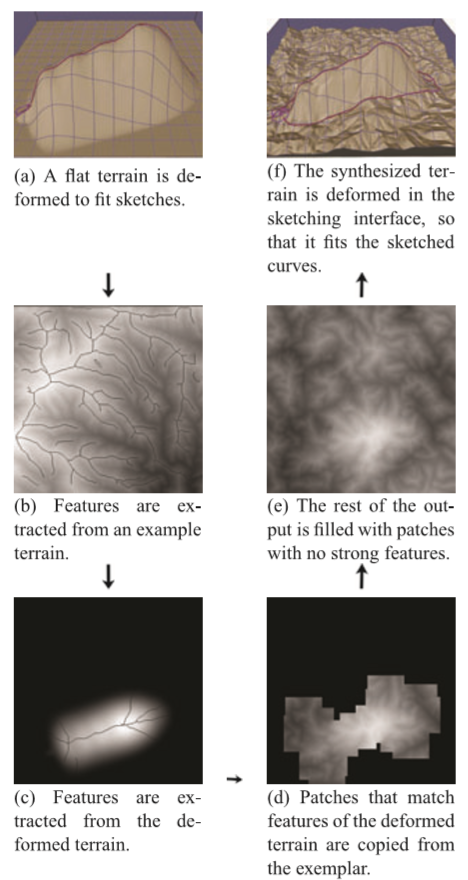
\includegraphics[height=11cm,width=6cm]{doc/example-utf8/figures/patchBased.PNG}
\caption{基于样例生成地形的工作框架\supercite{TasseEnhanced}}
\end{figure}
虽然这种方法快速、可控且生成的地形非常真实,但此类基于数据的方法需要上游训练阶段,且其结果高度依赖于输入数据的质量,采样的分辨率也局限于样例的分辨率,而公共可用的地形数据资源通常在每像素几米的范围内。

\section{地形生成结果评价标准}
对于给定的地形生成方法,有几个判断其有效性和实用性的标准。不同的应用场景依照其对各项标准的侧重,选择适合的地形生成算法。\supercite{eric-review}
\paragraph{多样性}
地球上有各种各样的地形,包括山丘、山脉、高原、峡谷和山谷等等。它们可能是由主要的自然事件或现象造成的,也可能是由许多不同因素在很长一段时间内的复杂相互作用造成的。地形可根据其高程、方向、坡度、土壤类型、基岩暴露状况等特征进行分类,地形生成算法能否产生多种多样的地形是评价标准之一。
\paragraph{真实感}
目前的地形生成方法中,在真实感方面普遍存在两个问题:(1)无法在不同尺度上都得到精确丰富的细节;(2)地形生成算法通常只能对一种现象进行模拟,难以将不同生成过程产生的地貌结合在一个地形中。评估地形真实感的一种方法是用地形渲染图对观察者进行用户调研,另一种方法是使用模拟水流对生成的地形进行排水的一致性测试。感性的和定量的评价方法不一定能得出一致的结论,因为某些现实世界的地貌,对从未见过此类地貌的观看者来说可能显得不真实。
\paragraph{用户控制}
为用户提供地形形状控制的机制和用户可以控制的程度也是考量地形编辑算法的重要标准之一。如何快速、直观地实现用户的意图,而不过分要求用户的地理知识储备,一直是地形生成领域的一个关键问题。在四十余年的研究历程中,科学家们已经提出了几十种基于过程、模拟和实例的地形生成解决方案。但由于在不同的尺度上所观察到的地形类型的多样性、地貌的复杂性和模式的多样性,不可避免地遗留了许多未解决的挑战。除此之外,已有地形编辑方法的可用性存在很大局限,例如虽然基于模拟的方法受到地质学和物理学的启发可以模拟真实世界中的地形现象,但其在直观控制和可用性上存在不足。这迫使设计师在一定程度上转向手动地形编辑,使用笔刷进行绘画、绘制矢量特征或对地形局部进行实时的形变,以实现他们的意图。笔刷提供了一种自然的方式来进行粗糙尺度的交互,然后可以通过过程式的方法生成更详细的地形。
\paragraph{规模} 
对地形生成方法进行评估时经常会忽略地形规模的问题,但范围和精度的对于地形生成问题是关键的,对于不同的应用程序有不同的要求,如在个人电脑上的游戏与飞行模拟器相比,地形面积更小但细节更多。假设规则网格边长为$a$,网格分辨率为$n$,则采样点之间的距离$a/n$为地形数据的精度。地形数据的计算成本随着$O(n^2)$的增加而增加,效率问题常常会限制分辨率,实时效率高的方法很难同时支持高精度和大范围编辑,有时会采取牺牲精度换取范围的策略。
\paragraph{效率}
时间和空间效率会影响地形生成算法在实践中的有效性,也可以影响到操作界面和用户体验。通常可以将地形生成算法的时间效率分为以下四个等级:实时级(每次更新耗时≤1/3秒)、交互级(每次更新耗时≤3秒)、秒级(每次更新耗时> 3秒但少于1分钟)和分钟级(耗时数分钟至数小时)。相对于完全预先设计好的地形来说,对于动态生成的地形,时间效率是至关重要的,而创作是相对次要的。\par
就空间效率来说,使用过程式方法和模拟方法产生的额外内存开销通常很低。然而基于实例的方法是数据驱动的,通常依赖于地形范例的数据库,因此有必要确定图形硬件的情况。

% vim:ts=4:sw=4

    \cleardoublepage
    % Copyright (c) 2014,2016,2018 Casper Ti. Vector
% Public domain.

\chapter{地形编辑器架构设计}
本文的地形编辑器基于ViWo系统的虚拟地球实现,虚拟地球的特点是地形数据量巨大,无法一次性载入内存,用四叉树分层组织数据,绘制时地形数据在内存中动态的换入换出。为了减少从硬盘读取数据的次数,系统中使用LRU算法对地形数据进行缓存,使地形数据可能有多个来源,这增加了数据同步的困难。为此,地形编辑器架构设计的首要目的是调度编辑所需的地形数据,将编辑结果正确的向多个来源、多个层级的地形数据进行同步,并实时显示在分层地形上。其次,地形编辑器可编辑的数据包括地形高程、纹理、语义等,这些数据虽然在数据格式、大小、内容和数据定义细节上有所不同,但形式上都是等宽高的二维数组。因此编辑器设计需考虑数据结构和编辑流程的可扩展性和复用性。本章介绍了系统中分层四叉树的数据管理和调度方式,并据此阐述了地形编辑器架构设计思路,最后对地形高程、纹理和语义编辑的通用流程进行了说明。\par
\section{基于分层四叉树的地形数据管理}                       
分层四叉树的每个子节点是一个地形块,其功能类似于“容器”,用于挂载绘制地形所需的多种数据,包括高程数据、纹理数据、蒙版数据和语义数据等。数据缓存块管理器用于代理地形数据的请求,四叉树向数据缓存块管理器请求地形块数据后,管理器将地形数据载入内存,并将数据以缓存块的形式驻留在缓存队列中。对于已经存在在缓存队列中的块,请求时按LRU算法调整缓存块在缓存队列中的位置以优化数据查找命中率,并将数据指针返回给地形块。地形绘制所需的多种数据的组织和调度方式基本相同,因此对数据缓存块类、数据缓存块管理器类等以模板的形式进行了实现,以便灵活的支持不同类型的地形数据。\par

本系统使用的地形数据块通过其在分层四叉树中的层数$level$、其横坐标$x$和纵坐标$y$进行索引和定位,$x$轴垂直于地球经线,沿经度递增方向递增,$y$轴垂直于地球纬线,沿纬度递增方向递增。每个地形块对应一个唯一的索引,系统中使用地形块进行管理的数据结构都以索引作为关键字进行存储。通过指定在分层四叉树中的层数,以经纬度为$(-180,-90)$的点作为原点,地球上某点的经纬度可以转换为其在数据库中的地形块索引。以经纬度为$(lon,lat)$的某点$k$为例,指定其层数为$level$,其所在地形块$b$的索引为$i_b=(x,y,level)$,有如下关系:
\begin{equation}
\left\{ \begin{aligned}
&originlon=-180\\
&originlat=-90\\
&x=floor((lon-originlon)/(180/(2^{level})))\\
&y=floor((lat-originlat)/(180/(2^{level})))
\end{aligned}\right.
\end{equation}

已知地形块$b$的索引,可快速获知其父子节点索引。$b$与其父节点$p$的索引$i_p$和其子节点$c_1$、$c_2$、$c_3$、$c_4$的索引$i_{c1}$、$i_{c2}$、$i_{c3}$、$i_{c4}$坐标存在如下关系:
\begin{equation}
i_p = (x/2,y/2,level-1)
\end{equation}
\begin{equation}
i_c = \left\{ \begin{aligned}
&(x*2,y*2,level+1)\\
&(x*2+1,y*2,level+1)\\
&(x*2,y*2+1,level+1)\\
&(x*2+1,y*2+1,level+1)
\end{aligned} \right.
\end{equation}
分层四叉树地形绘制的基本流程为(1)遍历四叉树,找到所有符合精度要求的覆盖地形的四叉树节点;(2)根据视口对节点进行剪裁;(3)获取待绘制节点的数据;(4)向GPU打包发送数据;(5)在GPU绘制。在虚拟地球的使用场景中用户视角是不断变化的,因此基于以上所示父子节点的关系,在视角运动的过程中,每一帧都重新自顶向下的构造分层四叉树。构造时遍历四叉树的子树,若节点精度不满足当前视角所需的分辨率,地形块会分裂为四个子块,即继续检查该节点的四个子节点。直到子节点的数据精度满足某个阈值,则停止分裂,并向数据缓存块管理器请求这些子节点的数据。\par
数据请求发生时,数据缓存块管理器首先从LRU缓存队列中查找地形块缓存,如果存在,则将缓存块的指针赋给地形块节点使用,如果不存在,则发起从本地获取地形块数据的请求。地形高程和纹理数据在本地以BerkeleyDb\supercite{Db}的数据库格式存储,数据缓存块管理器以地形块索引作为关键字向数据库请求地形块数据。由于涉及大量计算、查找和数据传输操作,同步的从本地数据库请求数据的时间效率不能满足实时漫游的流畅性需求。系统中实现了线程池和任务队列来管理地形块请求任务,将地形块数据请求作为一个任务添加到任务队列中异步的处理。使用多线程进行数据加载可以使界面交互不会被数据请求阻塞。自顶向下异步的请求地形块可以保证绘制的连续性,视口中的画面可能经历从粗糙到精细的加载过程,当这个过程非常短时对视觉效果影响较小。
\par

\section{基于规则网格的实时编辑}
对基于规则网格的地形进行笔刷编辑时,需要考虑笔迹的形成方式、在内存中的表示方式、笔刷的性质(如形状、直径、硬度等)以及笔迹对网格数据的编辑算法等问题。比起在单层地形上编辑,在分层四叉树上编辑的地形编辑器有诸多难点,包括编辑时笔迹所经过的地形块可能跨越多个层级、编辑结束后编辑结果向地形金字塔上层和下层的同步、首次从数据库中载入地形块后现有编辑结果向新载入块的同步,以及编辑结果在分层地形上的实时呈现等等。在分层地形编辑器中实现笔刷编辑需要对以上问题进行设计,兼顾鲁棒性和时空效率。\par
\subsection{编辑器架构}
地形模块是ViWo系统的核心模块,地形编辑器则以插件的形式,独立于地形模块存在。地形模块对地形数据的操作主要为获取地形数据、缓存地形数据、用地形高程和纹理数据进行绘制,同时其他模块还会通过地形模块提供的接口获取语义数据。地形编辑器在设计时需要将地形编辑逻辑与地形模块基本流程进行拆分,不启用地形编辑器插件时基础地形模块的绘制效率和运行流程不受影响。为此,在地形模块定义基类,实现地形绘制所需的基本功能,并在编辑器模块对基类进行派生,以多态的形式使地形模块支持编辑功能。如图3.1所示,红框表示基础地形模块所包含的主要功能,蓝框表示地形编辑器所包含的主要功能。加载地形编辑器插件时,用派生类对象替换基类对象,将地形编辑功能注入到基础地形流程中。\par

\begin{figure}[htbp]
\centering
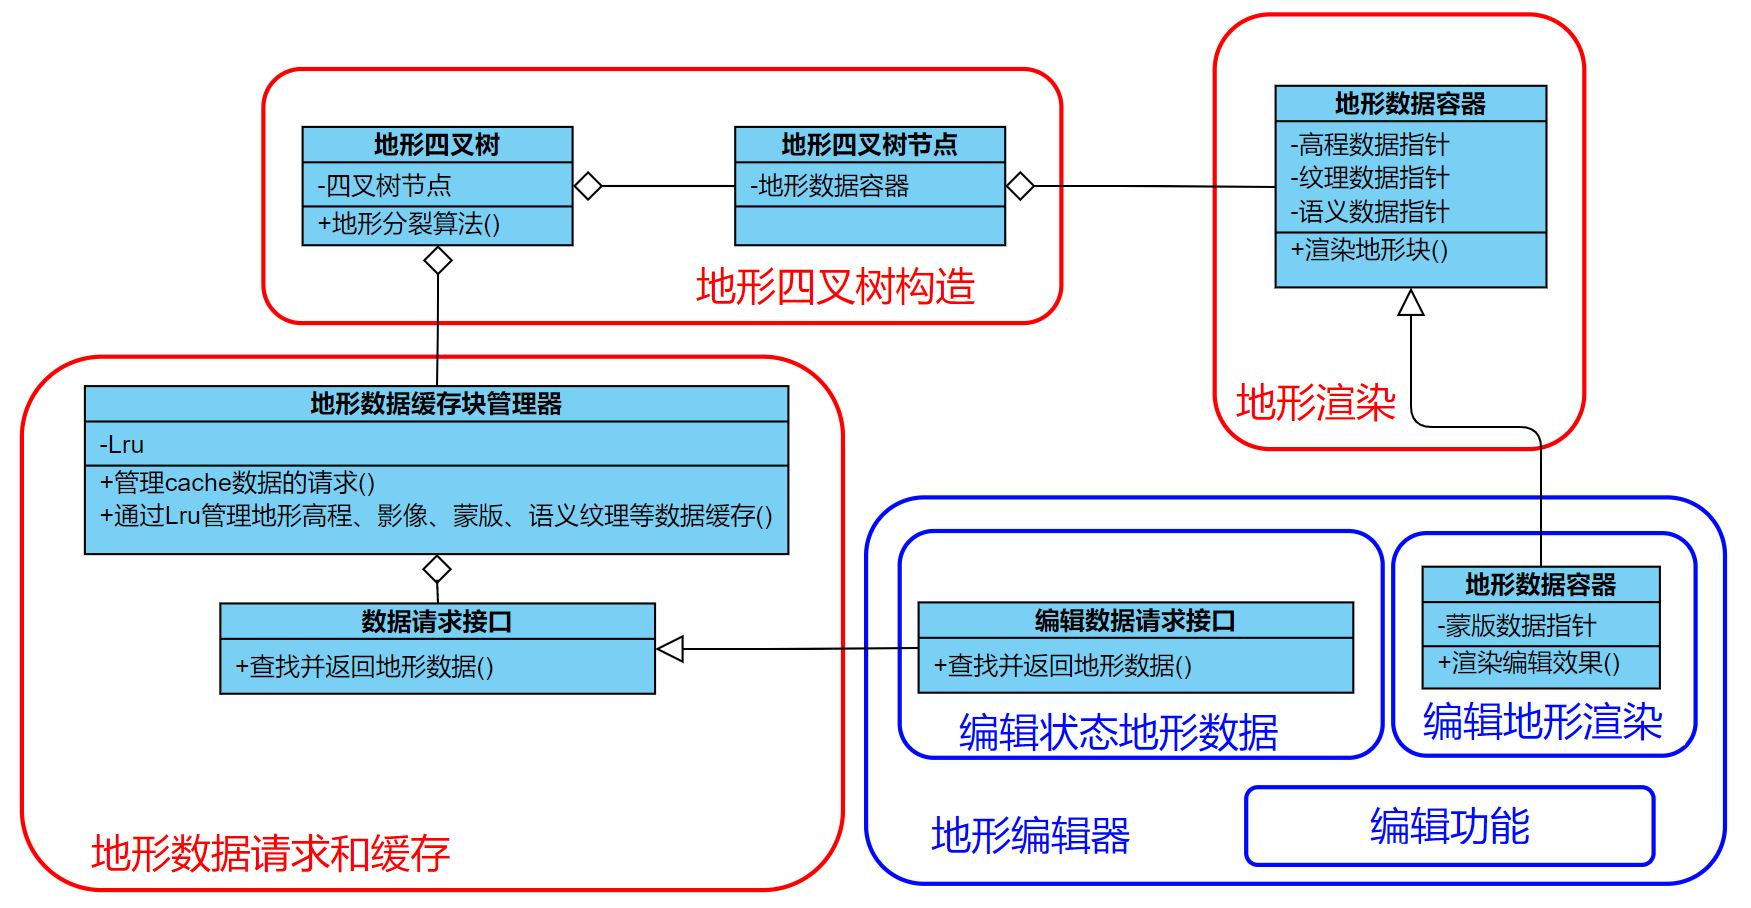
\includegraphics[height=7cm,width=13.2cm]{figures/editorStructure.JPG}
\caption{地形及编辑器功能模块图}
\end{figure}
本系统中用过滤\supercite{summer}来定义将编辑操作应用到高程数据上的过程,并定义过滤器为保存多次编辑操作的容器。编辑模式下请求地形数据时会经过过滤器,并检查当前地形数据上是否应用了所有编辑操作。考虑到使分层四叉树处于可编辑状态会带来额外的时间、空间开销,因此即便在配置文件中设置了加载编辑插件,也只在用户通过点击按钮开启高程和纹理编辑工具时,才替换基础地形数据结构为编辑状态的地形数据结构。由于分层四叉树每帧都重新构造,地形块内的数据也在四叉树构造时重新请求并挂载,因此在重新构造四叉树的过程中,可以自然的完成从普通状态地形块到编辑状态地形块的替换。实现中,在地形块内保存地形状态,在构造分层四叉树时通过检查当前地形状态是否与地形块内保存的地形状态相符。若不相符,则向地形块构造器重新申请地形块,并通过编辑模块派生的地形块构造器,构造具有编辑功能的地形块数据结构。对于数据缓存块管理器,不能用其派生类直接替换。因为LRU缓存队列包含了已经加载进内存的地形数据,重置数据缓存块管理器将导致现有的LRU缓存队列失效,并重新加载地形。因此不对数据块缓存管理器类进行派生,而是将其中数据请求相关的函数抽出作为一个类,对该类进行派生。
\subsection{编辑数据结构定义}
以油画绘制对地形的笔刷绘制做类比,可以认为一幅画是由若干笔迹构成的。产生笔迹的途径是使用画笔在画布上产生连续的若干个点,绘画者通过选择笔刷掌握笔迹的颜色、粗细、纹理、力度等特性。画布承载了画笔的若干条绘制结果,笔迹之间存在先后关系,从下到上按笔迹产生的顺序依次叠加在画布上。本系统中实现了笔刷、编辑曲线绘制工具、补丁数据等类,与笔头、画笔、局部画布等概念进行映射,下面对这些类一一进行阐述,并由图3.2阐述了类之间的关系。\par
\begin{figure}[htb]
\centering
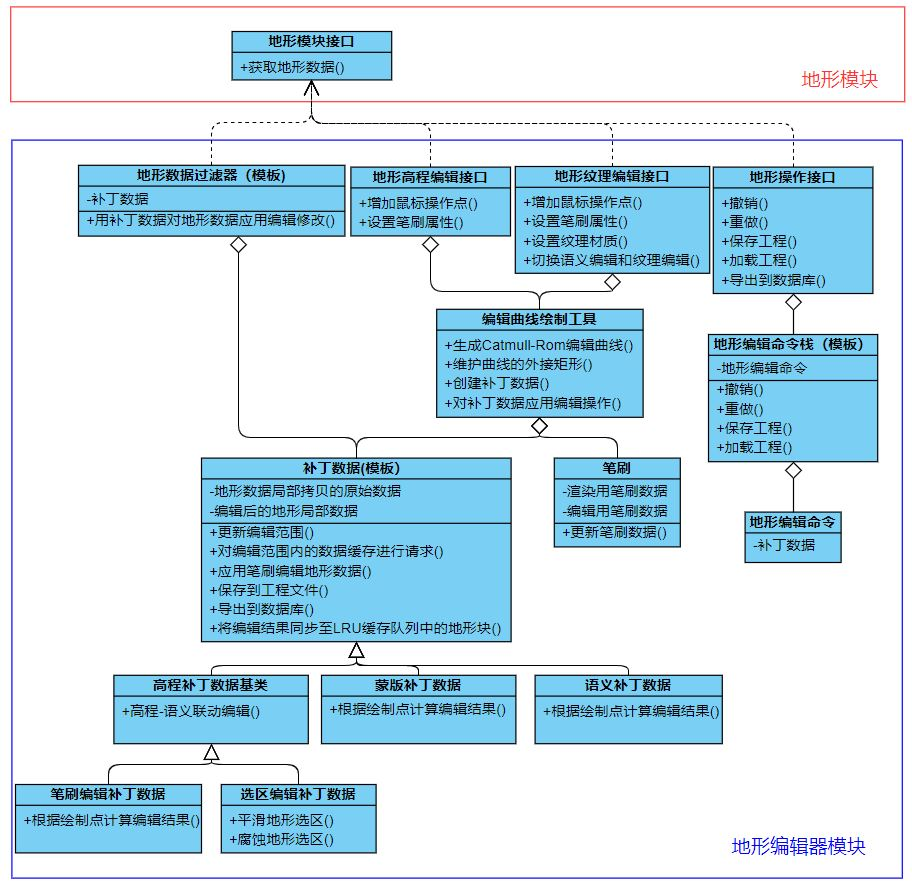
\includegraphics[height=12.8cm,width=12.5cm]{figures/structure2.JPG}
\caption{地形编辑器架构中核心类关系图}
\end{figure}
\paragraph{笔刷类}
高程编辑改变的是地形网格的高程数据,由测绘产生的地形高程数据本身分辨率不够高,网格不够密,因此更需要保持数据的连贯性,使编辑后的区域与未编辑区域可以平滑过渡。而地形纹理编辑的编辑结果需要有一定的随机性,看起来才更加自然。因此编辑器为高程和纹理编辑分别提供了两种笔刷,高程编辑为圆形笔刷,编辑强度从笔刷中心向笔刷边缘平滑降低。纹理编辑的笔刷以多种形状的笔刷模板的形式提供,编辑时笔刷模板中的每个数据与地表纹理中的数据一一对应,并指导在该像素处的颜色混合。
\paragraph{编辑曲线绘制工具类}
在本系统中,一次编辑操作定义为,一次鼠标按下拖拽并抬起的过程中,由若干离散鼠标采样点连成折线构成的单条笔迹。编辑曲线绘制工具的功能类似画笔,主要实现了将若干采样点转换为一条Catmull-Rom曲线,并控制具有大小、硬度等属性的笔刷在“画布”上进行修改的功能。Catmull-Rom样条曲线的一个特性是曲线经过所有控制点\supercite{catmull-rom},用离散采样点构造的Catmull-Rom曲线可以很好的拟合鼠标连续拖动形成的编辑笔迹。编辑曲线绘制工具从高程编辑接口接受鼠标轨迹采样点,构造Catmull-Rom曲线。鼠标点的采样频率与实时帧率相关,鼠标快速滑动或帧率发生波动时,两个采样点中间可能间距过大导致笔迹曲线不平滑。因此在两个采样点中间插入Catmull-Rom曲线上的点,插入的点称之为参考点。计算采样点之间的距离,使两个采样点间参考点的数目基本与距离成正比,使笔迹曲线样条形状更有一贯性,更加平滑。所有采样点和参考点统一作为绘制点参与笔迹绘制。目前笔刷的可调参数包括笔刷的直径和硬度,在此基础上,高程笔刷形状为圆形,纹理笔刷可以选择形状和编辑规则。在编辑曲线绘制工具的层面,对于高程和纹理编辑的笔刷编辑来说,增加笔迹点和生成笔迹曲线的逻辑是相同的,但在使用笔迹曲线对补丁数据进行修改的具体实现中,高程、纹理和语义编辑存在一定区别,分别在补丁数据的层面进行了实现,在本文后面的章节会进行详述。\par
\paragraph{补丁数据类}
编辑操作所保存的数据结构称为补丁数据,补丁数据是一块或多块相邻地形块高程或纹理数据的完整拷贝,可以看作“从画布上复制了画布的一块局部”。考虑一笔笔迹内所涉及的地形块在绘制时可能处于不同层,因此每开始一条笔迹时,即向编辑曲线生成工具添加笔迹的起始点时,生成一块新的画布。这块画布是现有地形的一个局部,包含之前所有的编辑结果。规定生成补丁数据时,拷贝原始数据的层级为当前分层四叉树中最精细层。笔迹的外接矩形表示了本次编辑的范围,此矩形与最精细层级的若干地形块相交,这些地形块的数据是直接参与本次编辑的,编辑前首先将其按原有空间位置关系拷贝到补丁数据中。编辑时对数据的修改首先应用到补丁数据上,并在编辑结束后,由补丁数据向LRU缓存队列中所有与补丁数据有交的块分发,即“将局部画布贴回画布上,覆盖画布中原有的内容”。如图3.3所示,某个局部区域中相邻的四个地形块上的编辑结果由三次操作产生的三个补丁数据按顺序叠加而成,可以看到第二个和第三个补丁数据上包含了之前的编辑结果。\par

\begin{figure}[htbp]
\centering
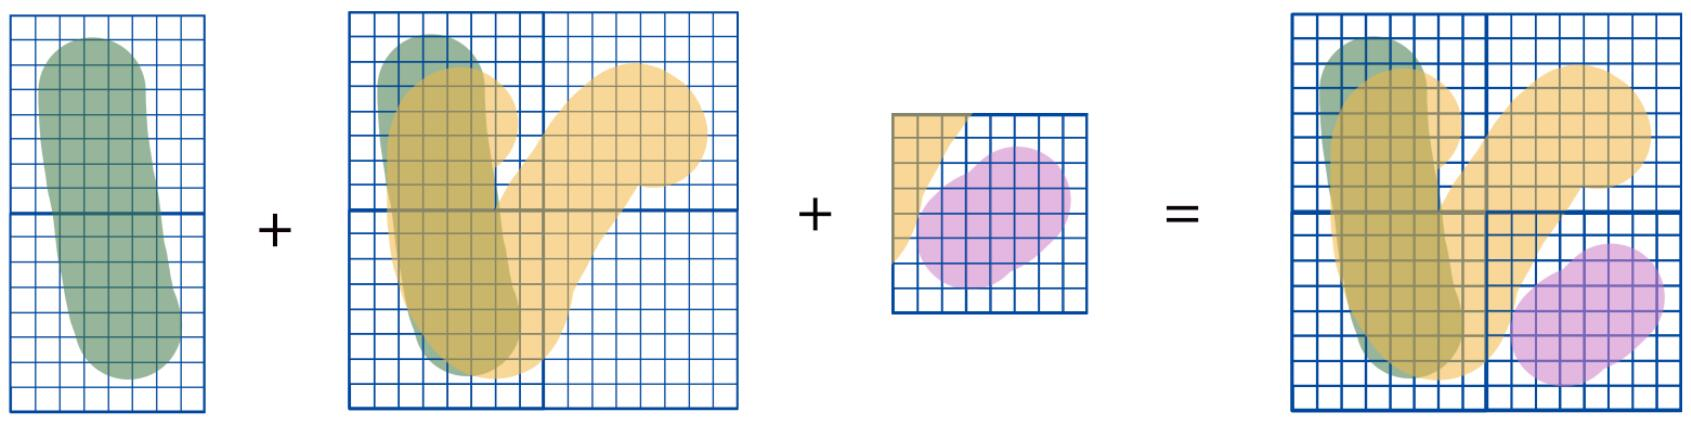
\includegraphics[height=3.9cm,width=14.8cm]{figures/mergeData.jpg}
\caption{补丁数据叠加作用形成最终的数据}
\end{figure}

\subsection{基于笔刷的实时编辑流程}
图3.4示意了笔刷实时编辑时编辑器的大致工作流程,流程的输入为若干个鼠标位置点,输出为一个编辑完的补丁数据,用补丁数据将修改结果分发到各个地形缓存块中后流程结束。\par
\begin{figure}[htbp]
\centering
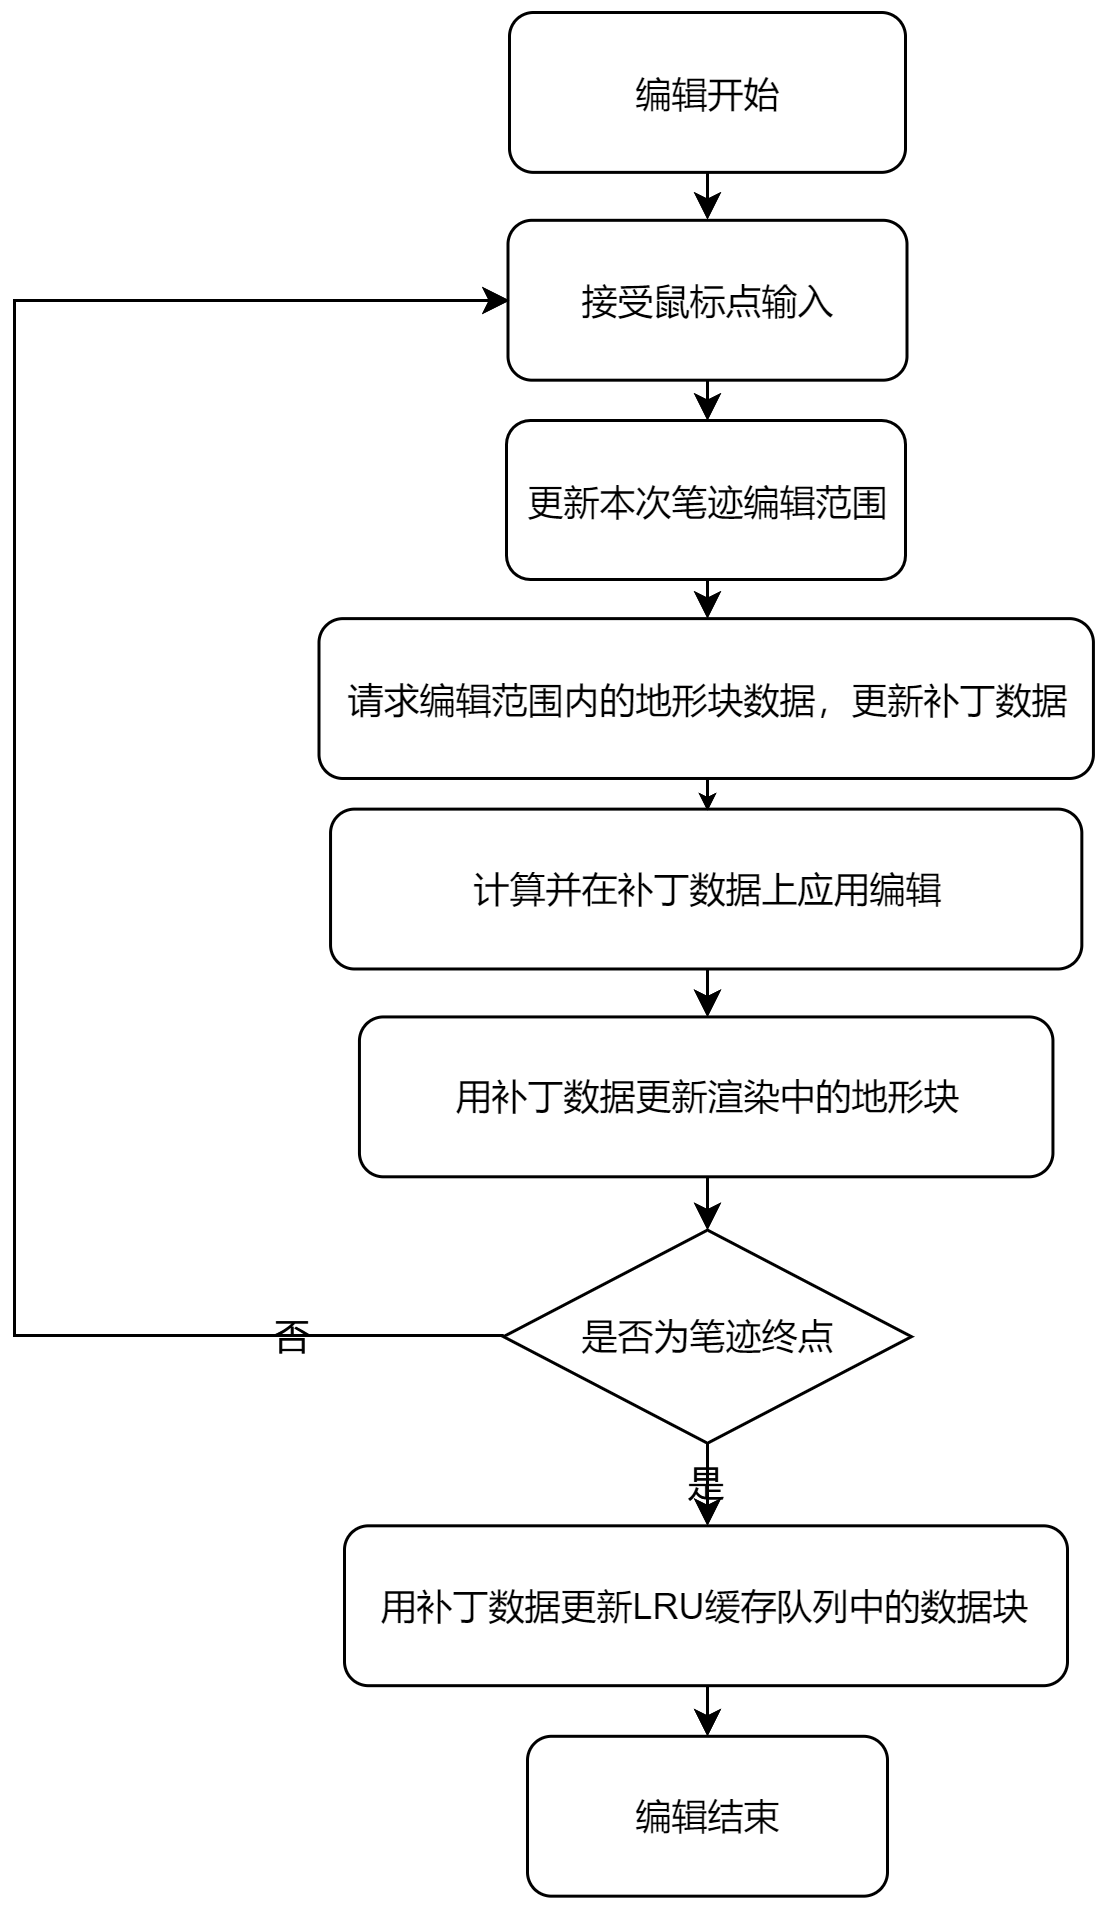
\includegraphics[height=11.6cm,width=6.5cm]{figures/flowChart.png}
\caption{笔刷实时编辑流程}
\end{figure}
一次编辑开始后,编辑曲线绘制工具根据当前分层四叉树的最精细层级创建一块初始的补丁数据,并清空上一次编辑的曲线数据,开始维护本次的编辑曲线数据。每向曲线中插入一个点,都会导致一次编辑范围的更新。图3.5展示了鼠标由位置\circled{1}拖向位置\circled{2},产生两个鼠标采样点的过程。平铺的蓝框表示若干地形块,其层级为当前分层四叉树中最精细的层级。红色和蓝色的同心圆分别表示笔刷的内直径和外直径,黄色和红色的虚线框和区域分别表示第一次和第二次更新编辑范围后,两个笔刷绘制点的外接矩形,及外接矩形与地形块求交得到的编辑范围。因此编辑范围发生变化时,为补丁数据重新分配内存,并对编辑范围内的地形块数据发起请求,拷贝原始数据填充补丁数据。\par
\begin{figure}[htbp]
\centering
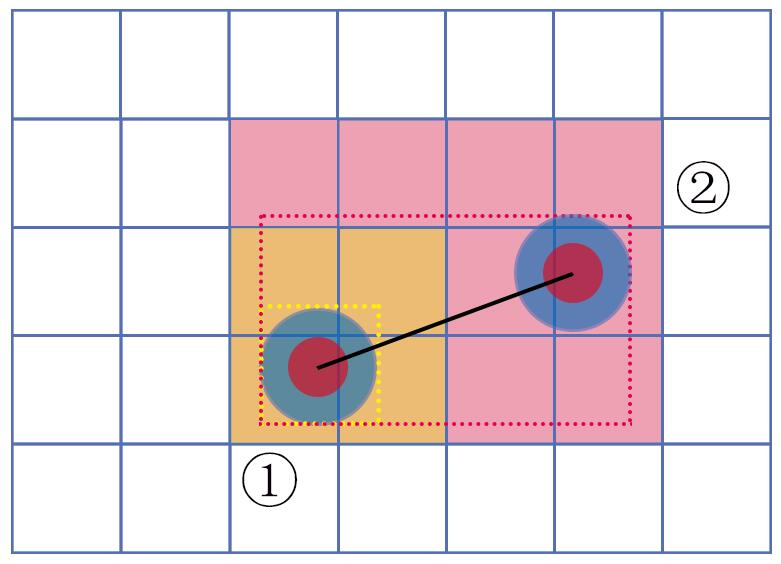
\includegraphics[height=4.3cm,width=6.2cm]{figures/brushRange.jpg}
\caption{编辑范围更新}
\end{figure}
称编辑时确定待编辑像素范围和数据变化情况的算法为笔刷编辑算法,高程编辑和纹理编辑分别对笔刷编辑算法进行了不同的实现,分别在第四、五章进行了阐述。\par
编辑结果从补丁数据向地形块数据的分发有两个阶段。第一个阶段是每接受一个鼠标采样点并对补丁数据进行修改后,将最新的编辑结果分发至补丁数据所覆盖的绘制中的地形块。这一阶段分发的目的是在用户拖动鼠标时实时的呈现编辑效果。第二个阶段是整条笔迹结束后,将保存了完整编辑结果的补丁数据,分发至地形金字塔所有层次中与该补丁数据有交且缓存在LRU队列中的地形块。这一阶段分发的目的是为了使编辑结果在地形金字塔的所有层次中同步。在第一阶段的分发中,由于补丁数据拷贝了最精细层级的数据,但处于绘制状态中的块并不都是最精细层级的块,可能是最精细层级的父块。因此对于补丁数据所覆盖的最精细层级块,如果当前绘制的并非该块而是其父块,则设置其父块为该块的关联块,并在第一阶段分发时分发到其关联块,以保证编辑结果的实时呈现。\par

补丁数据是保存了编辑结果的关键数据,应当能重复应用,使编辑结束后才请求到内存中的地形块也能正确的呈现编辑结果。因此,补丁数据创建后主动将自己注册到过滤器中保存。为了区分不同来源的数据块对编辑操作的应用情况,为数据块添加一个属性表示已经经过了多少次编辑操作。当对数据块进行过滤时,只对超出当前编辑次数的编辑操作进行应用即可。如本章上面内容所说,地形数据可能存在的位置有两种,一种是保存在本地数据库中的原始数据,另一种是绘制时被请求到内存中,并在LRU缓存队列中进行缓存的数据,发生数据请求时首先从LRU的缓存队列中查找块。过滤操作可以保证不同来源的地形数据都应用相同的编辑。对于LRU缓存队列中的地形块,编辑结束后立即应用编辑操作,使分层四叉树可以获得最新的地形数据。对于未在LRU缓存队列中的地形数据块,当分层四叉树从本地数据请求时,首先经过过滤器,将过滤器中的补丁数据依次应用到新请求的地形块上。\par

\section{编辑器常用功能实现}
对于编辑器来说,除了提供针对具体数据的编辑功能,还需要提供一些编辑器常规功能。在文件层面,对编辑结果进行文件存储和加载等操作,是使编辑成果可以保存和传输的必要功能。在操作层面,增加对编辑操作进行撤销和重做的功能可以提高编辑器的可用性和易用性。

\subsection{编辑操作撤销和重做}
本文基于设计模式中的命令模式,为高程编辑操作提供了撤销和重做功能。通过保存操作命令及其产生的核心数据,可以将操作命令队列保存至工程文件以保存编辑现场。命令模式是常用的行为型设计模式,其主要思想是将操作或命令视作一个对象来保存,并为命令类提供执行、撤销、重做等接口,从而灵活安排执行命令的对象和执行的时刻,降低系统的耦合度。通过正确的定义命令类的数据结构,保存执行命令所必需的信息,持有命令的对象可以复现该命令。\par
产生编辑结果的核心数据是笔刷的属性以及笔迹采样点,通过将这些数据传递给编辑曲线绘制工具,可以产生相同的编辑结果,但由于地形高程数据参与最终结果的插值,因此无法通过简单地将编辑高度设为相反数并应用原笔迹数据来撤销。编辑操作生成的补丁数据保存了当次操作前后局部地形的数据,因此编辑命令保存了补丁数据的指针。撤销时对补丁数据中指向原始数据和修改后数据的指针进行交换,并将原始补丁数据应用到当前地形上。即将补丁数据的编辑范围与LRU缓存队列中地形块进行求交,更新与之有交集的地形块数据。\par
使用双栈保存撤销和重做的操作命令以实现命令的管理和保存功能。一个栈存储命令,称为DoList,另一个栈存储回退了的命令,称为UndoList。命令对象包含一个编号属性,记录命令的发生次序。为保证编辑操作是单线性的,每次有新的操作进入DoList时,清空UndoList。图3.6以标号表示操作的次序,3.6(a)示意了执行操作、撤销和重做命令时,管理命令的双栈中数据发生的变化,图3.6(b)、3.6(c)共同展示了一个撤销操作的实例。如图3.6(b)所示,数字代表一个操作命令,由小到大表示编辑发生的次序,黑色数字表示现在应用的编辑,灰色数字表示回退了的编辑,为保证操作历史的单线性,当6号操作出现时,就需清空UndoList,栈内数据的变动如图3.6(c)所示。\begin{figure}[htbp]
    \centering
    \subcaptionbox{}{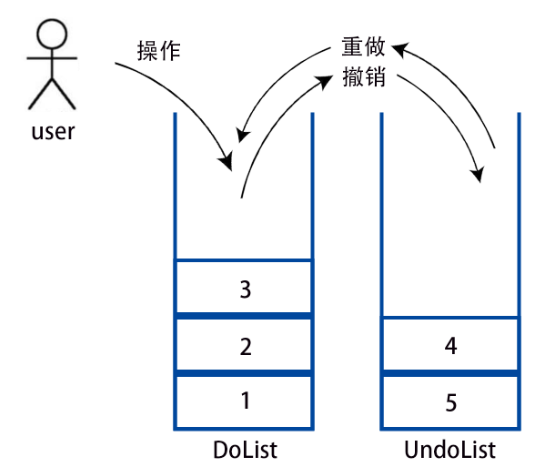
\includegraphics[height=5cm,width=5.8cm]{figures/command.png}}
    \subcaptionbox{}{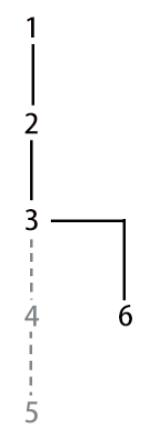
\includegraphics[height=5cm,width=1.5cm]{figures/command3.jpg}}
    \subcaptionbox{}{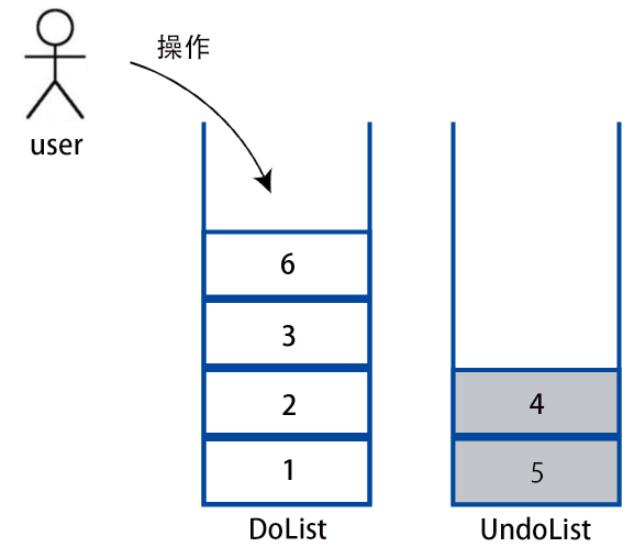
\includegraphics[height=5cm,width=5.8cm]{figures/command2.jpg}}

    \caption{以DoList和UndoList表示存储操作和存储回退的操作的两个栈:(a).操作、撤销和重做时命令对象在两个栈中的流动方向(b).撤销后未进行重做而进行了新的编辑的情况(c).如图(b)所示的情况需要清空UndoList以避免与编辑历史发生冲突}%The experimental results for $R_t= \exp \left( \left[1, -0.5, -2\right]^T \right)$.
\end{figure}
考虑到一个场景的编辑可能涉及上千条笔迹,因此为命令栈设置容量上限,只有容量上限范围内的命令可以撤销和重做,超出容量上限的命令数据可以进行合并优化。
\subsection{工程文件保存和结果导出}
编辑结束后,其结果需要以某种形式进行保存。目前要在系统中漫游精细地形需要配置的地形数据包括地形高程和纹理的两个数据库,为不使配置的复杂度增加,地形高程和纹理的编辑结果可以在导出时并入原数据库或输出到新数据库,用户可以通过配置数据库链式请求的顺序以应用编辑结果。同时,为了方便用户进行二次编辑,类似其他商用设计类软件的,应当提供一种工程文件保留编辑过程。因此分别实现了这两种保存方式。\par
对于写入数据库的保存,首先遍历过滤器,计算分层四叉树所有层级上需要保存的地形块索引,然后请求这些地形块,应用编辑操作后以原分辨率覆写到目标数据库中。以这种方法纹理编辑结果存储存在一定的弊端,一是保存前需要将纹理编辑所有图层的结果计算并叠加在一起,保存过程耗时较长;二是将纹理编辑结果的分辨率固定为与卫星影像源数据相同,分辨率下降,失去了纹理编辑产生的结果比卫星影像更精细的优点。\par
保存工程文件可以在一定程度上弥补写入数据库保存的不足。对于高程编辑操作的保存,命令队列中包含了开始编辑以来对地形高程执行的所有操作,因此对高程编辑操作的保存和加载就是对命令队列的存储和复原。实现中,分别保存Dolist和UndoList中的补丁数据,按顺序以二进制格式写入到本地文件中,需要保存的数据包括补丁数据的宽高、起止点等属性和地形数据本身。加载时,从文件中读取数据生成补丁数据,插入Dolist或UndoList,并注册到过滤器,用补丁数据进行过滤操作,使地形与之前编辑的结果相同。因此,当用户再次编辑时可以通过加载原始的数据库和工程文件恢复之前的编辑现场。对于纹理编辑操作的保存,需要按顺序保存每个图层的信息,包括图层名和图层所使用的纹理数据,以保证加载工程时可以还原图层的编辑状态,且无需在默认纹理库路径下配置之前使用的纹理材质。\par


\section{本章小结}
本章就分层地形编辑器架构设计中存在的一些难点进行了说明,并基于对这些问题的考虑,阐述了ViWo系统中地形编辑器的架构设计,介绍了该架构下实时大规模地形笔刷编辑,编辑操作的撤销和重做,地形编辑结果保存和加载等功能的实现方法。该架构还考虑了可扩展性,能应用在多种基于规则网格的数据的编辑上。下面两章将分别介绍高程和纹理编辑的实现细节和不同之处。
% vim:ts=4:sw=4

    \cleardoublepage
 	% Copyright (c) 2014,2016,2018 Casper Ti. Vector
% Public domain.

\chapter{基于多层地形的地形高程编辑}
对地形高程数据的常见编辑操作包括对地形高程进行抬高和降低、平整地形、平滑地形、腐蚀地形和对地形数据中的坏点进行修复等。笔刷是进行高程编辑最基本的工具,使用笔刷对地形高程进行抬高和降低,构造山峰、丘陵、山谷等地形,是地形高程编辑的常用手段。除笔刷编辑外,对地形进行选区编辑可以快速的对局部区域的整片地形进行平滑、平整、腐蚀等操作。地形平滑和平整功能可以为城市和机场等场景提供可信的地形环境,地形腐蚀操作可以模拟外部因素对地形的腐蚀作用,增强地形的真实感。\par
\section{基于笔刷的地形高程编辑}
高程编辑的笔刷为圆形,笔刷的大小存在不动性,即随视角高度的变化笔刷覆盖的屏幕像素数不变。编辑时,鼠标采样点以经纬度形式表示,因此将笔刷直径大小也换算为经纬度参与编辑范围的运算。一系列笔刷绘制点两两之间生成一个多边形,框定在地形数据中参与编辑的像素,若干个多边形连起来形成笔迹。设笔刷直径为$t$,首先将相邻的两个鼠标采样点$A$和$B$投影到地平面上,分别找到通过$A$点和$B$点的绘制曲线的垂线,在这条垂线上向正方向和负方向分别取得与$A$点和$B$点距离$t/2$的点作为多边形的四个顶点。如图4.1所示,图中红色点分别为两个相邻的绘制点$A$和$B$,绿色点为多边形顶点,根据绿色点$x$、$y$坐标的最大和最小值,在图中用蓝色点标出。蓝色的外框划定了计算时所需要遍历的像素的范围,这些像素与多边形进行求交,得到最终被编辑操作修改的像素,并由浅绿色标出。\par

\begin{figure}[ht]
    \centering
    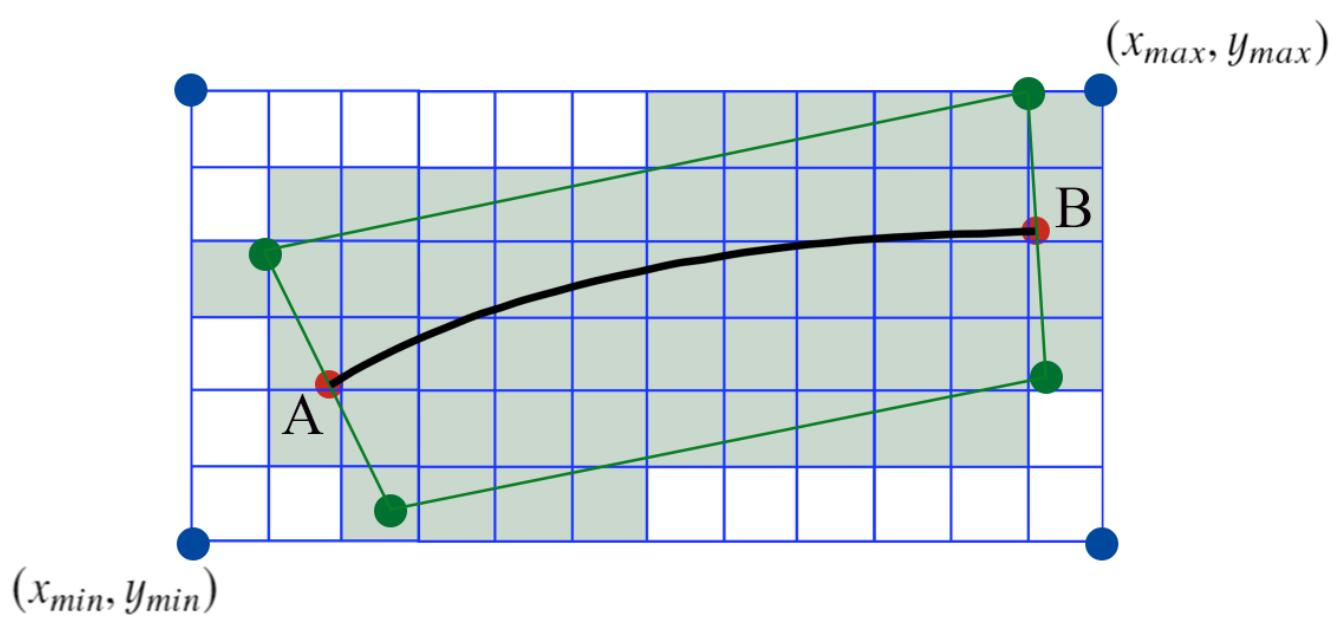
\includegraphics[height=4.7cm ,width=10.45cm]{figures/editArea.jpg}
  \caption{高程笔刷编辑范围}
  \end{figure}
设用户设定的笔刷的编辑高度为$H$,从笔刷中心向边缘,编辑高度逐渐降低,至笔刷边缘时降为0。对地形上某点$p$,其编辑高度$h(p)$由该点到距该点最近的绘制点的距离$d$和函数$f$决定:
\begin{equation}
h(p) = f \circ d(p)
\end{equation}
这里函数$f$选用了\textit{Wyvill field function}\supercite{wyvill},其定义域和值域都为[0,1],并随着输入值增大,从1平滑的向0过渡。该计算将笔刷覆盖范围内每个点与绘制点的距离映射为编辑后高度与原始高度混合的权重,可以实现从笔刷中心点向笔刷边缘编辑高度平滑减小的效果,该函数如图4.2所示。\par
\begin{figure}[ht]
\centering
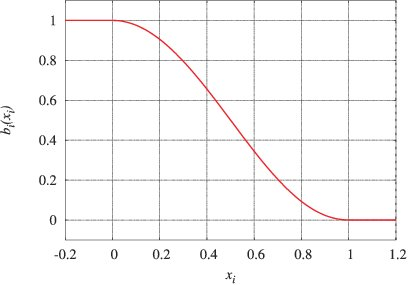
\includegraphics[height=4cm        ,width=5cm]{doc/example-utf8/figures/Wyvill-field-function.jpg}
\caption{Wyvill Field Function\supercite{wyvill}}
\end{figure}
对补丁数据中的某点进行修改时的计算如下:首先从其中获取原始地形高度$h_{start}$,并获取笔迹曲线上离该点距离最近的一个绘制点,取其高度$h_{line}$。由该计算的定义方式可知,编辑结束后绘制点的高度变为其原始高度与$H$的和,记为$h_{end}$。依据$h_{start}$、$h_{end}$和$d(p)$,编辑后高度$h_{result}$为:\par
\begin{equation}
\begin{aligned}
&  d_p=d(p)\\
& f(d_p) = 3 * d_p^2 - 2 * d_p^3\\
&h_{result}=h_{start} * (1 - f(d_p)) + h_{end} * f(d_p)
\end{aligned}
\end{equation}
使用地形平整模式进行笔刷编辑时,可以额外设定\textit{笔刷硬度}参数,该参数决定笔刷内直径与笔刷外直径的比例。笔刷内直径覆盖的面积内$f$的参数为0,即不参与与原始地形高度的混合,直接更新为用户所设置的高度值。笔刷内直径到笔刷外直径中间的部分按照$f$进行混合。\par
\begin{figure}[ht]
\centering
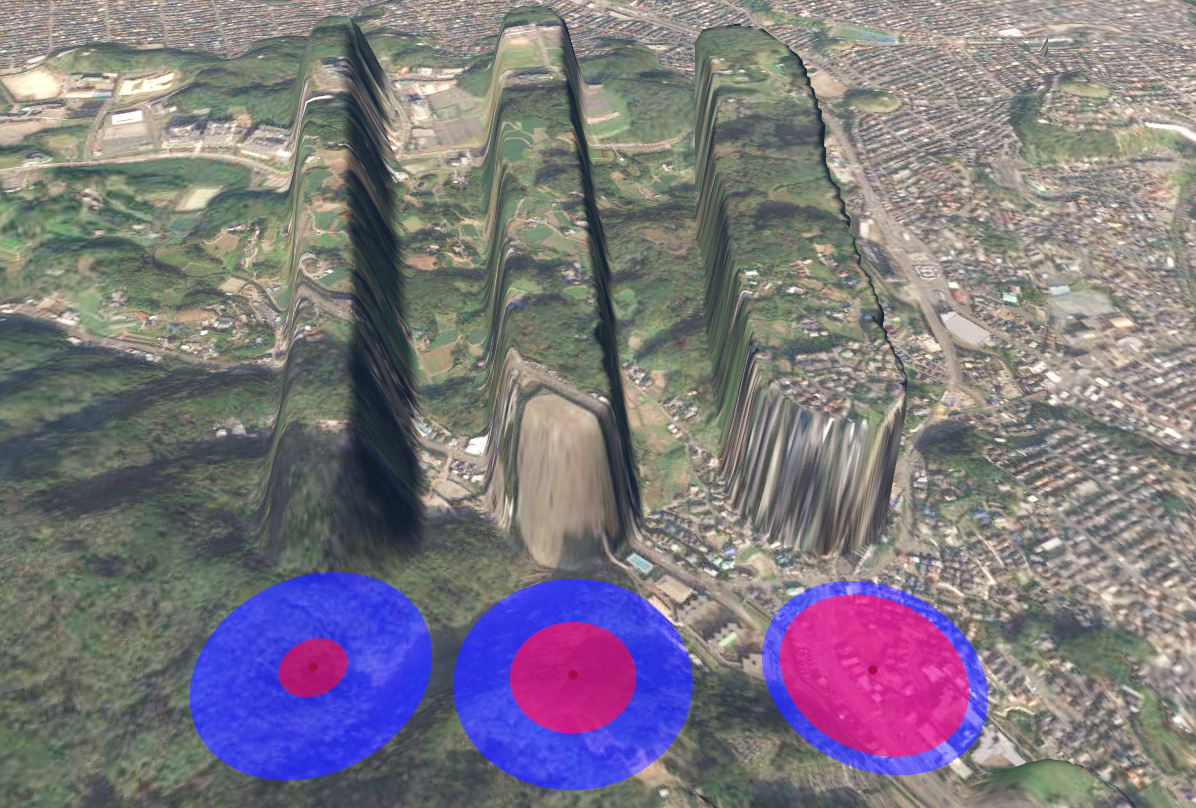
\includegraphics[height=4cm        ,width=5cm]{doc/example-utf8/figures/flatten2.jpg}
\caption{三种不同的笔刷内直径编辑的效果}
\end{figure}
为保证编辑操作的合理性,笔刷可设置的编辑高度区间在[-1000,1000]之间,笔刷最大直径为6千米左右,最高可在地形四叉树的第10层进行编辑。
\section{基于选区的地形高程编辑}
由于地形高程数据精度有限且存在误差,可能会在地表局部产生凹凸不平、尖刺和坑洞的现象。对于机场、城市等有近地漫游需求且需要地面平整来摆放模型的应用场景来说,需要提供一种编辑工具可以快速对地面进行平整。考虑到操作效率和简便程度,对地形块进行选区操作比笔刷涂抹更好。此外,还可以通过框选对地形进行腐蚀操作,腐蚀是模拟物理世界中水土流失的规律的技术,经过多次迭代后产生的效果可以很大的提升地型真实感。由于腐蚀操作需要进行数十次到数百次的迭代,因此在GPU端的实现更适应实时编辑的要求。地形平滑等功能需要对地形数据进行卷积滤波,也需要多次迭代以达到较好的效果。为了架构的清晰,地形平滑采用了和腐蚀一样的工作管线。\par
选区操作的实现特点是将地形高程数据采样为一张纹理图,在GPU中进行处理。这种方式打破了着色器只能更新当前所处理顶点的数据、无法访问同一网格中其他顶点的数据的限制,使腐蚀、平滑等需要获取某点邻域中的地形数据的算法得以实现。在得到补丁数据后,将补丁数据作为纹理传入GPU,由于地形高程数据的分辨率是2的幂,补丁数据的传输对图形硬件较为友好。经过片元着色器的运算后,将补丁数据渲染在一个UV值在$[0,1]$间的简单四边形面片上。将OpenGL视口的宽高设置为补丁数据的宽高,以使输入输出图片分辨率相等。用一个附加纹理的帧缓存作为接收结果数据的对象,在多次迭代中使用两个纹理交替做为输入和输出。\par
选区范围由鼠标在地形上点选拖拽生成,起点为鼠标按下左键开始拖拽的点,终点为拖拽结束松开鼠标的点。以地形四叉树最精细层级对地形块进行选择,与选区有交集的所有地形块都会被选中,一个地形块或者完全被选中,或者完全不被选中。为显示用户选择的选区范围,在鼠标拖拽时要实时渲染当前所选择到的选区边界。鼠标拖拽时鼠标当前所在经纬度被实时更新,选区边界以选区左下角和右上角的经纬度确定。由于经纬度向地形块索引的转换是向下取整的,地形块坐标系统的$x$和$y$值分别向右向上递增,原点在地图的左下角,因此对于地形块内的所有点,根据其经纬度计算索引,该索引转换为经纬度所在的点在该地形块的左下角,左下角的经纬度得以确认。对选区右上角的地形块索引的$x$、$y$值加1进行矫正,即索引为$(x,y,level)$的地形块的右上角即为索引为$(x+1,y+1,level)$的地形块的左下角。然后根据地形块索引和地形块所在层级每个块的经纬度尺寸,获取地形块左下角的数据,分别绘制选区的四条边。由于四叉树分裂算法的性质,多数时间视野中的地形块数量较少,但出于图形硬件的限制和对操作效率的考虑,还是对地形选区可框选的块数和选区所在层数进行了限制。\par
高程数据可以以高度图的形式表示,地形平滑可以看作对高度图进行平滑滤波,使高度图变得模糊,并消除图中的噪点。反映在地形上则减少了地形上某点与其邻域的高程差,消除了与邻域高程差过大的点。平滑滤波通常取相邻像素点的值,按固定权重进行平均,随着邻域的扩大,平滑效果会得到增强,但也存在边际递减效应。考虑到进行图片采样的时间消耗,系统中取目标像素八邻域内的像素,简单进行平均,可以取得较好的效果。由于只对高程数据进行改变,地表纹理数据中因高程起伏产生的阴影无法消除,视觉效果上依然存在不平整的感觉。但考虑到此功能的应用场景多为城市、机场跑道等建筑区域,且主要目的是为了更好的摆放模型、去除高程数据中的噪点,上述的缺陷是可以接受的。


\section{结果分析}
本系统中的高程编辑器界面设计如图4.4所示,使用时通过最上面的功能按钮切换当前使用的功能,并通过滑动条对当前功能提供的可调参数进行调整。通过点击下方的按钮可以进行操作撤销和重做,编辑结束后可以对编辑工程进行保存,也可以将编辑结果导出至数据库。图4.5展示了VIWO系统中旧地形编辑器的编辑界面。旧地形编辑器需要在进入编辑状态时固定编辑层级和编辑范围,本编辑器可以在浏览和编辑状态间无缝切换,可以更方便的从不同视角、不同层级进行编辑。
\begin{figure}[htbp]
    \centering
    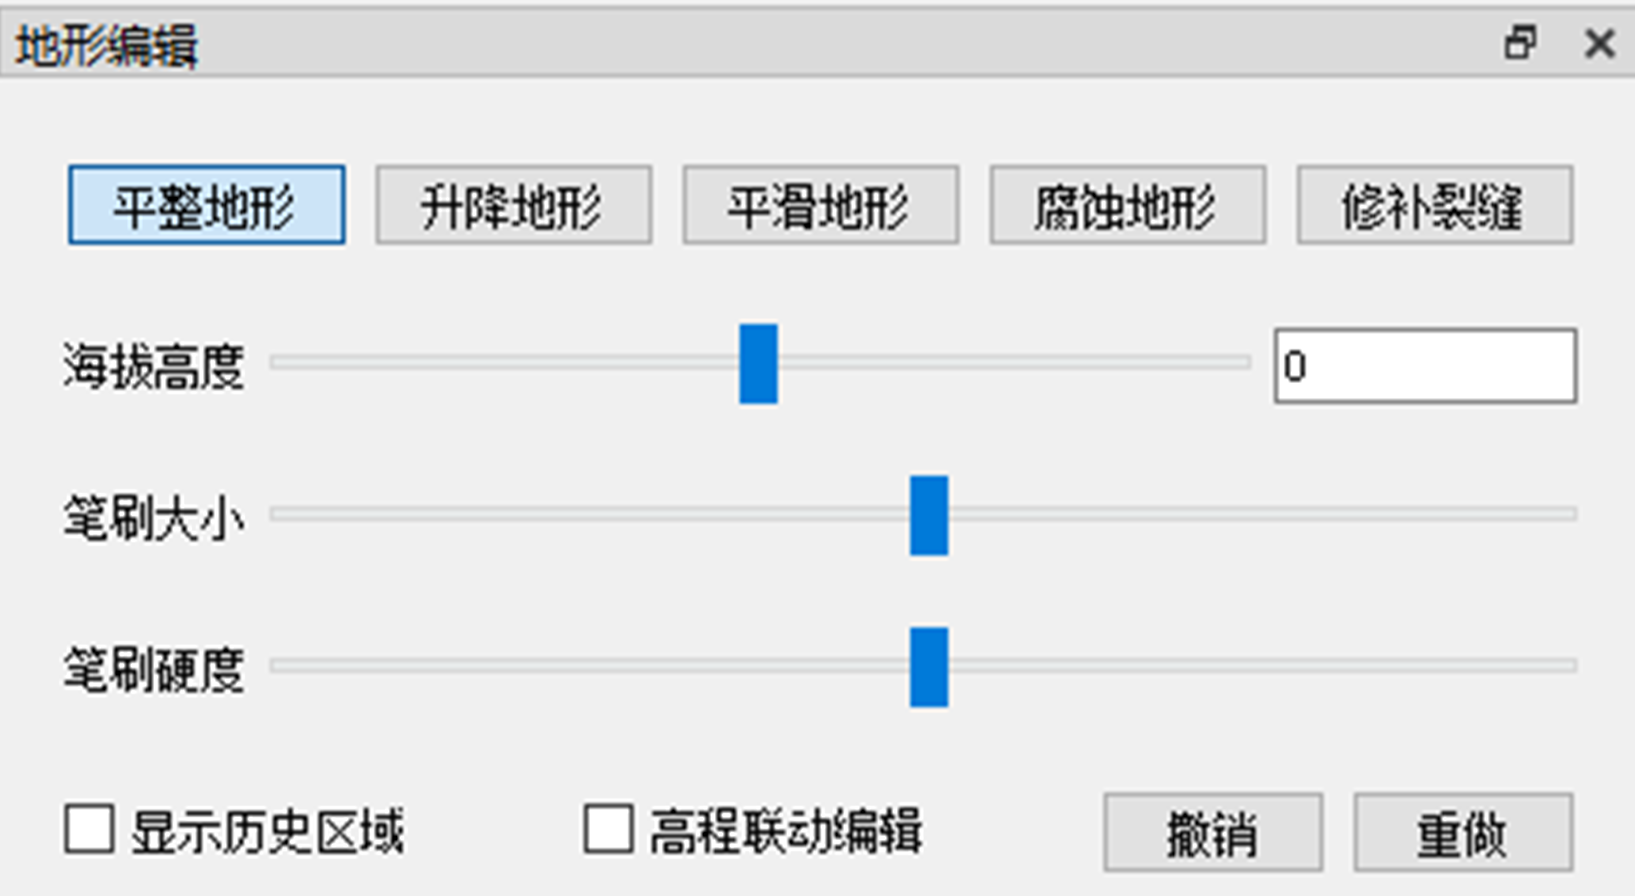
\includegraphics[height=4.9cm,width=8.6cm]{figures/demInterface.png}
  \caption{高程编辑器界面}
  \end{figure}
  
  \begin{figure}[h]
\centering
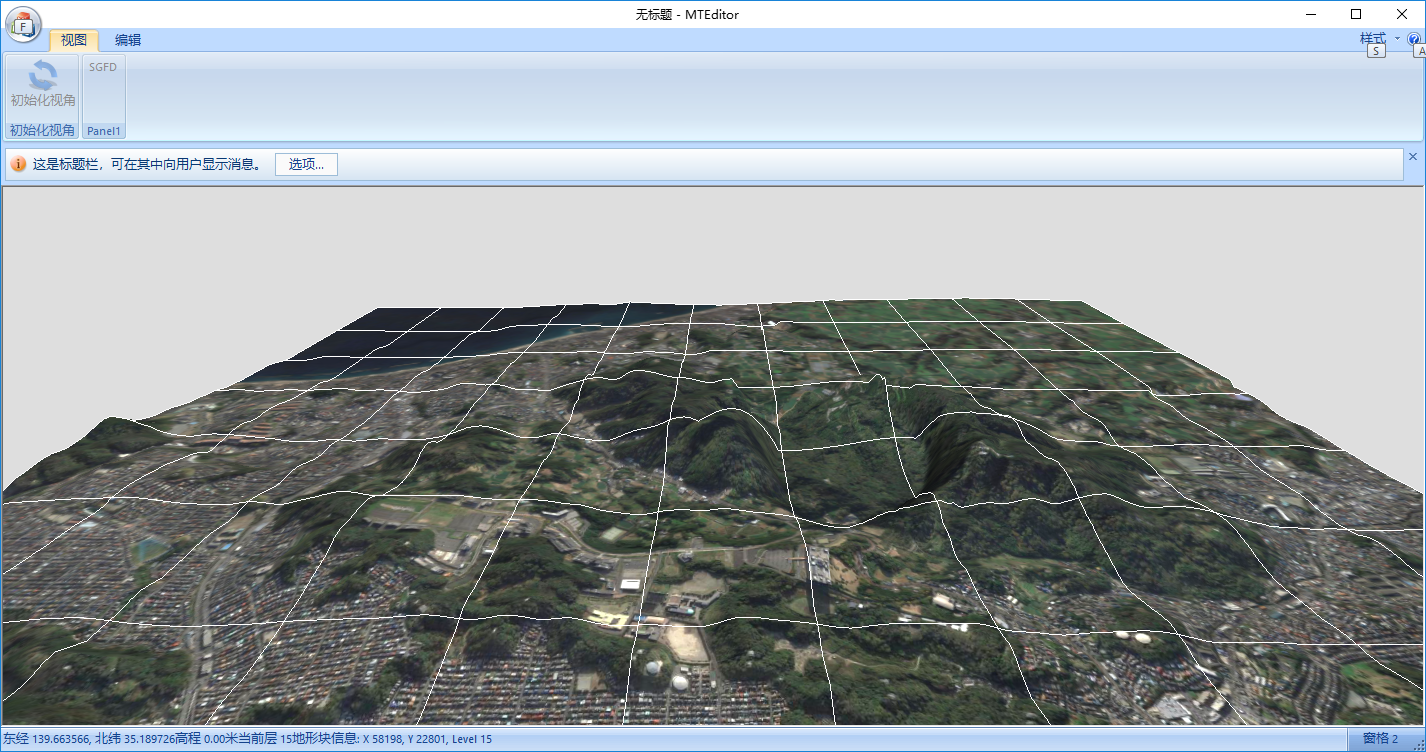
\includegraphics[height=4.2cm        ,width=7.2cm]{doc/example-utf8/figures/old.png}
\caption{VIWO系统中旧编辑器编辑状态效果}
\end{figure}
图4.6展示了本编辑器笔刷编辑的效果,图4.7展示了本编辑器中以选区方式进行地形平滑操作的过程,可以观察到选区边界的高程得到了良好的保持,且与选区区域内部过渡自然。旧地形编辑器中不具备地形选区的概念,当进行地形腐蚀操作时,直接对编辑范围内的地形进行操作,因此交互上可能会产生更大的延迟。完整的地形编辑效果详见附件。\par
\begin{figure}[h]
\centering
\subcaptionbox{}{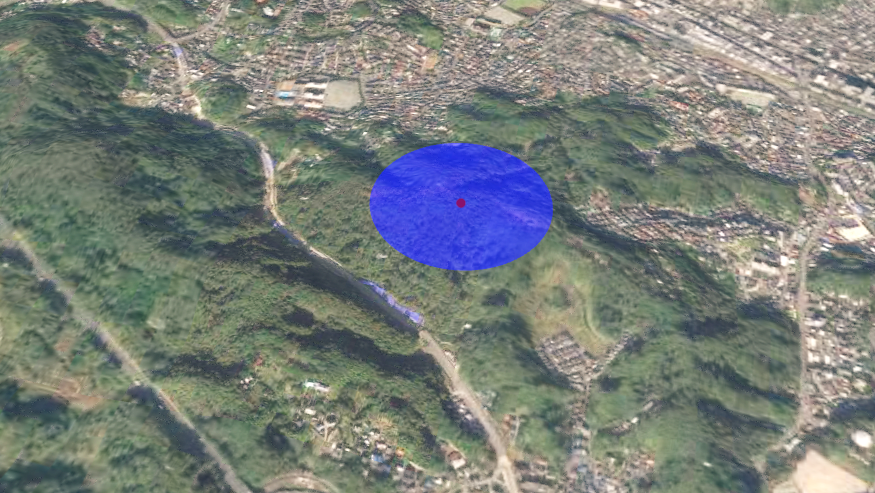
\includegraphics[height=3.5cm        ,width=6.0cm]{doc/example-utf8/figures/heightBefore.png}}
\subcaptionbox{}{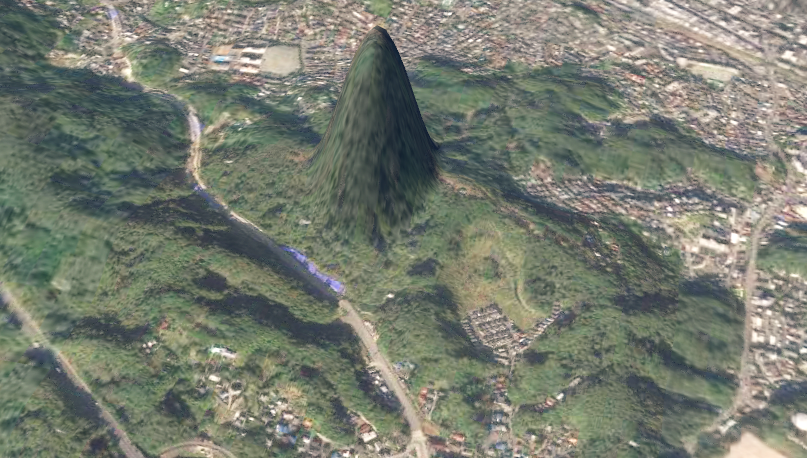
\includegraphics[height=3.5cm        ,width=6.0cm]{doc/example-utf8/figures/heightAfter.png}}
\caption{本编辑器实现的高程编辑效果(a).高程编辑前(b).高程编辑后}
\end{figure}

\begin{figure}[htbp]
\centering
\subcaptionbox{}{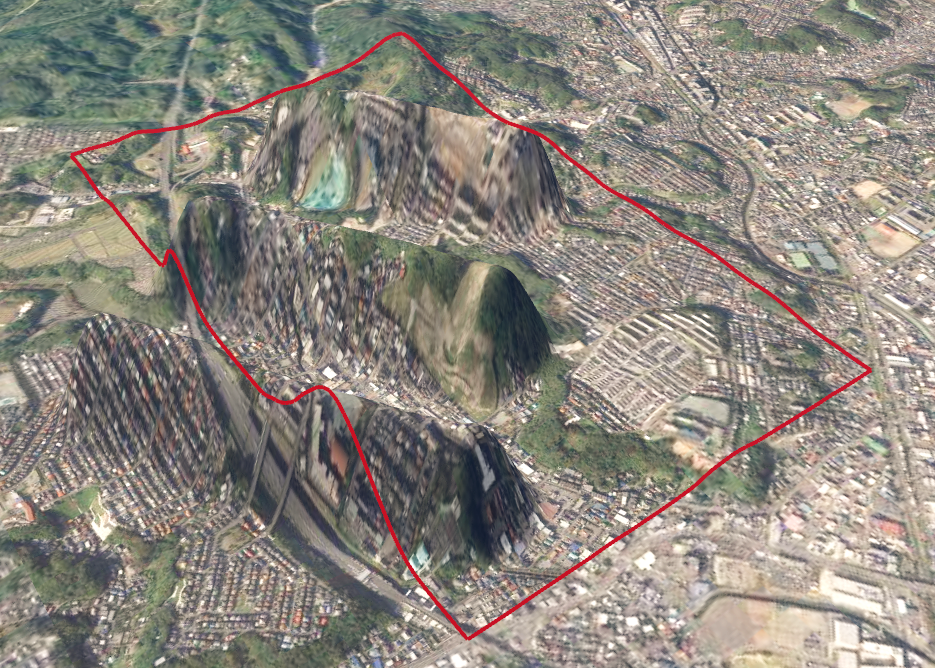
\includegraphics[height=3.5cm        ,width=6.8cm]{doc/example-utf8/figures/areaSmooth-.PNG}}
\subcaptionbox{}{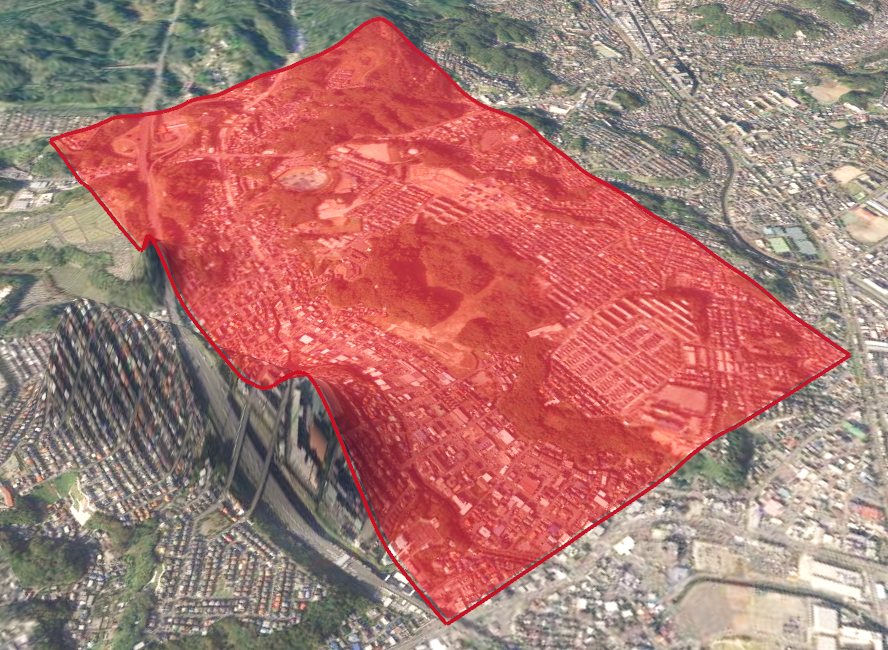
\includegraphics[height=3.5cm        ,width=6.8cm]{doc/example-utf8/figures/areaSmooth-2.PNG}}\\
%\subcaptionbox{}{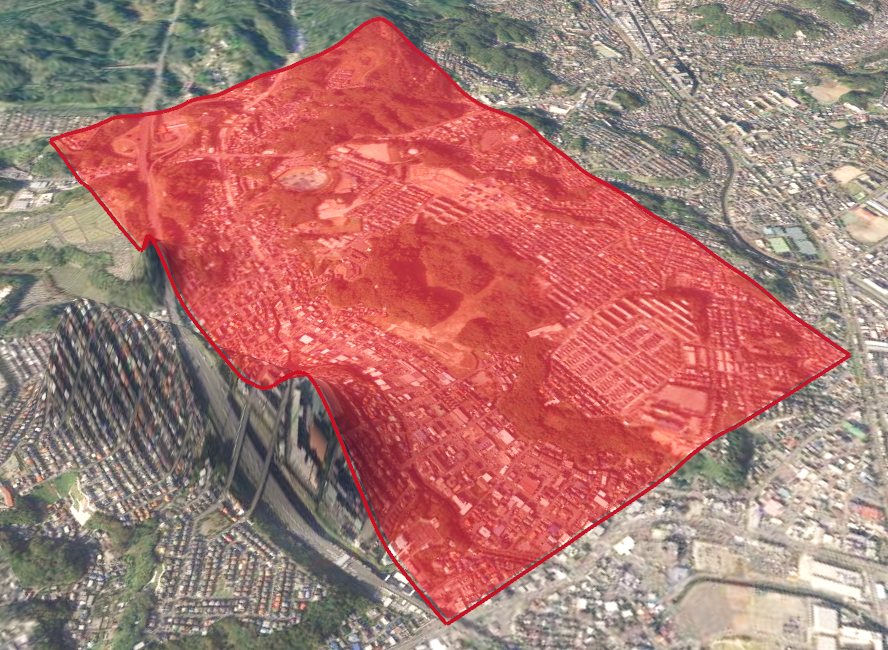
\includegraphics[height=4.5cm        %,width=7.2cm]{doc/example-utf8/figures/areaSmooth-2.PNG}}

\caption{在两种不同视角下对地形平滑结果的观察:(a).平滑前,可以看到选区中三条笔刷绘制出的山脉(b).平滑后}
\end{figure}

北京国遥新天地公司研发的EV-Globe6.0系统\supercite{ev-globe}是目前较为活跃的基于地形金字塔提供地形编辑功能的地形系统,其实现的高程画刷编辑效果如图4.8所示,可与本编辑器的实现效果进行对比。本编辑器的画刷渲染了画刷中心点,对用户的提示效果更明确,地形升降的效果上,两个系统基本相同。在地形平整功能上,EV-Globe6.0采用了矢量线编辑,编辑出的梯田地形边缘清晰,没有锯齿效果,但棱角较锐利。本编辑器对平整边缘的平滑使平整区域和未平整区域的过渡更加自然。
\begin{figure}[h]
\centering
\subcaptionbox{}{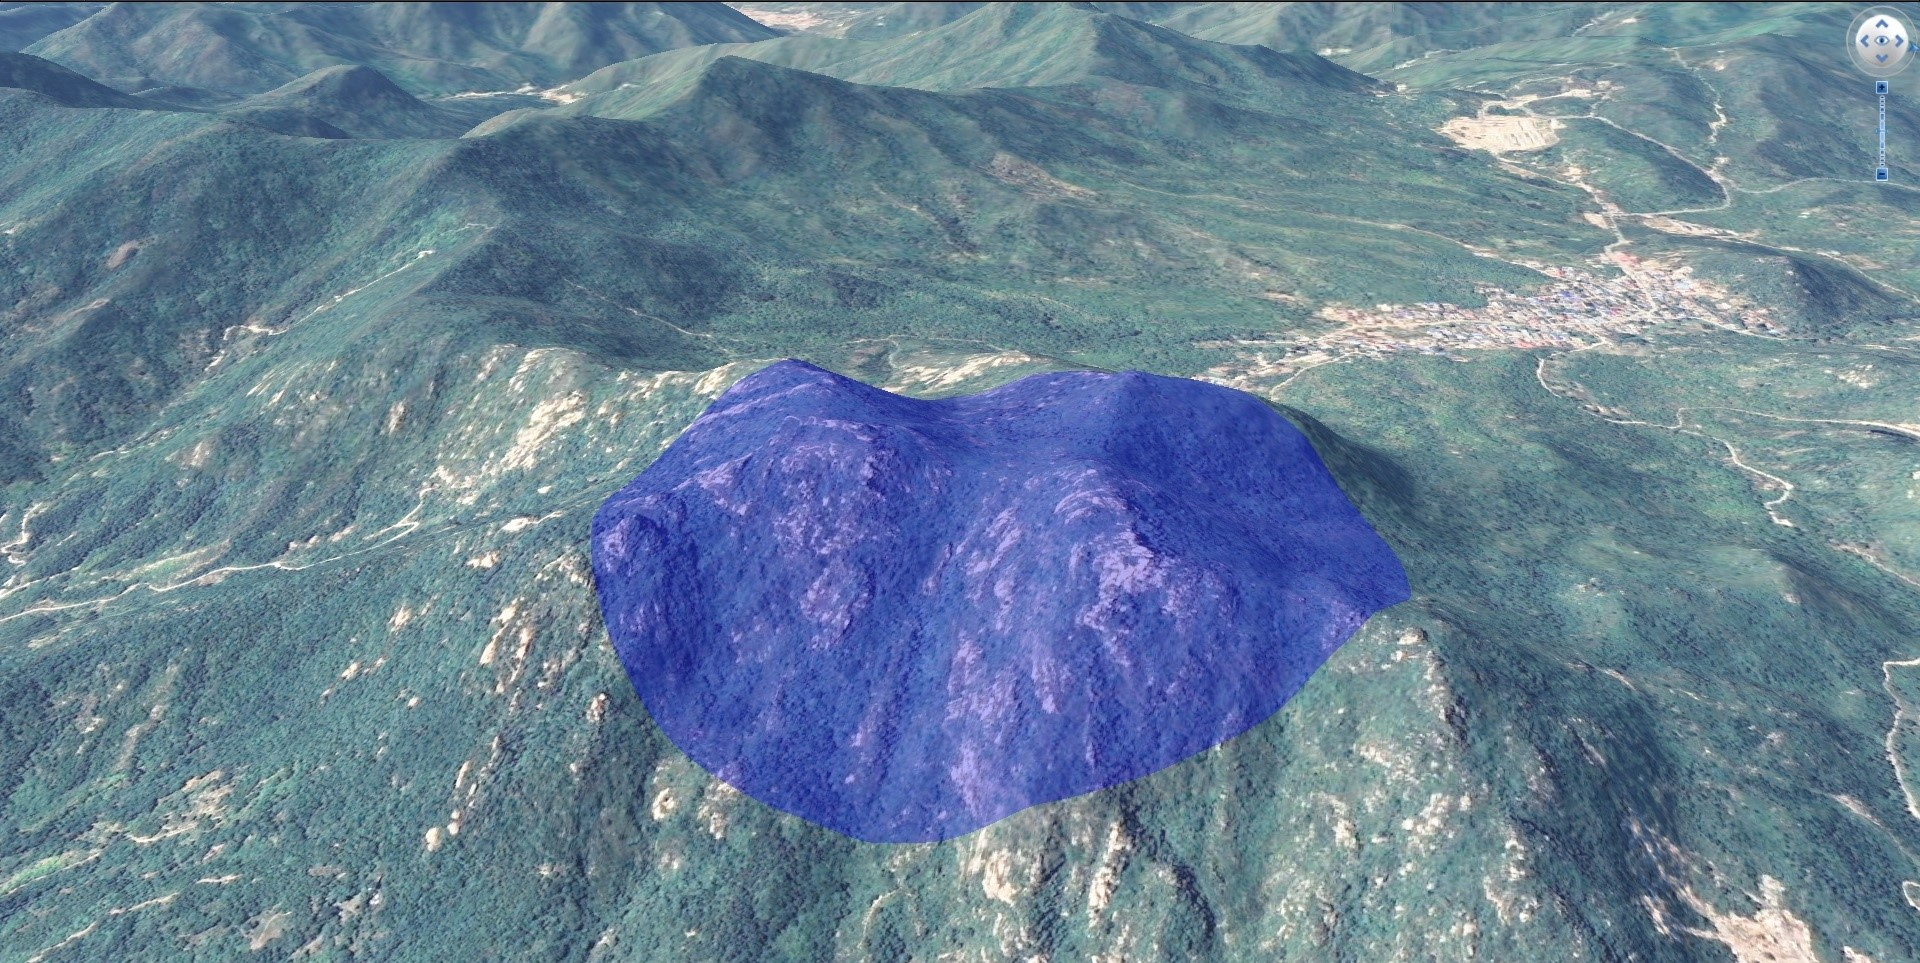
\includegraphics[height=3.5cm        ,width=6.7cm]{doc/example-utf8/figures/demBefore.jpg}}
\subcaptionbox{}{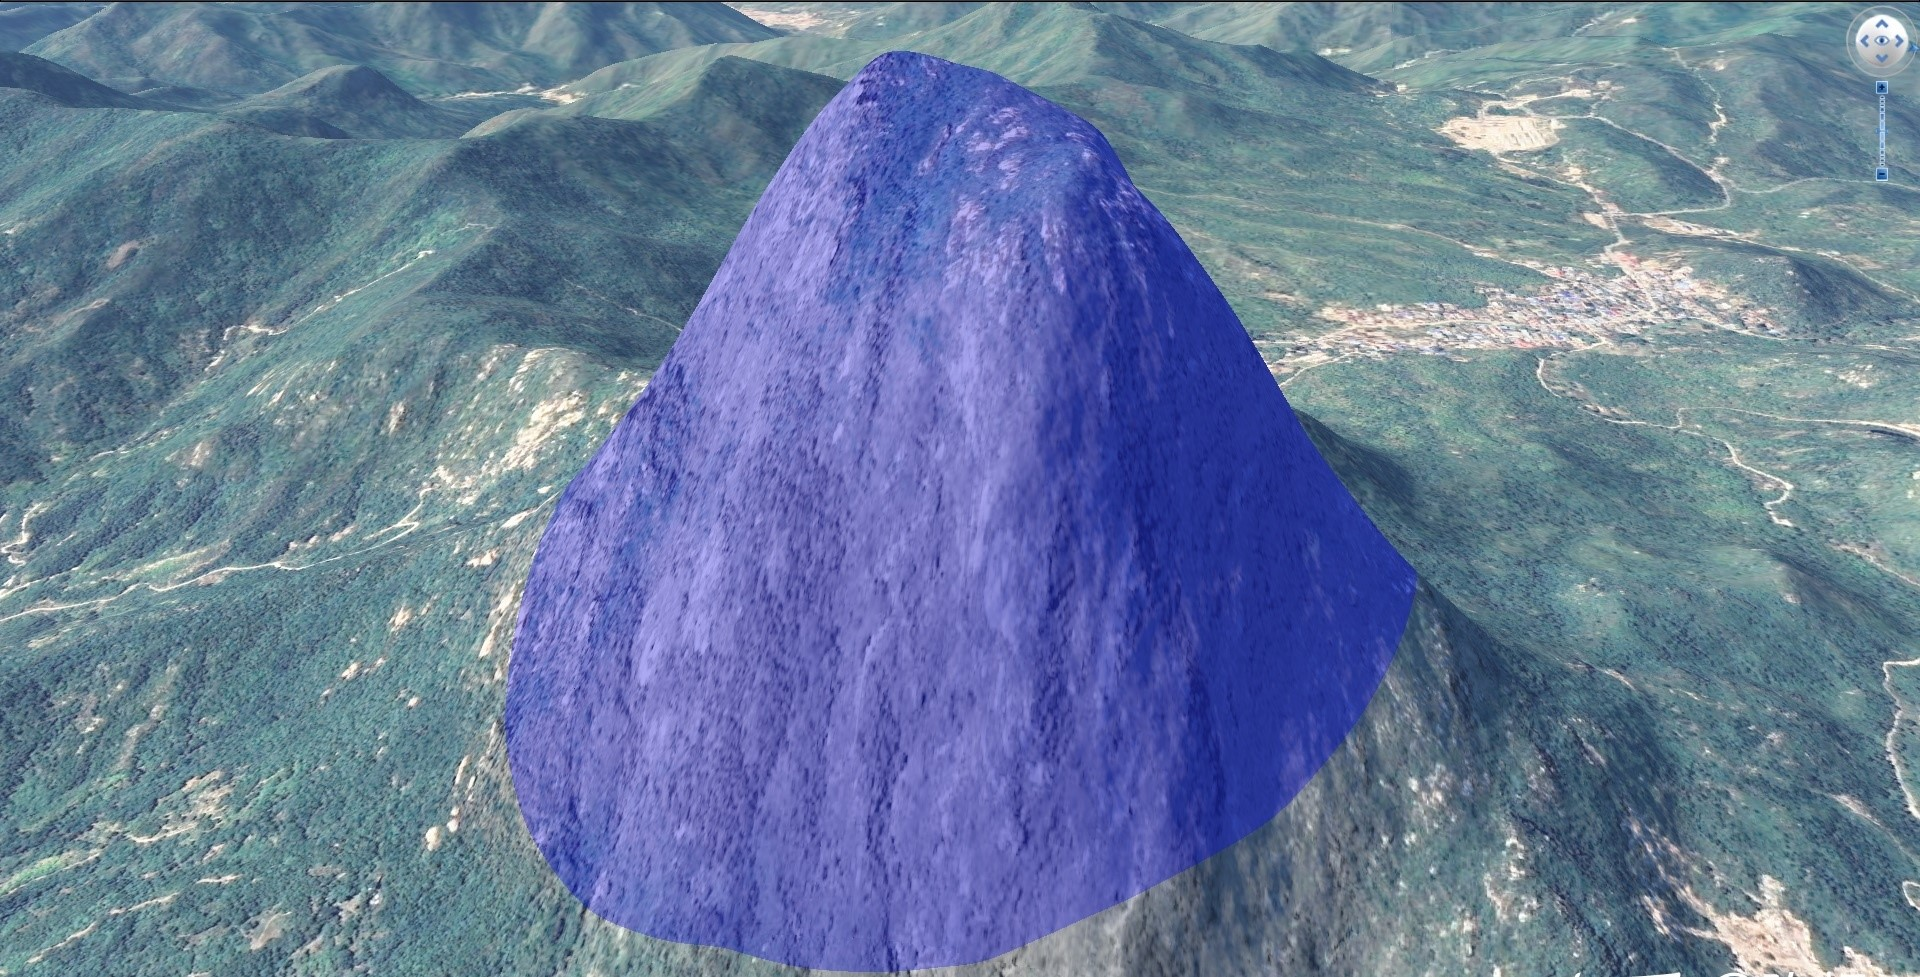
\includegraphics[height=3.5cm        ,width=6.7cm]{doc/example-utf8/figures/demAfter.jpg}}
\subcaptionbox{}{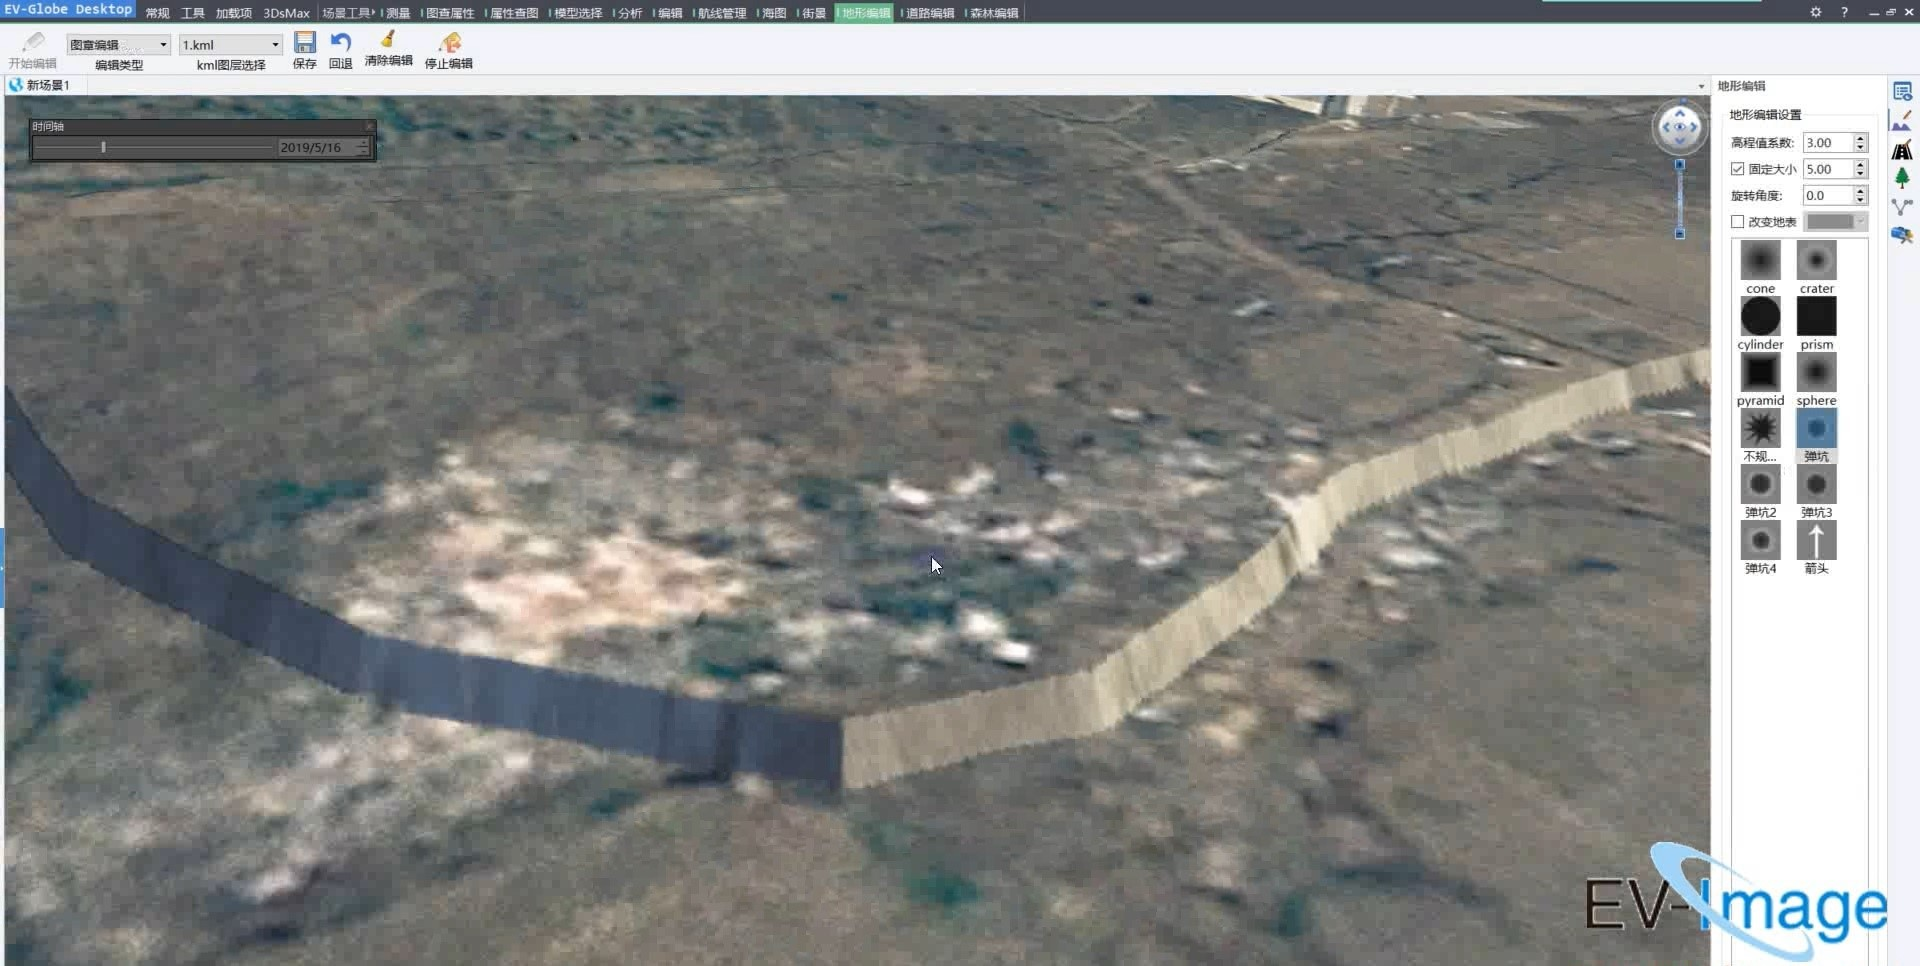
\includegraphics[height=4.2cm        ,width=7.3cm]{doc/example-utf8/figures/flattenEv.jpg}}
\subcaptionbox{}{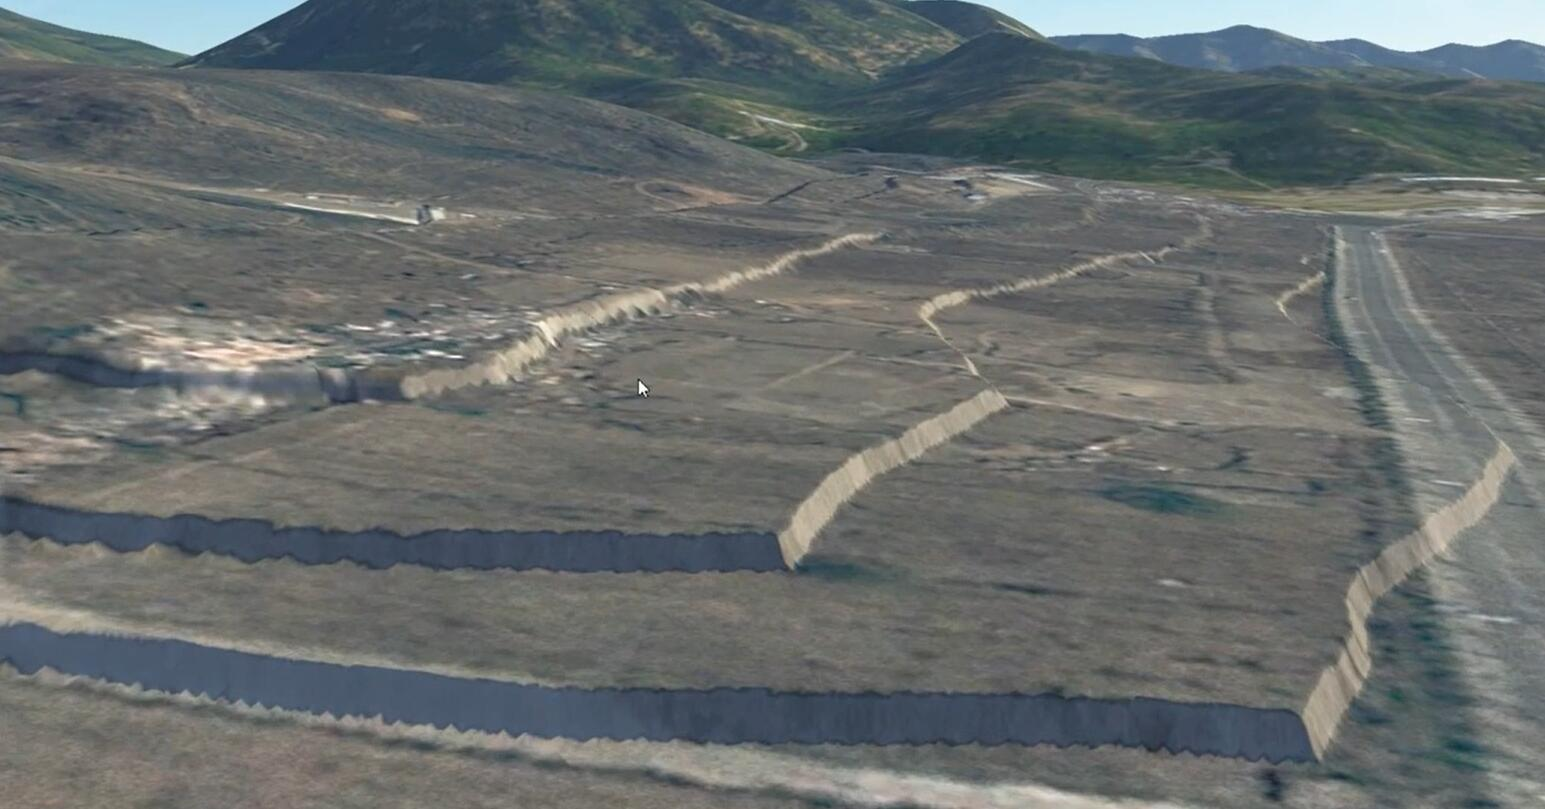
\includegraphics[height=4.2cm        ,width=7.0cm]{doc/example-utf8/figures/titianEv.jpg}}

\caption{EV-Globe6.0中的地形编辑器效果\supercite{ev-globe}:(a).高程编辑前(b).高程编辑后(c).平整编辑后(d).平整编辑构造的梯田场景}
\end{figure}
\section{本章小结}
本章介绍了编辑器中实现地形高程编辑的方法,包括使用笔刷和选区两种工具对地形进行平整、平滑等操作的算法。其中详细阐述了笔刷和选区编辑范围的确定,编辑结果的计算方法,并给出了实验结果。\par

% vim:ts=4:sw=4

 	\cleardoublepage
    % Copyright (c) 2014,2016,2018 Casper Ti. Vector
% Public domain.
\chapter{地形纹理编辑及纹理效果增强}
对于地形纹理编辑,较为直观的交互方式是使用笔刷对地表纹理进行绘制,通过多种材质叠加表达地形语义信息,丰富地表细节。本文利用纹理Splatting技术\supercite{splatting}进行纹理融合,这种技术使用透明度贴图将多种纹理融合到模型表面。这种纹理生成方式通用性强、效率高、资源占用较小且易于修改和编辑。由于地表纹理原先使用的卫星影像分辨率较低,而进行纹理编辑时可以为材质选择分辨率较高的素材,因此纹理编辑可以极大的提升近地漫游时地表纹理的清晰度,如图5.1所示。在此基础上,用户往往通过希望尽可能少且模糊的编辑操作实现内容丰富的地表纹理表达,对地表纹理的编辑结果添加一些过程式的修改能满足这种需求,对效果产生很大改进。对于卫星影像精细度低、承载内容有限等不足,本文还实现了纹理细节和纹理内容增强方法,以较低的资源占用率增加地表纹理的真实感。\par
\begin{figure}[htbp]
\centering
\subcaptionbox{}{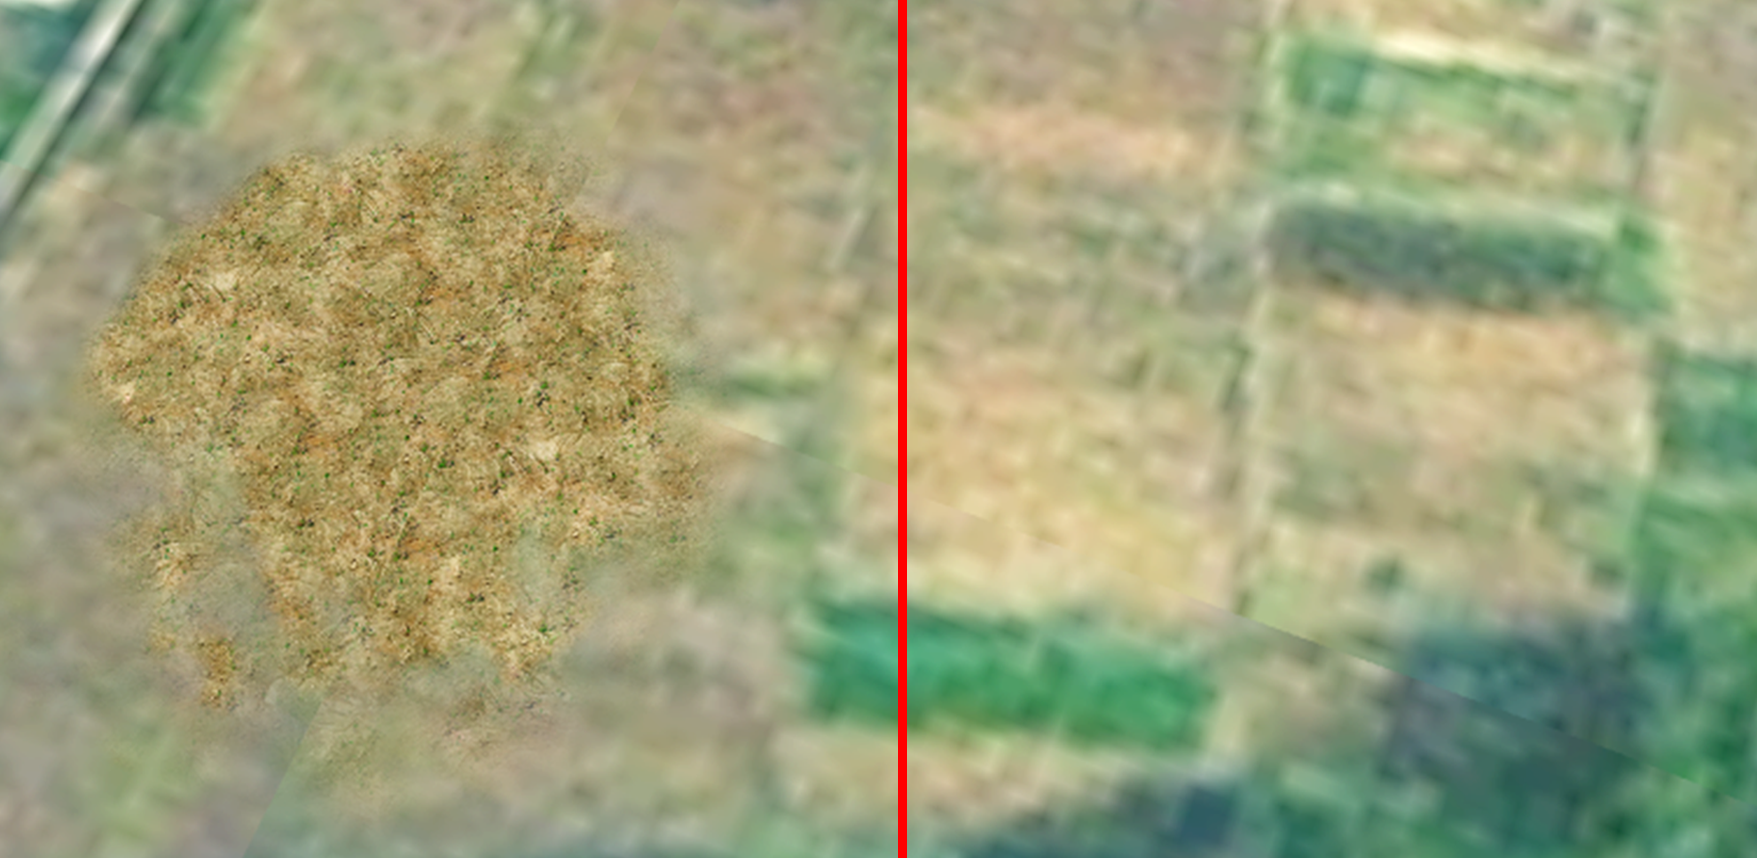
\includegraphics[height=3.3cm,width=6.3cm]{figures/groundComp.png}}
    \subcaptionbox{}{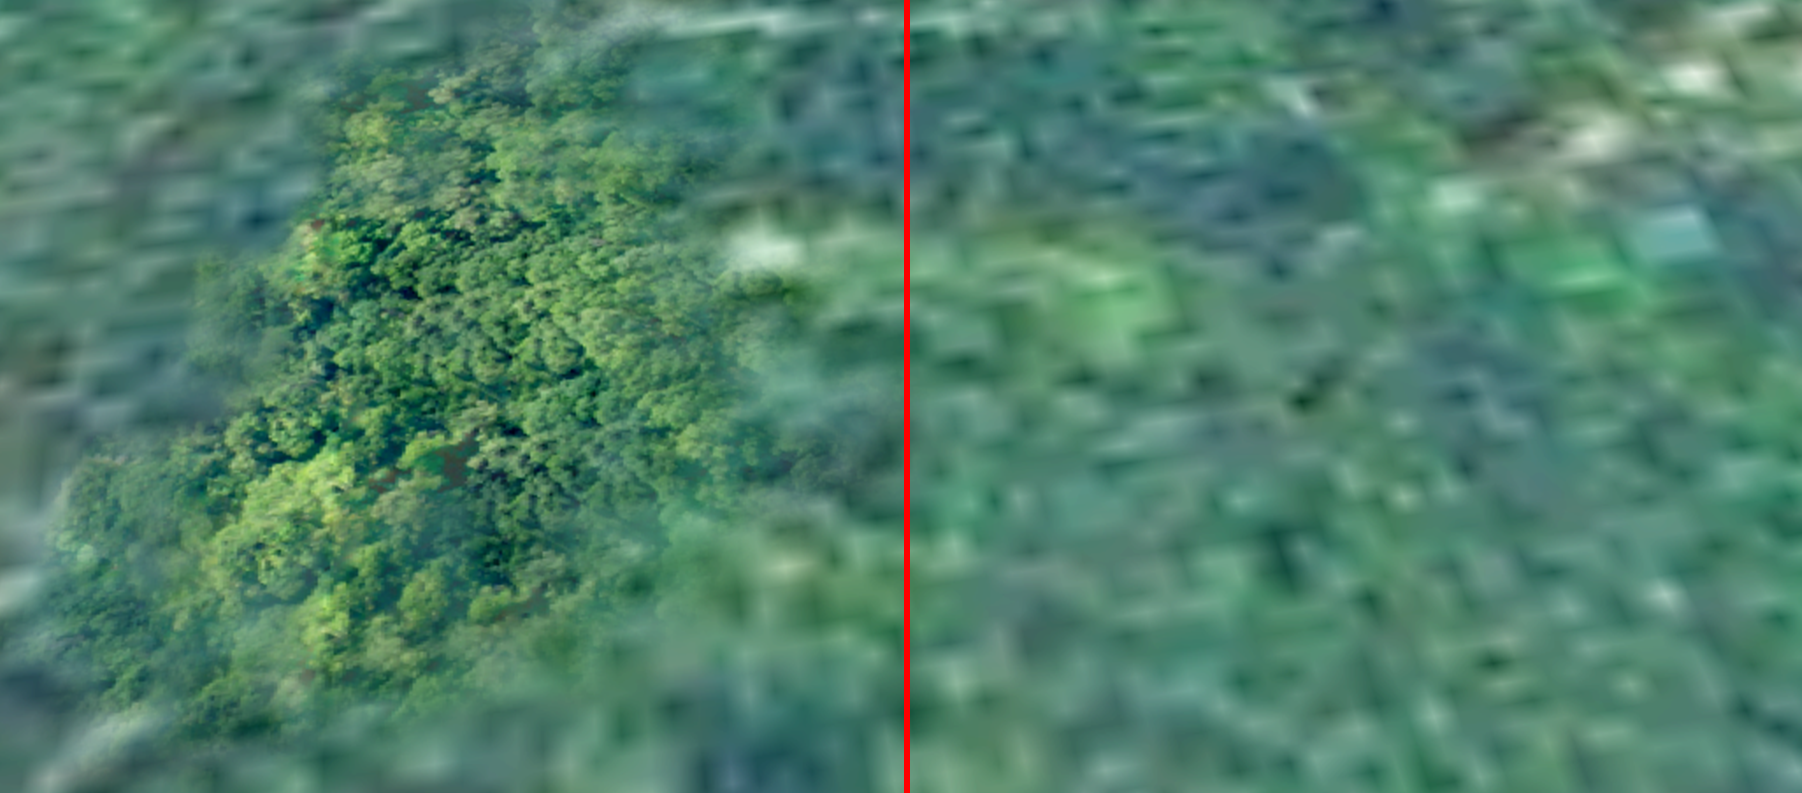
\includegraphics[height=3.3cm,width=6.3cm]{figures/treecomp2.png}}
\caption{纹理编辑可以提升地表纹理精细度:(a).纹理编辑结果与卫星影像中的田地效果对比(b).纹理编辑结果与卫星影像中的林地效果对比}
\end{figure}

\section{基于笔刷的纹理编辑}
本编辑器中,纹理材质来自人工挑选制作的无缝平铺贴图,透明度贴图则通过绘制生成,并称为\textit{蒙版}。有多种纹理材质参与编辑,其纹理混合结果按顺序叠加显示,因此以\textit{图层}的概念对多种纹理材质的编辑进行管理,每个图层使用一个材质。在GPU中将多种纹理材质按照蒙版提供的透明度融合后,将颜色叠加到地形纹理的颜色上。本节介绍基于笔刷生成蒙版数据的方法及蒙版数据的管理。

\subsection{栅格化笔刷应用策略}
笔刷数据由函数计算得到,其值域在$[0.0,1.0]$之间,表示该像素上笔刷的作用强度,以一维数组方式存储,但看作宽高相等的二维数组。编辑时,笔刷数据与蒙版数据中的像素是一一对应关系,如笔刷直径为$n$,则笔刷投影到蒙版数据上,覆盖$n*n$的像素,对此范围内的像素产生编辑效果。需要注意的是,由于地球经线在两极处收拢,因此纬线间距离相等而经线间距离不定。在计算笔刷数据时,为了在全球各个位置保持笔刷形状固定,需要根据笔刷的宽度和笔刷所在经纬度,对笔刷的高度进行校正。取笔刷所在地形块的四个角点,计算其全球坐标,将地形块宽高比作为笔刷的宽高比,然后进行笔刷数据计算。\par

与高程编辑笔刷不同,纹理笔刷是栅格化的,与纹理蒙版像素相对应,如图5.2所示。因此相机视角变换时,地形四叉树改变造成地形块层级变换,笔刷的覆盖面积也会随纹理蒙版数据分辨率的增加而变小,产生跳变。为保证笔刷大小的统一性,避免笔刷在换层时跳变,在系统中按固定层级渲染笔刷,该层级记为$L_r$。用固定层级渲染笔刷,保证了笔刷的渲染和其直径的调整在任意视角、任意层级上都连续,但编辑时还需使笔刷层级与当前编辑层级相一致。用两个一维数组存储用于渲染和用于编辑的笔刷数据,分别记为$B_r$和$B_e$,并分别提供获取和设置该数据的接口。当将笔刷渲染到画面中的地形表面时,根据笔刷直径和当前选中的笔刷的序号实时计算出用于渲染的笔刷数据$B_r$。而将笔刷数据用于编辑时,首先获取编辑层级,即当前地形四叉树中最精细的层级,记为$L_e$,按$L_e/L_r$的比例对笔刷直径进行缩放后再计算笔刷数据,保证编辑使用的笔刷数据与渲染使用的笔刷数据覆盖的面积大小相同。\par
\begin{figure}[htb]
    \centering
    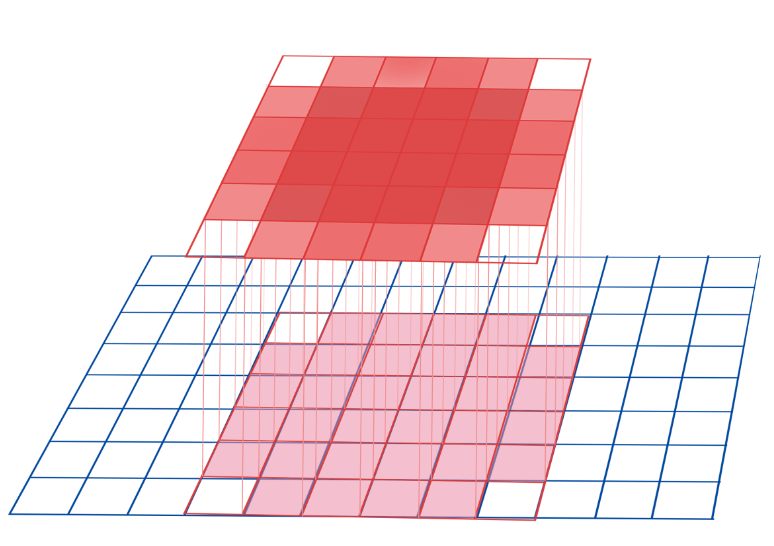
\includegraphics[height=4cm ,width=4cm]{figures/brush2.png}
  \caption{笔刷数据和蒙版数据像素一一对应}
  \end{figure}
%\begin{figure}[htb]
 %   \centering
 %   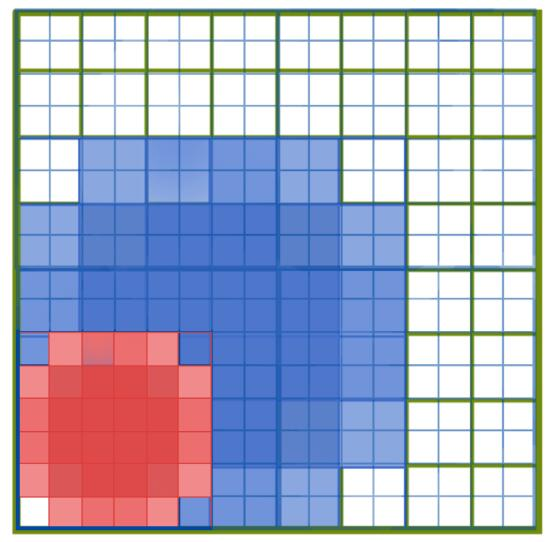
\includegraphics[height=5cm %,width=5cm]{figures/brushChange.jpg}
 % \caption{地形块换层时产生的笔刷跳变}
 % \end{figure}
  %
目前系统中地形四叉树的最高分裂层级为17层,记为$L_m$,笔刷渲染层级$L_r$为14层,考虑到计算笔刷编辑数据时对笔刷直径的调整,笔刷数据数组的宽和高(记为$n_{array}$)和可设置的最大笔刷直径(记为$n_{max}$)有如下关系:
\begin{equation}
n_{array}=(L_m/L_r)*n_{max}
\end{equation}
则存储笔刷数据的一维数组大小为$n_{array}*n_{array}$,并将其看作一个长宽均为$n_{array}$的二维数组,根据笔刷直径大小和当前选中的笔刷ID计算笔刷数据。\par
\subsection{蒙版及图层管理}
纹理编辑效果的呈现涉及图层信息和指导纹理材质混合的蒙版信息。图层信息与用户界面、配置文件等多个其他部分关系密切,因此设计为全局变量。蒙版信息与地形高程数据和纹理数据等价,是与地形块一一对应的,并以相同的方式管理和调度,挂载在四叉树的地形块节点内。\par
每个蒙版数据块内分别为每个图层提供一个数据分辨率与地表纹理数据相同的数组,该数组以智能指针进行管理,数组内每个图层的数据也以智能指针的形式管理,请求到某个图层时才为其分配内存。蒙版数据可能由父节点赋给其子节点临时使用,使用智能指针避免了内存无法正确释放的问题。蒙版数据内的像素都与地表纹理数据中的像素一一对应,每个图层在每个像素的位置用一个字节存储一个取值范围为$[0,255]$的整数值,表示该像素上对应图层的纹理材质参与颜色混合的强度,绘制时以纹理数组的形式发送给GPU。\par
图层信息包括图层名和图层使用的纹理材质。编辑器为载入的每种纹理材质生成唯一的纹理ID作为句柄,对于简单材质和复合材质是无差别的。用户界面也通过记录纹理材质选项的纹理ID,将用户所选择的纹理赋给图层。绘制时,图层所使用的纹理材质以纹理数组的形式发送给GPU,并在用户改动图层信息后设置脏标识,以向GPU传递新的纹理材质。目前系统最多允许八个图层,即可以同时使用八种纹理材质进行绘制。\par
编辑过程中有时由于调整了编辑意图,会需要抛弃整个图层的编辑结果,对图层进行删除是一种很自然的操作。删除图层涉及对多个部分数据的修改:在图层管理器中,需要将后面的图层依次前移覆盖待删除图层信息,并更新用户界面;在过滤器中,需要删除基于该图层的补丁数据;对LRU缓存中的全部蒙版缓存块,需要保留指向待删除图层蒙版数据的智能指针,将后面图层在数组中的位置前移,将待删除图层的指针放在前移后出现的空缺处。
%由于删除图层后需要向GPU传递这种更新,因此不能释放被删除图层的内存,而需要将其重置为0。
\subsection{复合纹理材质}
目前系统中的海面由高程值为0的均匀四边形面片绘制,通过噪声计算对网格点进行偏移形成海洋波浪效果。而内陆的水体如河流、湖泊等,是通过编辑工具改变地形高程值,使地形高度低于海平面,暴露出海洋网格而产生的。这种实现方式存在几个问题:(1)编辑工具产生一条折线作为河道中心线,对地形高程进行修改,产生的河道是等宽的,效果较为僵硬、不自然,尤其在河道中心线发生大角度转折时容易产生断裂;(2)距离较远观看时由于数据分辨率问题,河岸产生非常大的锯齿效果;(3)这种方法无法表现存在高度变化的水体,如从沿着山体坡度流下的河流,或高原湖泊等。图5.3示意了上述的三个问题。
\begin{figure}[htb]
    \centering
    \subcaptionbox{}{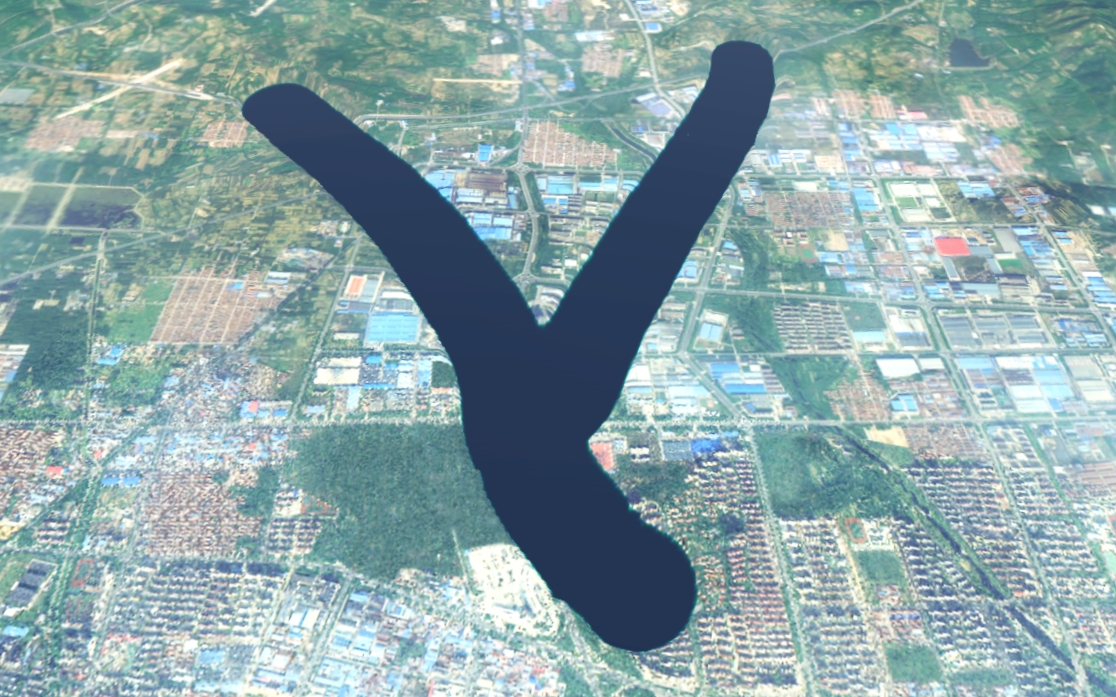
\includegraphics[height=3.7cm,width=5.3cm]{figures/riverLow.PNG}}
    \subcaptionbox{}{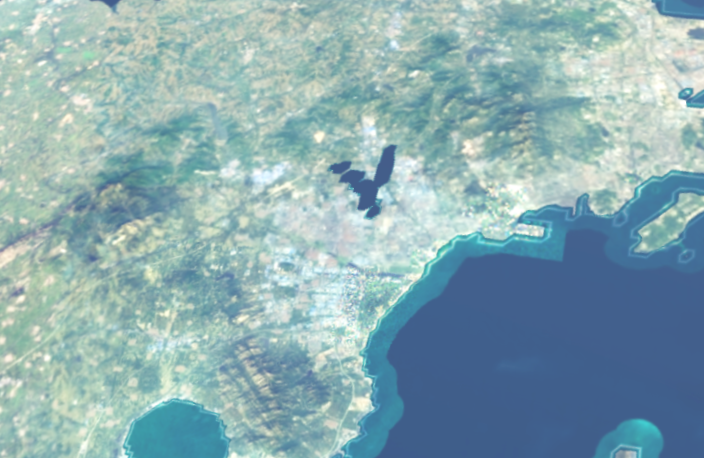
\includegraphics[height=3.7cm,width=5.3cm]{figures/riverHigh.PNG}}
    \caption{基于地形高程编辑实现的河流在高空视角出现严重的锯齿:(a).低空绘制并观察时没有锯齿(b).编辑结束后升高视角,出现严重锯齿}
\end{figure}
因此,用纹理编辑的方式对水体编辑进行改进成为了自然的想法。水体一个重要的视觉特性就是其对太阳光的高光反射。为使水体产生高光反射,需要向着色器中传入水面材质的法线信息,由此引出了构造复合材质的需求。\par
将只有颜色贴图的单一资源的纹理材质扩充为包含颜色贴图、法线贴图等资源的复合纹理材质,可以创建更复杂的地表纹理编辑效果。但只有颜色贴图的简单材质依然非常方便实用,复合材质和简单材质需要同时应用在系统中。在本地的配置文件中对复合材质所需的多种贴图资源路径进行配置,并在着色器中增加一个变量用于表示当前材质所包含的资源种类,以在着色器中同时对包含不同资源的纹理材质进行统一处理。以复合材质实现的内陆水体效果如图5.4所示:
\begin{figure}[htb]
    \centering
    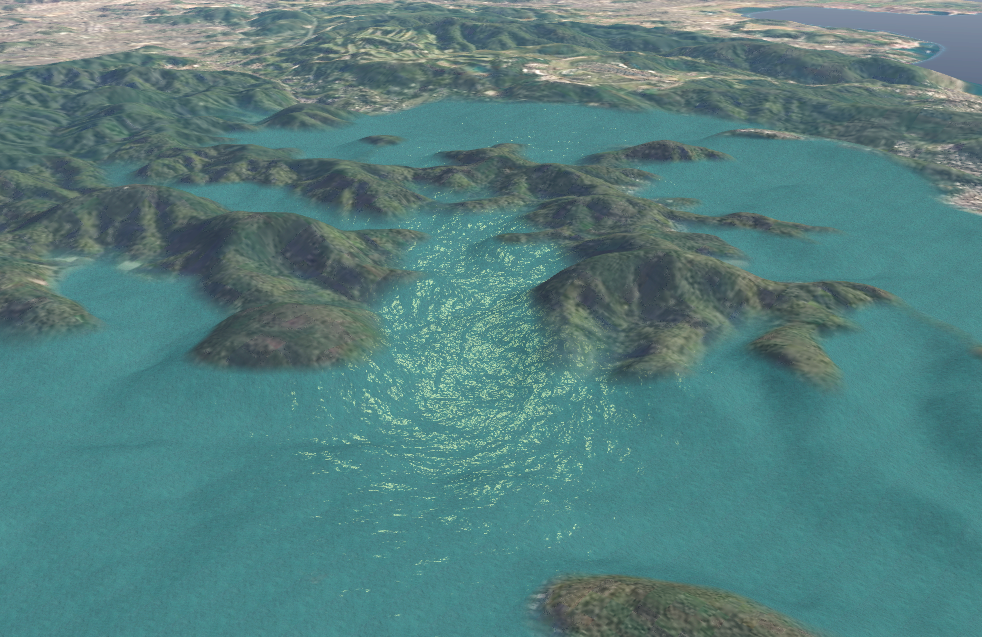
\includegraphics[height=6cm,width=9.4cm]{figures/water.png}
    \caption{复合材质和基于高程规则的纹理笔刷实现的内陆水体效果}
\end{figure}
\subsection{基于高程规则的过程式纹理笔刷}
积雪和植被等地物存在垂直分布规律,高程数据所表达出的地貌通常应与地面纹理表达的内容相对应。尽管受到地理位置和气候等因素影响,且不同地形的垂直分布存在差异,但总的来说积雪、植被等地物分布呈现一定规律。基于对自然界地景规律的观察,用地形的海拔高度、斜率等数据作为笔刷编辑的辅助约束成为了很自然的想法。\par
将对笔刷编辑结果的约束条件称为\textit{过程式编辑规则},需要在配置文件设置的参数包括过程式编辑规则的名称、地形高度、地形斜率、过渡带宽度等。进行笔刷编辑时,如未选中过程式编辑规则或处在橡皮擦模式,则不做处理。当选中过程式编辑规则时,编辑曲线绘制工具在创建纹理蒙版补丁数据的同时,还需要创建一块等大的高程补丁数据,并拷贝原始高程数据进行填充。同时由于该过程式编辑规则只应用在单条笔迹上,不能对整个地形块蒙版数据的其他部分产生影响,需要将本次编辑的笔迹与之前的编辑痕迹区分开,因此还需要创建一块等大的空白的补丁数据,用于接受本次的编辑结果。\par
首先,按照原有的编辑流程通过笔刷绘制点和笔刷模板生成编辑结果。对于不应用过程式编辑规则的编辑笔迹,直接修改到蒙版补丁数据上,对于应用过程式编辑规则的编辑笔迹,则先修改到空白补丁数据上。与高程编辑不同,纹理编辑的笔刷编辑结果计算无需采样现有的数据,笔迹之间编辑效果是独立的,因此可以保证先将编辑结果应用到空白补丁数据上,再合并回蒙版补丁数据的正确性。当一条笔迹绘制结束时,在将编辑结果向各地形块数据分发之前,首先对编辑出的补丁数据应用过程式编辑规则。将编辑生成的补丁数据和高程补丁数据传输到GPU端,类似地形选区编辑,将补丁数据渲染到一个四边形面片上,在片元着色器中应用过程式编辑规则。对于补丁数据中的每一个像素,其初始透明度为1.0,按顺序应用过程式编辑规则中的多个约束条件,如高程约束、斜率约束等,每个约束条件依次对透明度值进行修改。过渡带在高程约束计算中的应用如图5.5所示,红色的两条线表示用户自定义配置的高度上限和下限,橙色线表示过渡带上边界和下边界,红色和橙色线间的部分表示过渡带,其宽度也由用户定义,过渡带可以使编辑结果不会出现硬边界。
\begin{figure}[H]
    \centering
    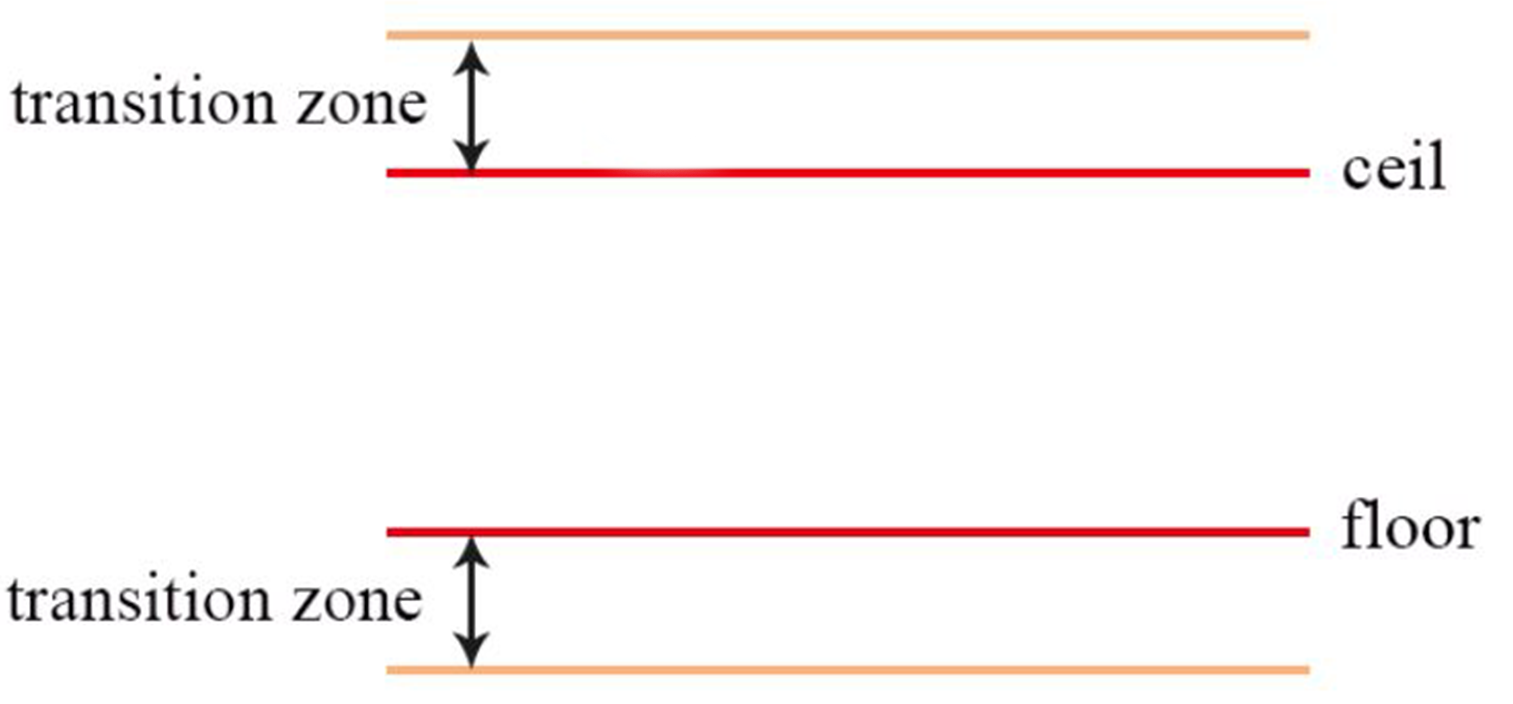
\includegraphics[height=3.4cm ,width=6.3cm]{figures/trans.png}
    \caption{高程规则的计算}
 \end{figure}
应用过程式高程规则的算法如下所示:\par
 \begin{algorithm}[H]
	\renewcommand{\algorithmicrequire}{\textbf{Input:}}
	\renewcommand{\algorithmicensure}{\textbf{Output:}}
	\caption{过程式高程规则应用算法}
	\label{alg:1}
	\begin{algorithmic}[1]
		\REQUIRE 地形高程$H$,地形斜率$G$,高程规则$R_h$,斜率规则$R_g$,过渡带宽度$T$,过渡带硬度$S$,算法强度$I$
		\ENSURE 蒙版补丁数据透明度$opacity$
		\STATE 设置$opacity$为1.0
	    \IF {$H$ > $(R_h.ceil+R_h.floor)/2$}
	    \STATE 设置$opacity$为$opacity$与$(R_h.ceil+T-M_d)/(T*S)$的乘积,并截取在[0.0,1.0]之间
	    \ELSE
	    \STATE 设置$opacity$为$opacity$与$(M_d-R_h.floor+T)/(T*S)$的乘积,并截取在[0.0,1.0]之间
		\ENDIF
		\IF {$G$ > $R_g.floor$且$G$ < $R_g.ceil$}
	    \STATE 设置$opacity$为$opacity$与1.0的乘积
	    \ELSE
	    \STATE 设置$opacity$为$opacity$与$(1-I)$的乘积
		\ENDIF
		\STATE \textbf{return} $opacity$
	\end{algorithmic}
\end{algorithm}
图5.6和5.7展示了上述算法的应用效果:
\begin{figure}[H]
    \centering
   \subcaptionbox{}{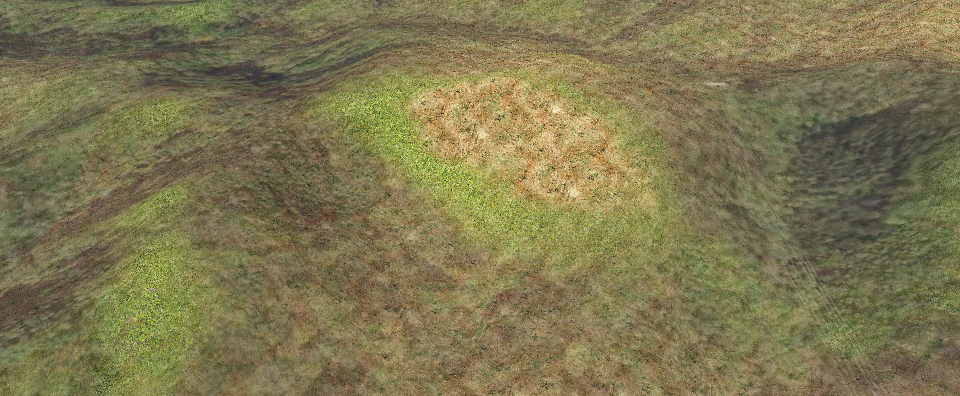
\includegraphics[height=4cm,width=5.5cm]{figures/gradient2.PNG}}
   \subcaptionbox{}{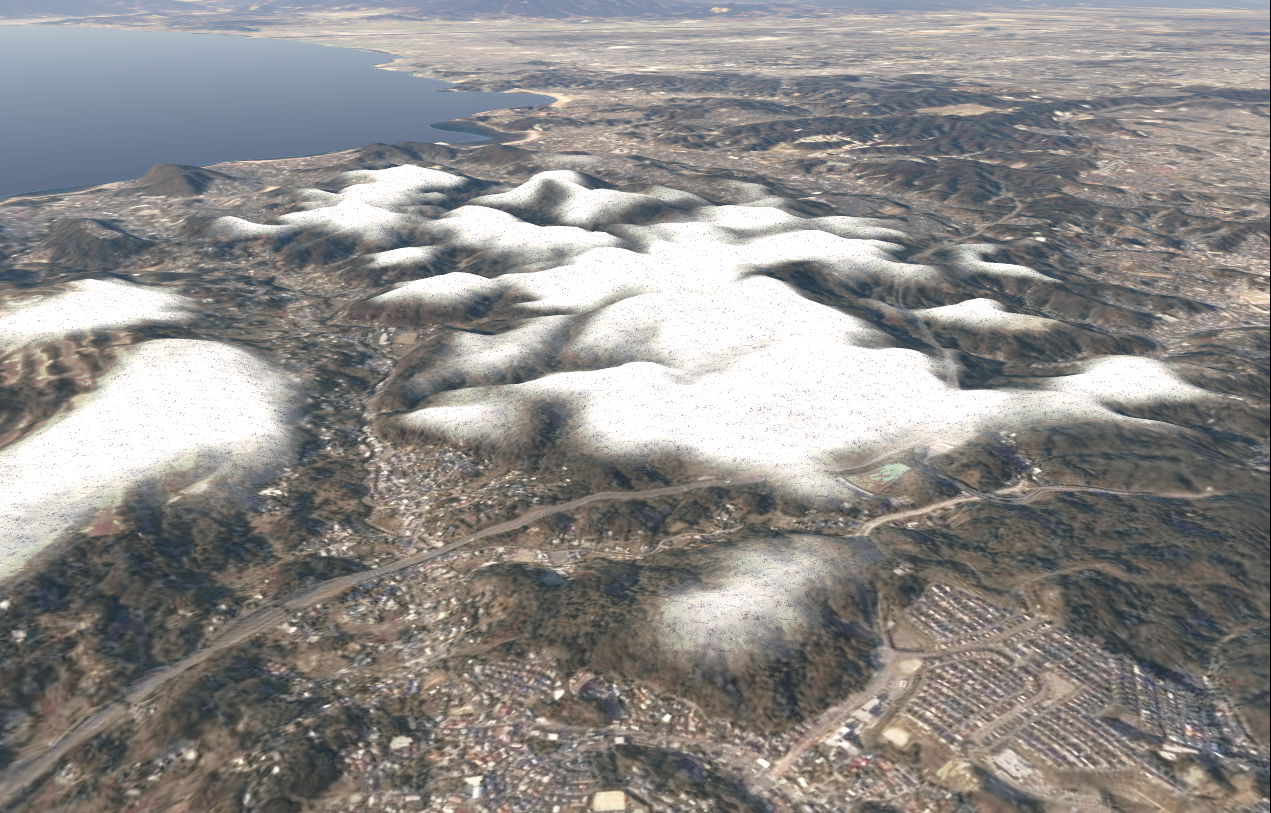
\includegraphics[height=4cm,width=5.5cm]{figures/pc-snow.png}}
  \caption{使用过程式编辑规则的纹理笔刷效果:(a).通过斜率约束绘制山坡陡峭处的地表裸露(b).通过高程约束和斜率约束实现山顶积雪效果}
\end{figure}

\begin{figure}[H]
    \centering
    \subcaptionbox{}{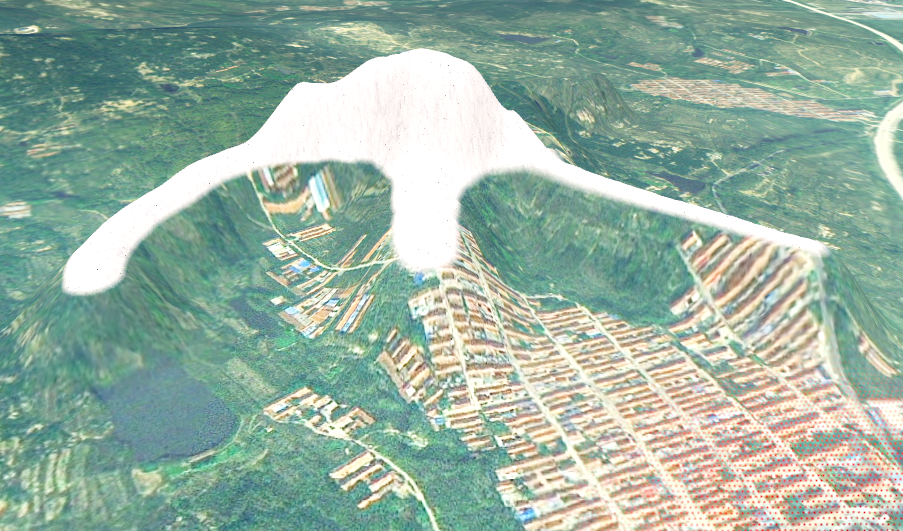
\includegraphics[height=3.2cm,width=5.2cm]{figures/110-0-35.PNG}}
    \subcaptionbox{}{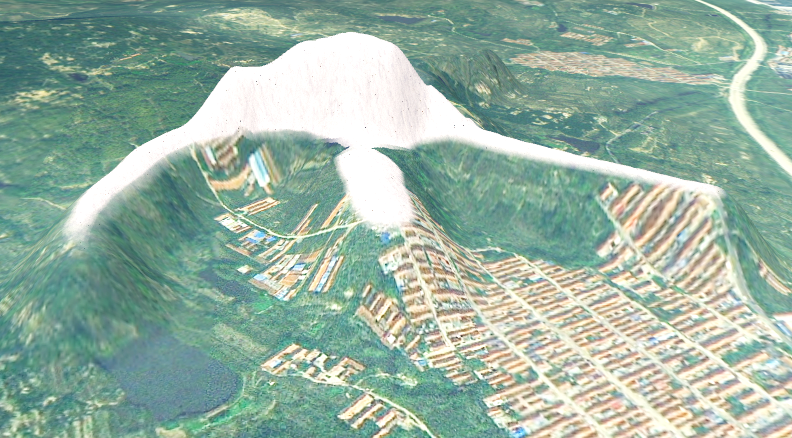
\includegraphics[height=3.2cm,width=5.2cm]{figures/110-0-19.PNG}}
    \subcaptionbox{}{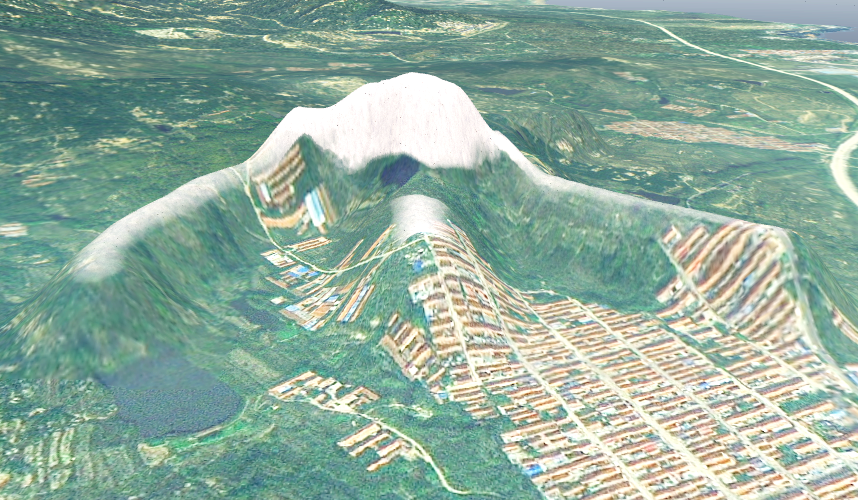
\includegraphics[height=3.2cm,width=5.2cm]{figures/110-0-13.PNG}}
    \caption{高程规则参数调整效果:高程下限:110.0,斜率下限:0.0(a).斜率上限:13.0(b).斜率上限:19.0(c).斜率上限:35.0}
\end{figure}

\section{纹理细节增强}
目前ViWo系统使用的卫星数据是由日本METI和美国NASA联合研制的ASTER-GDEM-V2数据集,其水平精度为30米,垂直精度为20米。受数据精度限制,漫游视角靠近地表时纹理看起来非常模糊,若直接将建筑模型置于缺乏细节的地表上,近距离观看时真实感较差。本文参考Genesis\supercite{genesis}等飞行视景模拟器的近地表效果,实现了基于粗糙影像的纹理合成,对低分辨率的地表纹理的颜色信息进行分析,以贴花技术为地表纹理增添细节。本方法的有效性和可行性基于对以下三点的考虑:(1)颜色是在图像处理中应用最广泛的视觉特征值,颜色包含的信息往往与图像中物体或场景的语义信息十分相关;(2)相比其他视觉特征,颜色信息对图像本身的尺寸、方向、视角的依赖性较小,提取颜色信息进行语义分析具有较高的鲁棒性;(3)本方法在片元着色器中对片元颜色进行简单处理,时间及空间开销非常低。\par
对颜色信息进行分析时,在不同的色彩空间进行处理分析的效果不同。颜色可以用一维、二维、三维和四维空间坐标表示,定义颜色的色彩空间有很多种,常用的有RGB、CMYK、HSV等。RGB色彩空间的特点之一是其三个通道的数值都容易随图片亮度改变,使结果颜色的明暗发生变化,但色调并不会产生很大变化。而往往一个通道的轻微改变,会导致最后融合在一起的颜色发生很大变化。HSV色彩空间可以较好地把颜色信息和亮度信息分开,将它们放在不同的通道中,减小了光线强度对于特定颜色识别的影响,在图像处理领域很常用。但经过实际测试,由于可能为植被的区域跨越的色环角度较大,在HSV色彩空间进行阈值分割的效果不够好,因此本文选择在RGB色彩空间进行颜色分析。由于RGB色彩空间受颜色亮度影响强烈的特性,因此不能简单的基于RGB色彩空间中某个通道的固定阈值对颜色进行判断,但可以以红、绿、蓝三种光的相对占比作为衡量的标准之一。\par
虚拟地球漫游中用户比起海洋更加关注陆地区域,陆地区域中最关注的地形语义以城市和城市周边自然环境为主,其中自然环境以植被覆盖的地形和土地、荒地为主,城市地物以建筑屋顶、道路为主。本文实现中以森林绿、泥土棕、建筑灰三种颜色对上述三种区域进行语义分割,并在渲染时在相应区域添加对应的细节,基本可以满足对地表纹理的细化需求。算法的主要思想是检查片元颜色是否较强烈的指向某种语义。如果是,则完全的使用对应语义的贴花纹理,否则对多种贴花纹理进行混合。森林绿和建筑灰在语义上强烈的指向植被和建筑屋顶,可以认为有这样颜色的像素语义较为清晰。而其他颜色的像素可能是由于图像分辨率低和卫星影像阴影问题,导致语义较为模糊。选择具有普适性的泥土的细节纹理作为两个区域间的过渡,在不明确是植被也不明确是建筑的部分进行细节纹理的混合。需要注意的是,纹理编辑后对地表纹理的语义信息也施加了改变,在着色器中可以得到从卫星影像采样和纹理编辑结果叠加后的像素颜色,将该颜色用于判定。算法输入片元颜色,输出三种细节纹理的alpha值,作为进行细节纹理混合的依据,最后将细节纹理叠加到原有的片元颜色上。为使细节只在近地漫游时出现,该算法在高空视角和低空视角呈现差异,根据当前四叉树中的最精细层级对细节纹理的透明度进行调整。
算法详细流程如算法2所示,图5.8从高空视角展示了语义划分的结果,并从近地面视角展示了贴花应用结果。

\begin{algorithm}[h]
	\renewcommand{\algorithmicrequire}{\textbf{Input:}}
	\renewcommand{\algorithmicensure}{\textbf{Output:}}
	\caption{基于粗糙卫星影像的贴花纹理alpha值计算}
	\label{alg:1}
	\begin{algorithmic}[1]
		\REQUIRE 卫星影像采样颜色$C_s$,当前四叉树最精细层级$l$
		\ENSURE 植被细节纹理alpha值$A_g$,建筑细节纹理alpha值$A_b$,泥土细节纹理alpha值$A_s$,细节纹理总体alpha值$A_m$
		\STATE 设定细节纹理最小混合层级$l_{min}$和最大混合层级$l_{max}$,砖石颜色$C_b$,植被细节纹理阈值$t$,建筑细节纹理阈值$s$
		\STATE 将$A_m$设置为$l$-$l_{min}$的倍数,并截取其值在$[0.0,1.0]$
		\STATE 将$sum$设置为$C_s$三个通道值的和
		\STATE 将三元量$contrib$设为$C_s$三个分量与$sum$的比值
		\STATE 设置$A_g$为$contrib.g$的两倍并截取其值在$[0.0,1.0]$
		\STATE 设置$A_b$为$C_s$与$C_b$的点乘
	    \IF {$A_g$ > $t$}
	    \STATE 设置$A_g$为1,$A_b$、$A_s$为0
	    \ELSIF{$A_b$ > $s$}
	    \STATE 设置$A_b$为1,$A_g$、$A_s$为0
	    \ELSE
	    \STATE 设置$A_s$为1减去$A_g$和$A_b$结果的倍数
		\ENDIF
		\STATE \textbf{return} $A_g$, $A_b$, $A_s$
	\end{algorithmic}
\end{algorithm}
\begin{figure}[H]
    \centering
    \subcaptionbox{}{\includegraphics[height=4.3cm,width=6.4cm]{figures/origin-devide.png}}
    \subcaptionbox{}{\includegraphics[height=4.3cm,width=6.4cm]{figures/devide.png}}
    \subcaptionbox{}{\includegraphics[height=4.6cm,width=6.4cm]{figures/beforedecal.PNG}}
    \subcaptionbox{}{\includegraphics[height=4.6cm,width=6.4cm]{figures/afterdecal.png}}
    \caption{贴花技术应用结果:(a).原卫星影像(b).区域划分结果:绿色部分为植被,棕色部分为土地,灰色部分为建筑(c).应用贴花技术前,近地漫游时局部地表纹理非常模糊(d).贴花技术应用效果,图中可见植被、泥土和砖石不同的细节纹理}
\end{figure}
\section{卫星影像内容增强}
用卫星影像作为地表纹理构建虚拟地球存在一个局限,即卫星影像数据只能呈现特定季节的环境。对于飞行视景模拟等应用,用户希望能对多种环境进行模拟,对虚拟环境季节特征的体现是很自然的需求。从卫星影像的层面来看,季节变化过程中在图像中呈现最大变化的是植被覆盖的地区。因此对植被覆盖区域进行后处理可以很大程度的模拟不同季节的卫星影像。\par
ASTER-GDEM-V2数据集摄制于夏季,因此图片中颜色偏绿且明度低的部分很可能是植被覆盖的区域。春夏季的卫星影像特征是植被覆盖区域呈现深绿色,秋季则由于植被枯黄,在植被覆盖区域渐渐呈现土黄色、黄棕色。冬季的卫星影像特征是植被凋零,原有的绿色植被区域留下枝干和泥土,呈现深棕色。除此之外,冬季会出现积雪,覆盖除道路之外的大部分区域,真实的雪天卫星影像主要色调为白色和深棕色。图5.9展示了真实世界各个季节卫星影像的色调。
\begin{figure}[!h]
    \centering

     \subcaptionbox{}{\includegraphics[height=3.5cm,width=5.25cm]{figures/1_201207311659031a5mz.jpg}}
    \subcaptionbox{}{\includegraphics[height=3.5cm,width=5.2cm]{figures/1_201207311658321sgow.jpg}}
     \subcaptionbox{}{\includegraphics[height=3.5cm,width=5.1cm]{figures/ivalo_oli_2020146.jpg}}
    \caption{原始卫星影像:(a).澳洲Nangar国家公园春夏季卫星影像\supercite{nangar}(b).澳洲Nangar国家公园秋季卫星影像\supercite{nangar}(c).芬兰Ivalo机场雪天卫星影像\supercite{thaws}}
\end{figure}

算法开始前,可以手动的在真实的四季卫星影像上选取当季植被的颜色,作为目标颜色,该颜色值为本算法的输入,称为\textit{输入色}。不同地区由于植被分布不同,四季中呈现的颜色变化规律也不同,根据输入色的不同,可以进行调整以达到理想的效果。本文在系统实现中为四季分别定义了调色参数,将日期折算为一个[0.0,1.0]间的浮点值,用于在四季的调色参数间平滑插值,实现了四季效果的平滑变化。
考虑到低纬度地区在卫星影像中的植被颜色几乎不随季节变化而变化,因此纬度信息需要参与输入色混合权重的计算,详细算法如下:\par

\begin{algorithm}[H]
	\renewcommand{\algorithmicrequire}{\textbf{Input:}}
	\renewcommand{\algorithmicensure}{\textbf{Output:}}
	\caption{基于粗糙卫星影像的四季颜色调整算法}
	\label{alg:1}
	\begin{algorithmic}[1]
		\REQUIRE 卫星影像采样颜色$C_{in}$,当前四叉树最精细层级$l$,输入色$C_{tone}$,经纬度$lal$
		\newpage
		\ENSURE 调色后的颜色$C_{out}$
		\STATE 设置绿色的贡献度$contrib$为$C_{in}.g-(C_{in}.r+C_{in}.b)*0.5$
		\STATE 设置平均颜色强度$intensity$为$C_{in}$的三个通道的平均值
		
		\STATE 根据平均颜色强度对输入色进行调整,设置$C_{balance}$为$C_{tone}*intensity$的倍数
		\STATE 设置$lalrate$为$lal/50.0$并截取结果在[0.0,1.0]之间
	    \IF {$C_{in}$的模长小于0.68}
	    \STATE 判断$C_{in}$可能是植被覆盖区域,设置$C_{out}$为$C_{in}$与$C_{balance}$的混合,混合系数为$contrib$*$t$*$lalrate$,$t$为效果调整参数
		\ENDIF
		\IF{开启积雪覆盖效果}
		\STATE 设置积雪透明度$scale$为$contrib$与调节参数的积,并截取在$[0.0,1.0]$之间。
		\STATE 设置积雪颜色$C_{snow}$
		\STATE 设置$C_{out}$为$C_{out}$与$C_{snow}$的混合,混合系数为$scale$。
		\ENDIF
		\STATE \textbf{return} $C_{out}$
	\end{algorithmic}
\end{algorithm}
\newpage

\newpage
\begin{figure}[H]
    \centering
    \subcaptionbox{}{\includegraphics[height=4cm,width=5.5cm]{figures/original.png}} \\

    \subcaptionbox{}{\includegraphics[height=4cm,width=5.5cm]{figures/adjustArea.png}}
    \subcaptionbox{}{\includegraphics[height=4cm,width=5.5cm]{figures/winter.PNG}}

    \subcaptionbox{}{\includegraphics[height=4cm,width=5.5cm]{figures/spring2.PNG}}
    \subcaptionbox{}{\includegraphics[height=4cm,width=5.5cm]{figures/autumn.PNG}}
    \caption{调色区域和最终调色效果:(a).原始卫星影像(b).调色区域(c).冬季调色效果(d).春夏季调色效果(e).秋季调色效果}
\end{figure}

植被覆盖的区域由于人类活动较少,更可能维持积雪覆盖的状况,因此以绿色作为衡量积雪覆盖率的一个参考值,形成的覆雪效果如图5.11所示。
\begin{figure}[H]
    \centering
    \subcaptionbox{}{\includegraphics[height=4cm,width=5.5cm]{figures/snowArea2.PNG}}
    \subcaptionbox{}{\includegraphics[height=4cm,width=5.5cm]{figures/snowy2.PNG}} \\
    \caption{冬季积雪效果:(a).覆雪区域(b).覆雪效果}
\end{figure}
本方法使用统一的输入色进行调色,可以在植被分布规律相同的局部取得较好的效果,但在植被分布规律不同的大规模地域上可能存在局限性。另外,此方法建立在对颜色信息的提取与分析上,由于卫星影像分辨率问题和阴影问题,在影像阴影的部分对语义的识别不够好。\par
\section{渲染效率及效果优化}
\paragraph{三向贴图}
过程式建模常见的问题是难以为模型生成适当纹理展开的UV坐标,标准地形纹理映射方案在所有朝向的网格上固定沿着Y轴投影,用XZ坐标代替UV坐标进行纹理映射。这种方法在表面法线基本与投影轴平行的情况下可以有较好的表现,但表面法线与投影轴不对齐时,如地表纹理覆盖在坡度较陡的山地地形上时,经常形成拉伸和接缝的视觉效果。\par
三向贴图(Tri-planar mapping)是一种产生三维空间的平面上纹理坐标的纹理投影方法。沿着X、Y和Z轴用平面映射一个纹理三次,然后根据面片角度在这三个样本之间混合,可缓解地形陡坡上的拉伸效应,消除贴图对UV和切线方向的依赖。用面片法向量来计算三个投影的权值时需使用法向量的绝对值,因为一个曲面可以朝向负方向。为使权值的总和是1.0,最后通过除以各分量总和来进行标准化。本系统中使用三向贴图技术生成地表纹理UV的效果如图5.12所示:\par
\begin{figure}[H]
    \centering
    \subcaptionbox{}{\includegraphics[height=4cm,width=6.5cm]{figures/tribefore.PNG}}
    \subcaptionbox{}{\includegraphics[height=4cm,width=6.5cm]{figures/triplanar.PNG}} \\
    \caption{三向贴图效果:(a).开启前垂直面拉伸现象严重(b).开启后垂直面贴图效果得到了优化}
\end{figure}
在多分辨率地形上的实现,需要额外根据当前层级的变化,对地形梯度的采样距离进行倍数修正,使不同层级的采样距离相等。
\paragraph{临时蒙版数据}
当异步对蒙版数据进行请求时,需要经过过滤器以应用所有编辑操作,当编辑操作较多,且涉及多个图层时,对于第一次请求到的块会产生很多分配数据、拷贝数据、过滤数据的时间开销,从而在视觉上产生较长时间的闪烁。对此,本文的改进之一是在数据未准备好时尝试构造临时渲染数据,并增加了一个LRU队列用于保存临时构造产生的数据缓存。\par
根据子块与父块的索引可以推知子块在父块中的位置,因此可以将管理父块蒙版数据的智能指针赋给子块,并在着色器中根据子块在父块中的位置设置UV偏移量,从而在子块的位置用父块的数据正确的渲染。将使用了父块蒙版数据的缓存块称为\textit{临时块},当请求某地形块蒙版数据时,如没有确切的返回该块数据,则为该块构造一个临时数据用于渲染。由于直接使用了父块蒙版数据,构造临时数据的开销非常小,使请求蒙版数据块时卡顿闪烁的视觉效果得到了改善。

\section{结果分析}
本文设计的纹理编辑器界面如下图所示:\par
\begin{figure}[htb]
    \centering
    \includegraphics[height=9.8cm ,width=11.2cm]{figures/maskinterface.PNG}
  \caption{地表纹理编辑器界面}
  \end{figure}
编辑器预置了一套包含草地、泥土、沙地、荒地、雪地等材质的材质库(图5.13中间左侧材质栏),提供了若干种形状的笔刷(图5.13中间上方笔刷栏),预置笔刷编辑效果如图5.14所示。编辑地表纹理时,用户需要选中材质、笔刷和图层,每次编辑只应用在一个图层内。点击按钮创建新图层或删除图层,在图层列表项上双击可以改变创建时自动生成的图层名。选中图层后再点选材质可以对该图层所使用的材质进行更改,渲染时图层栏中的图层按创建顺序从下至上的叠加显示,按蒙版数据中保存的透明度对多种纹理材质进行混合。通过选中预置的规则(图5.13中间过程式规则一栏),用户可以简单的使某种纹理材质以符合其分布特征的方式绘制在地表上。\par
实现过程中,本文参考了ViWo中旧有的纹理编辑器,旧编辑器使用了与地形模块不同的地形数据结构,因此未能集成到系统中。本文的编辑器在笔刷模板、笔刷数据计算、用户界面等方面借鉴了旧编辑器,但实现方式上有很大的不同。旧编辑器为了简化编辑流程,设置了编辑状态与普通状态切换的步骤,切换入编辑状态后只显示以当前视点为中心的固定数量的地形块,相对来说操作不够简便,用户不能从不同的层级进行编辑和观察。本文实现的纹理编辑器与高程编辑器使用了相同的架构,架构上更加清晰,更易维护,并支持了在多层级地形块上的连续编辑。除此之外,加强了对图层的管理,提供了新建图层、图层命名、删除图层等操作;加强了材质的管理,可以使用复合材质,并动态的从本地磁盘中添加材质到编辑器;增加了使用高程规则的过程式编辑功能。完整的场景构建效果可参考附件中提供的三个地形场景。\par

\begin{figure}[H]
    \centering
    \includegraphics[height=4.2cm,width=6.2cm]{figures/brushEffect.jpg}
    \caption{预置的部分笔刷在系统中的编辑效果}
\end{figure}

对每帧产生固定时间开销的贴花效果和季节调整效果,本文进行了时间开销测试,测试方法是使用固定的摄像机漫游路线,记录开启和关闭效果后,渲染阶段CPU和GPU的时间开销,两次取平均。结果如表5.1所示,可以观察到开启贴花和季节调整对时间开销的影响非常小:
\begin{table}[h]
\caption{贴花和季节调整时间开销测试}
\begin{tabularx}{15cm}{llll}
\hline
&关闭效果(ms)&开启贴花效果(ms)&开启季节调整效果(ms)\\
\hline
%S-GPU&0.058186&0.074827&0.06307\\
%\hline
GPU& 0.27425&0.354108&0.301634 \\
\hline
%S-CPU& 0.469164&0.525735&0.505344     \\
%\hline
CPU&0.605974&0.681484&0.672265    \\
\end{tabularx}
\end{table}

\section{本章小结}
本章首先提出以笔刷为工具,以纹理Splatting技术进行纹理融合的纹理编辑方案,并说明了其优点。随后详细介绍了在大规模地形上实施多图层笔刷纹理编辑的方案。并针对内陆湖泊河流编辑效果不良的问题,提出了一种用复合纹理材质实现湖泊和河流效果的方法。为了提高编辑效率和真实感,提出了一种基于高程规则的纹理笔刷,可以通过简单的涂抹使编辑结果满足用户自定义的高程规则,创造复杂、具有真实感的效果。 \par
本章还提出了地表纹理使用的卫星影像数据分辨率低,携带信息量有限的问题。并针对该问题提出了对低分辨率的卫星影像像素颜色进行分析的方法,通过贴花技术增强地表细节,通过对卫星影像色调的改变丰富了卫星影像的内容,使粗糙卫星影像的在地形表面的贴图效果得到了提升。\par
最后,对地表纹理渲染中用到的效果和效率优化方法进行了说明。
    \cleardoublepage
	% Copyright (c) 2014,2016,2018 Casper Ti. Vector
% Public domain.

\chapter{地形语义信息的生成与编辑}
地形语义是对地形高程或纹理数据在现实世界中所表示的含义和特征进行解释。虚拟现实系统在具体项目应用中常兼顾地理信息系统的功能\supercite{沈敬伟},这时往往需要地形模块以语义信息的形式描述地理环境,并提供给其他模块。为地形块挂载语义可以扩展虚拟现实系统的应用场景。\par
地形语义信息可以作为其他模块绘制的依据,如指示水域绘制的范围或者植被的分布区域。从高空中观察地形时,陆地与海洋交界生成的海岸线是一个重要的视觉特征。由于陆地由静态网格生成,海洋由动态网格生成,因此除了卫星影像上呈现出陆地与海洋颜色的分界线外,海洋网格与陆地网格在绘制深度上有远近之分,网格间相互遮挡也在视觉上构成分界线。但这样形成的海岸线视觉上看来非常不平滑、不自然,如图6.1所示。用纹理笔刷对海岸线进行描绘可以改善高空观看时海岸线的锯齿效果,但受地形高程分辨率影响,海域范围内如码头、礁石等细长物体在高空观看时依然有强烈的锯齿。为地形提供语义信息,从而为海洋网格的绘制范围提供指导是一个可行的思路。\par
\begin{figure}[H]
    \centering
    \includegraphics[height=4.4cm,width=7cm]{figures/shoreBad.png}
    \caption{陆地和海洋网格分别绘制、相互遮挡,形成的海岸线视觉效果不好}
\end{figure}
语义信息也可以为其他模块的计算提供依据,例如,无人车驱动算法验证应用中需要将地形信息提供给人工智能模块,以判断交通工具从地形上通过的可行性。此外,一些应用可能对地形有额外的标注信息,作为算法的输入。在战场模拟应用中,战场环境信息中包括对“夺控区”的预定义,载具驱动算法需要从地形模块获取“夺控区”的位置信息,以对行进路线进行规划。
\section{语义信息定义}
语义信息的定义存在一定的困难,因为地形的语义信息可以包含多个层次,且层次之间没有包含关系。就信息表达的内容上来说,这里提出一种语义的描述方式,将语义内容分为三种,分别是描述地形形状的地貌语义(如山地、丘陵、平原等)、描述地物的对象语义(如道路、建筑、机场跑道等)和描述地表材质的材质语义(如水面、草地、水泥、沙土等)。地貌语义可以为载具AI路线规划提供依据,对象语义可以为模型摆放、城市建筑生成、路网绘制等功能提供依据,材质语义可以为植被绘制、水体绘制、载具与地表间的摩擦力计算等功能提供依据。上述三个层次之间虽有所重合但不能相互包含,如道路的材质可以是水泥或沥青的,而水泥材质的有可能是道路也可能是建筑。因此将不同层次的语义进行分离可以更清晰完整的定义语义信息所表达的内容。将不同层次的语义以类似图层的方式组织。\par
在数据的粒度上,语义信息的组织有两个层次:地形块级别和像素级别,块级别语义对整个地形块的语义进行描述,像素级别语义类似高程和纹理信息的以二维点阵的方式离散的描述地形语义。在一些情境下语义信息的表达是比较稀疏的,如在大面积的连续的海洋或陆地地形上,其地貌语义很可能在整个地形块上都是相同的,这时在像素级别对语义信息进行存储和表示存在较大的冗余。对于上述的语义内容的三个层次,可以根据具体应用的需要提供相应的语义层,并分别对每个语义层提供块级别的数据或像素级别的数据。\par
\section{语义信息生成及编辑}
地形语义数据的覆盖范围与地形高程和纹理数据相同,且语义信息与高程和纹理数据有强相关性,可以根据高程或纹理数据自动生成。如,材质语义信息可以基于对地形纹理数据的图像语义识别生成,地貌语义可以基于对地形高程数据的分析生成。块级别和像素级别在单位数据上使用同样的格式进行表示,记作$semDataType$,这里用无符号字符类型作为$semDataType$,用枚举值进行填充。块级别的语义表示中,每个语义层的值由一个$semDataType$表示,像素级别的语义表示中,每个像素都有若干语义层的信息,每个层由一个$semDataType$表示。如果整块地形的某一层的语义信息内容相同,则在块级别语义中进行记录,而不为像素级语义分配内存。如果块内语义信息不统一的话则将块语义置为未知,并记录像素级语义。在保存在数据库中的语义数据块中,每个块的第一个字节标记是该块以何种级别存储语义,从数据库中读取并解析语义信息时根据这个标识决定后面的数据如何读取。\par
除了上文定义的三种语义层次,语义还可能有其他自定义表达,将具体语义内容的输出与语义生成的流程进行分离可以实现更好的扩展性。图6.2展示了一种较为灵活的语义生成框架,其中语义信息生成器和补丁数据为语义生成方法的使用者,语义生成方法的基类掌握语义数据生成的流程,并在派生类中实现根据源数据生成语义的具体方法。通过语义信息生成器,可以遍历源数据库中全部地形块,为有合法数据的地形块生成语义信息,并输出到目标数据库中。
\begin{figure}[H]
    \centering
   \includegraphics[height=5.6cm,width=9.3cm]{figures/semanticGen.png}
    \caption{语义生成模块主要框架}
\end{figure}
从高程和纹理数据生成的语义信息通常存在误差,需要手工进行修复,或进行更精确的定义。为了对语义信息进行手动编辑,首先需要将其可视化。预置一组颜色,以数组的方式进行存储,将语义信息以纹理的形式送入GPU后,在着色器中将语义信息映射为数组下标,为不同语义的地表叠加不同的颜色以进行区分。使用OpenGL纹理传递语义信息时需关闭纹理的线性滤波,避免出现错误的颜色过渡效果。\par
为了修复语义信息中的噪点和不平滑的边缘,笔刷是最直观的修复工具。语义信息的编辑与纹理信息的编辑可以使用相同的流程框架,但语义数据在获取数据和赋值上与纹理编辑有所不同。由于语义数据可能在块级别进行表示,因此如果对某个地形块进行笔刷编辑时首先为其分配像素级语义的内存,并用块语义进行填充。进行语义编辑时,具体的语义值相当于纹理编辑中的纹理材质,编辑时首先要选择要赋给语义信息的值。为语义信息赋值时,考虑到语义信息是非此即彼的,没有中间状态,因此对于笔刷权重值在[0.0,1.0]之间的笔刷模板,需要以某个中间值为阈值,笔刷权重高于阈值的,直接将该像素的语义赋值为目标值,否则不修改。\par
图6.3展示了从地形高程数据生成语义信息,通过手工编辑修复数据噪点,并将语义信息用于海洋模块绘制的工作流程。可以发现,使用语义信息指导的海洋模块绘制能产生更精细的海岸线效果,并更完整的保留码头等细长地形。图6.4展示了语义信息指导内陆水体绘制的效果。与使用纹理编辑工具产生的内陆水体效果不同,使用语义信息代替纹理蒙版信息来指导复合材质的绘制,可以只开启基础地形模块,而不加载地形编辑插件,更适应浏览阶段的需要。\par
\newpage
\begin{figure}[H]
    \centering
    \subcaptionbox{}{\includegraphics[height=4cm,width=6.5cm]{figures/semanticL.PNG}}
    \subcaptionbox{}{\includegraphics[height=4cm,width=6.5cm]{figures/semanticLA.PNG}} \\
    \subcaptionbox{}{\includegraphics[height=4cm,width=6.5cm]{figures/shoreOri2.png}}
    \subcaptionbox{}{\includegraphics[height=4cm,width=6.5cm]{figures/shoreMask.png}} \\
    \subcaptionbox{}{\includegraphics[height=4cm,width=6.5cm]{figures/shoreCompare.png}}
    \subcaptionbox{}{\includegraphics[height=4cm,width=6.5cm]{figures/shoreline.jpg}} \\
    \caption{海洋模块使用语义辅助绘制:(a).算法生成的海岸线不平整,噪点多(b).编辑后海岸线光滑,适用于海洋模块绘制海岸线(c).原始卫星影像(d).语义信息编辑结果(e).不使用语义指导的海洋绘制:较细的地形特征在高空视角中不能准确保留(f).使用语义指导的海洋绘制:可以在高空视角中保留码头等精细地形}
\end{figure}

\begin{figure}[H]
    \centering
    \subcaptionbox{}{\includegraphics[height=4cm,width=6.5cm]{figures/riverNewSem.png}}
   \subcaptionbox{}{\includegraphics[height=4cm,width=6.5cm]{figures/riverNew.png}}
    \\
    \caption{依据语义信息产生的内陆水体效果:(a).语义信息,其中绿色表示草地语义,蓝色表示水体语义(b).内陆水体效果}
\end{figure}

由于语义数据会成为其他模块算法的输入,因此在对纹理和高程进行编辑的时候可能会相应的对地形语义造成影响,语义层需要根据新的纹理和高程数据进行更新。基于图6.2所示的框架,高程和纹理补丁数据可以在编辑结束时,构造一个编辑范围相同的语义补丁数据,将本次编辑生成的数据和初始化好的语义补丁数据传给语义生成方法。为了避免直接对整个地形块进行语义生成,覆盖其他语义编辑结果,可有选择的传入蒙版数据,依据蒙版只对特定下标的语义信息进行赋值。\par
图6.5展示了在高程-语义联动编辑状态下,进行高程编辑时,地形地貌语义层随高程变化而实时变化的效果。
\begin{figure}[H]
    \centering
   \subcaptionbox{}{\includegraphics[height=3.7cm,width=6cm]{figures/linkageEdit.JPG}}
   \subcaptionbox{}{\includegraphics[height=3.7cm,width=6cm]{figures/linkage2.jpg}}
    \caption{高程-语义联动编辑效果:(a).高程编辑前(b).高程编辑后,语义信息发生变化}
\end{figure}
% vim:ts=4:sw=4

\section{本章小结}
本章首先介绍了语义信息的使用场景和研究意义,并对语义信息的定义进行了讨论。随后介绍了语义信息的生成方法和编辑方法,为了使语义数据与高程数据正确对应,提出了一种高程-语义联动编辑的方法,进行高程编辑时可以同时对语义数据进行更新。最后给出了使用语义信息指导海洋和内陆水体绘制的实例。
    \cleardoublepage
    % Copyright (c) 2014,2016,2018 Casper Ti. Vector
% Public domain.

\chapter{总结与展望}
\section{工作总结}
本文设计与实现了大规模三维场景中地形的实时编辑框架。本文实现的地形编辑器能在虚拟地球环境下对地形的高程、纹理和语义信息进行编辑,并通过统一的编辑操作框架实现了编辑操作的撤销和重做、编辑结果的保存与加载等编辑必备的功能,较为详细的阐述了实现的主要思路和关键细节。同时本文考虑了在分层四叉树上编辑的时间、空间开销及不同层间同步的问题,保证了在大规模场景中编辑的效率和正确性。本文实现的编辑器可以快速构建符合用户创作意图的虚拟场景,在战场模拟等应用场景的环境构建中得到了良好的应用。使用该编辑器可以在10到90分钟内快速构建地形场景。\par
本文对过程式地形进行了探讨,通过过程式的为粗糙地形纹理数据添加细节,有效提升了近地表视角漫游时地形的真实感,丰富了地形场景的内容。并提供了一种过程式编辑方法,通过简单设置过程式编辑规则的参数,使用者可以通过少量模糊的编辑操作,产生精细且符合真实世界地理规律的编辑结果,极大的提升了编辑效率。\par
本文还对地形语义信息对虚拟地形系统的辅助作用进行了探讨。首先给出了一种语义信息的定义方式,并实现了一种从地形高程和纹理数据生成语义数据,并通过手工编辑完善和修改语义数据的方法。考虑到语义信息与地形高程和纹理信息的强相关性,本文实现了一种进行高程编辑时对语义进行联动编辑的方法。最终,给出了语义信息指导海洋和内陆水体绘制的实例,验证了语义信息的实用性和必要性。
\section{下一步工作}
基于粗糙地形的过程式编辑和过程式绘制依然是有很多发掘空间的课题,例如本文的工作只对粗糙数据提取了基本的颜色信息和高程规则信息,如能结合卫星图像的语义分割信息,应当可以为粗糙地形进行的过程式合成提供更多可能性,并可能引入深度学习方法,通过简单勾勒和自动填充等交互方式进一步减少人工干预。\par
目前高程、纹理和语义信息还是分别编辑,当对高程或纹理数据进行编辑时语义数据应当相应的被更新,减少编辑工作。受到算法实现的限制,海洋模块还需要有正确的精细的高程数据,才能配合语义数据进一步提升海岸线的精细程度,协同编辑可以更好的解决此类问题。下一步,语义信息还可以用于指导植被和城市建筑的分布,并在飞行模拟中提供地表摩擦力数据。\par
未来地形编辑器还需承担更多编辑功能,如地物的摆放与编辑、植被的生成、湖泊河流等内陆水体的编辑。发展矢量编辑也是提升编辑器性能的重要途径,包括编辑点、线、多边形等几何元素。通过支持分层四叉树上的矢量编辑,可以提高数据精度,减少编辑信息的内存开销,提升交互速度。

% vim:ts=4:sw=4

    \cleardoublepage
    \clearpage
	% 结论。
	%% vim:ts=4:sw=4
% Copyright (c) 2014 Casper Ti. Vector
% Public domain.

\specialchap{结论}
% 中文测试文字。



	% 正文中的附录部分。
    \appendix
	% 排版参考文献列表。
	\printbibliography[
		% 使“参考文献”出现在目录中;如果同时要使参考文献列表参与章节编号,
		% 可将“bibintoc”改为“bibnumbered”。
		heading = bibintoc
		% 单独设定排序方案。此设定会局部覆盖之前的全局设置。
		% 注:只有同时使用 2.x 或之后版本的 biblatex 和相应兼容版本的 biber,
		% 才能对每个 \printbibliography 命令采用不同的排序方案,
		% 否则只能在载入 biblatex 宏包时就(全局)指定排序方案。
		% 在这样的情况下,请去掉所有的 sorting 选项,否则可能出错。
		%sorting = ecnty
	]

	% 以下为正文之后的部分,默认不进行章节编号。
	\backmatter
	\cleardoublepage
	% vim:ts=4:sw=4
% Copyright (c) 2014 Casper Ti. Vector
% Public domain.

\chapter{附件}
% 中文测试文字。
\begin{table}[h]
\caption{实验结果}  
\begin{tabularx}{17cm}{lllll}  
\hline  
场景名称   & 编辑时长(分)  & 覆盖面积(平方公里) &高程笔迹数(个)&纹理笔迹数(个)\\
\hline
梯田\\(图1)     & 25 & 4  & 14 & 547            \\
\hline
导弹发射基地\\(图2) & 35 & 16  & 122 & 1189     \\
\hline
虚拟战场\\(图3)   & 90 & 30    & 0  & 2521     \\
\hline  
\end{tabularx}  
\end{table}

\begin{table}[h]
\caption{编辑器测试环境及运行时参数}  
\begin{tabularx}{17cm}{lllll}  
\hline  
名称&参数 \\
\hline
测试环境&CPU:Intel core i7-8700\\&RAM:16GB\\&GPU:NVIDIA GeForce GTX 1060            \\&操作系统:Windows10 64bit \\
\hline
窗口分辨率&   1680*813 \\
\hline
浏览帧率& 60-120帧/秒     \\
\hline  
编辑帧率&25-65帧/秒    \\
\hline

\end{tabularx}  
\end{table}

%------------------------
%\begin{table}[h]
%\caption{编辑器测试环境及结果}  
%\begin{tabular}{@{}|l|l|l|@{}}
%\toprule
%\multicolumn{2}{|l|}{名称}     & 参数              \\ %\midrule
%\multirow{4}{*}{测试环境} & 操作系统 & Windows10 64bit %\\ \cmidrule(l){2-3} 
%                      & CPU  &                 \\ \cmidrule(l){2-3} 
%                      & GPU  &                 \\ \cmidrule(l){2-3} 
%                      & RAM  &                 \\ \midrule
%\multicolumn{2}{|l|}{窗口分辨率}  & 1680*813        \\ %\midrule
%\multicolumn{2}{|l|}{帧率}     & 60hz            \\ \bottomrule
%\end{tabular}
%\end{table}
%--------------------------------------

\begin{figure}[h]
    \centering
    \includegraphics[height=7.5cm ,width=11.5cm]{doc/example-utf8/figures/titian.PNG} 
  \caption{平整笔刷构造出的梯田场景}
\end{figure}

\begin{figure}[h]
\centering
\subcaptionbox{}{\includegraphics[height=5cm        ,width=6.8cm]{doc/example-utf8/figures/q9-N-hnvukfe9576574.jpg}}
\subcaptionbox{}{\includegraphics[height=5cm        ,width=7cm]{doc/example-utf8/figures/result4.png}}
\subcaptionbox{}{\includegraphics[height=5cm        ,width=7cm]{doc/example-utf8/figures/result3.PNG}}
\subcaptionbox{}{\includegraphics[height=5cm        ,width=7cm]{doc/example-utf8/figures/editingArea.PNG}}

\caption{根据导弹发射基地卫星影像在Viwo中用地形编辑器构造的地形场景,(a).参考卫星影像(b).场景全景(c).山脉和道路细节(d).红色区域显示了场景的高程笔刷和选区编辑的历史}
\end{figure}

\begin{figure}[h]
    \centering
\subcaptionbox{}{\includegraphics[height=5.4cm        ,width=7.6cm]{doc/example-utf8/figures/base2.png}}
\subcaptionbox{}{\includegraphics[height=5.4cm        ,width=7.6cm]{doc/example-utf8/figures/base.png}}\\
\subcaptionbox{}{\includegraphics[height=5.5cm        ,width=7.8cm]{doc/example-utf8/figures/base5.png}}
\subcaptionbox{}{\includegraphics[height=5.5cm        ,width=7.9cm]{doc/example-utf8/figures/base3.png}}
  \caption{地形编辑器在与中国空间技术研究院合作的战场模拟项目中用于构建模拟战场环境(a).模拟战场全景(b).模拟战场近景(c).导弹车隐蔽在车库中的场景(d).贴近地表漫游}
\end{figure}
%& 高程工程文件大小(MB)& 纹理工程文件大小(MB)
   


	% 致谢。
	% vim:ts=4:sw=4
% Copyright (c) 2014 Casper Ti. Vector
% Public domain.

\chapter{致谢}
本研究及学位论文是在北京大学图形与交互实验室Viwo组,在我的导师汪国平老师的亲切关怀和指导下完成的。在Viwo中学习与实践的经历是我研究生期间的宝贵财富,我的工作同时还受到了王少荣老师、盖孟老师、李胜老师等的精心指导。老师们严谨的治学精神和精益求精的工作作风令人衷心的敬佩和感怀,为我们树立了很好的榜样。在实验室学习的两年,老师们从选题开始一步步将我们引上学术的道路,从学习方法、思维方式到学术精神、应对挫折的能力等等方面都给予了很多悉心的指导。正是老师们倾注的心血,才使我能不断克服学习和生活中的困难,完成本文。\par
感谢实验室同学,尤其是同组的各位师兄师姐和同学们,时时与你们探讨问题给了我莫大的帮助,你们的耐心指点帮助我在初次接触Viwo的时候一点点拨开迷雾,与你们共同解决问题的过程也锻炼了我的合作和沟通能力。曾与优秀的你们一路同行将成为我永远的美好回忆。\par
感谢我的父母,在我感到困难的期间始终坚定地支持着我,给了我无言的帮助,对父母的感激无法用言语表达。\par
最后感谢学院和实验室为我们营造的良好的学习环境。


    \clearpage
	% 此后不排版页眉或页脚。
	\cleardoublepage
	\pagestyle{empty}

	% 原创性声明和使用授权说明。
	% vim:ts=4:sw=4
%
% Copyright (c) 2008-2009 solvethis
% Copyright (c) 2010-2015 Casper Ti. Vector
% All rights reserved.
%
% Redistribution and use in source and binary forms, with or without
% modification, are permitted provided that the following conditions are
% met:
%
% * Redistributions of source code must retain the above copyright notice,
%   this list of conditions and the following disclaimer.
% * Redistributions in binary form must reproduce the above copyright
%   notice, this list of conditions and the following disclaimer in the
%   documentation and/or other materials provided with the distribution.
% * Neither the name of Peking University nor the names of its contributors
%   may be used to endorse or promote products derived from this software
%   without specific prior written permission.
%
% THIS SOFTWARE IS PROVIDED BY THE COPYRIGHT HOLDERS AND CONTRIBUTORS "AS
% IS" AND ANY EXPRESS OR IMPLIED WARRANTIES, INCLUDING, BUT NOT LIMITED TO,
% THE IMPLIED WARRANTIES OF MERCHANTABILITY AND FITNESS FOR A PARTICULAR
% PURPOSE ARE DISCLAIMED. IN NO EVENT SHALL THE COPYRIGHT HOLDER OR
% CONTRIBUTORS BE LIABLE FOR ANY DIRECT, INDIRECT, INCIDENTAL, SPECIAL,
% EXEMPLARY, OR CONSEQUENTIAL DAMAGES (INCLUDING, BUT NOT LIMITED TO,
% PROCUREMENT OF SUBSTITUTE GOODS OR SERVICES; LOSS OF USE, DATA, OR
% PROFITS; OR BUSINESS INTERRUPTION) HOWEVER CAUSED AND ON ANY THEORY OF
% LIABILITY, WHETHER IN CONTRACT, STRICT LIABILITY, OR TORT (INCLUDING
% NEGLIGENCE OR OTHERWISE) ARISING IN ANY WAY OUT OF THE USE OF THIS
% SOFTWARE, EVEN IF ADVISED OF THE POSSIBILITY OF SUCH DAMAGE.

{
	\vspace*{\fill}
	\centerline{\bfseries\zihao{-2}北京大学学位论文原创性声明和使用授权说明}

	\vskip 4em
	\centerline{\bfseries\zihao{-3}原创性声明}
	\vskip 1em

	本人郑重声明:
	所呈交的学位论文,是本人在导师的指导下,独立进行研究工作所取得的成果。
	除文中已经注明引用的内容外,
	本论文不含任何其他个人或集体已经发表或撰写过的作品或成果。
	对本文的研究做出重要贡献的个人和集体,均已在文中以明确方式标明。
	本声明的法律结果由本人承担。
	\vskip 1em
	\rightline{%
		论文作者签名:\hspace{5em}%
		日期:\hspace{2em}年\hspace{2em}月\hspace{2em}日%
	}

	\vskip 4em
	\centerline{\bfseries\zihao{-3}学位论文使用授权说明}
	\centerline{\zihao{5}(必须装订在提交学校图书馆的印刷本)}
	\vskip 1em

	本人完全了解北京大学关于收集、保存、使用学位论文的规定,即:
	\begin{itemize}
		\item 按照学校要求提交学位论文的印刷本和电子版本;
		\item 学校有权保存学位论文的印刷本和电子版,
			并提供目录检索与阅览服务,在校园网上提供服务;
		\item 学校可以采用影印、缩印、数字化或其它复制手段保存论文;
		\item 因某种特殊原因需要延迟发布学位论文电子版,
			授权学校在 $\square$\nobreakspace{}一年 / %
			$\square$\nobreakspace{}两年 / %
			$\square$\nobreakspace{}三年以后在校园网上全文发布。
	\end{itemize}
	\centerline{(保密论文在解密后遵守此规定)}
	\vskip 1em
	\rightline{%
		论文作者签名:\hspace{5em}导师签名:\hspace{5em}%
		日期:\hspace{2em}年\hspace{2em}月\hspace{2em}日%
	}

	% 若需排版二维码,请将二维码图片重命名为“barcode”,
	% 转为合适的图片格式,并放在当前目录下,然后去掉下面 2 行的注释。
	%\vskip 4em \noindent
	%\includegraphics[height = 5em]{barcode}

	\vspace*{\fill}\par
}


\end{document}

